\documentclass[11pt]{article}

% line spacing
% \linespread{1.5}

%style file
%\usepackage{arxiv}
%-------------------------- style control (start) --------------------------%


% set page geometry
\usepackage[verbose=true,letterpaper]{geometry}
\AtBeginDocument{
  \newgeometry{
    textheight=9in,
    textwidth=6.8in,
    top=1in,
    headheight=12pt,
    headsep=25pt,
    footskip=30pt
  }
}

%Handling Keywords
\newcommand{\keywords}[1]{{\textbf{Keywords:} #1}}


%----------------------------- style control (end) ------------------------%

\usepackage[utf8]{inputenc} % allow utf-8 input
\usepackage[T1]{fontenc}    % use 8-bit T1 fonts
\usepackage[colorlinks=true,       % false: boxed links; true: colored links
	linkcolor=black,        % color of internal links
	citecolor=black,        % color of links to bibliography
	filecolor=magenta,     % color of file links
	urlcolor=black         
]{hyperref}
\usepackage[authoryear,round]{natbib}

\usepackage{url}            % simple URL typesetting

\usepackage{amsthm,amsmath,amssymb,amsfonts} % math


%algorithm environment,
\usepackage[ruled, linesnumbered]{algorithm2e}
\SetKwInput{KwInput}{Input} 


\usepackage{xcolor}
%itemize option
\usepackage{enumitem}

%section number in front of equation number
\numberwithin{equation}{section}

% appendix
\usepackage[title,toc]{appendix}

%caption
\usepackage{caption}

%figure environment
\usepackage{graphicx}
\usepackage[subrefformat=parens,labelformat=parens]{subcaption}
\usepackage[export]{adjustbox}% http://ctan.org/pkg/adjustbox



%------------------------Macros--------------------------------------------#

\newtheorem{theorem}{Theorem}[section]
% \newtheorem{proposition}[theorem]{Proposition} % if sharing numbering with theorems
\newtheorem{proposition}{Proposition}[section]
\newtheorem{lemma}{Lemma}[section]
\newtheorem{assumption}{Assumption}[section]
\newtheorem{corollary}{Corollary}[section]
\newtheorem{remark}{Remark}[section]
% make proof name bold
\usepackage{xpatch}
\xpatchcmd{\proof}{\itshape}{\normalfont\proofnamefont}{}{}
\newcommand{\proofnamefont}{\bfseries}



%% If you want to define a new command, you can do it like this:
\newcommand{\RS}{\mathbb{R}}
\newcommand{\PS}{\mathcal{P}}
\newcommand{\QS}{\mathcal{Q}}
\newcommand{\EM}{expectation-maximization }
\newcommand{\Ki}{\langle x_i, K \rangle}
\newcommand{\Kx}{\langle x, K \rangle}
\newcommand{\Y}{Y}
\newcommand{\dbeta}{d_{S_0,r}}
\newcommand{\diam}{D}
\newcommand{\T}{ \top }
\def\qt#1{\qquad\text{#1}}
\newcommand{\Expt}{\mathbb{E}} %expectation
\newcommand{\diff}{\mathrm{d}} %differentiation
\newcommand{\Prob}{\mathbb{P}} %probability
\newcommand{\U}{U}
\newcommand{\num}{\#}
\newcommand{\ball}{\mathrm{B}}
\newcommand{\errrd}{\rho}
\newcommand{\supplement}{supplementary materials }
\newcommand{\yxrangem}{[-R\| x\| -M, R\| x\|+M]}
\newcommand{\yxirangem}{[-R\| x_i\| -M, R\| x_i\|+M]}
\newcommand{\lipsz}{\mathfrak{L}}
\newcommand{\Log}{\mathrm{Log}~}
\newcommand{\Z}{\mathbb{Z}}
\newcommand{\B}{\mathbb{B}}
\newcommand{\bu}{\mathbf{u}}
\newcommand{\fv}{\mathrm{f}}
\newcommand{\hv}{\mathrm{h}}
\newcommand{\gv}{\mathrm{g}}
\newcommand{\tr}{\mathrm{tr}}
\newcommand{\X}{\mathbf{X}}
\newcommand{\x}{\mathbf{x}}
\newcommand{\y}{\mathbf{y}}
\newcommand{\w}{\mathbf{w}}
\newcommand{\covl}{*}

%Let us use the following for probability and expectation
\newcommand{\E}{\mathbb{E}}
\newcommand{\PP}{\mathbb{P}}



%-------------------------------------------------------------------------#




%------------ packages for editing purposes only -------------------%%
\usepackage{comment}

\usepackage[normalem]{ulem}
% \usepackage[displaymath, mathlines]{lineno}
% \linenumbers
% \renewcommand{\linenumberfont}{\footnotesize\ttfamily\small\textcolor{gray}}


\newcommand{\hj}[1]{{\color{blue}{#1}}}
\newcommand{\ag}[1]{{\color{red}{#1}}}
%-----------------------------------------------------------------%



\title{A Nonparametric Maximum Likelihood Approach to Mixture of Regressions}
\author{
\normalfont
  Hansheng Jiang \hspace{5em}
 Adityanand Guntuboyina\\
  \href{mailto:hansheng_jiang@berkeley.edu}{\texttt{ \small hansheng\_jiang@berkeley.edu}}
\hspace{3em}
  \href{mailto:aditya@stat.berkeley.edu}{\texttt{\small aditya@stat.berkeley.edu}}
 \\
 \vspace{2em}
 University of California, Berkeley
 }

\date{}

%------------------------------------------------------------------------%
\begin{document}
\maketitle

\begin{abstract}
  Mixture of regression models are useful for regression analysis in heterogeneous populations where a single regression model may not be appropriate for the entire population. We study the nonparametric maximum likelihood estimator (NPMLE) for fitting these models. The NPMLE is based on convex optimization and does not require prior specification of the number of mixture components. We establish existence of the NPMLE and prove finite-sample parametric (up to logarithmic multiplicative factors) Hellinger error bounds for the predicted density functions. We also provide an effective procedure for computing the NPMLE without ad-hoc discretization and prove a theoretical convergence rate under certain assumptions. Numerical experiments on simulated data for both discrete and non-discrete mixing distributions demonstrate the remarkable performance of our approach. We also illustrate the approach on two real data sets. \\
\keywords{Conditional Gradient Method (CGM), finite-sample Hellinger error, mixture of regressions, nonparametric maximum likelihood estimator (NPMLE), parametric rate}

\end{abstract}


\section{Introduction}
\label{section:introduction}

\subsection{Mixture of regressions}
Given a univariate response variable $Y$ and a $p$-dimensional
regressor variable $X$, the usual homoscedastic Gaussian linear
regression model assumes that the conditional distribution of $Y$
given $X = x$ is normal with mean $x^\T \beta$ and variance $\sigma^2$
for some $\beta \in \RS^p$ and $\sigma^2 > 0$. In other words, the
conditional density of $Y | X = x$ is given by  
\begin{equation*}
y \mapsto  \frac{1}{\sigma} \phi \left(\frac{y - x^\T \beta}{\sigma}
\right).
\end{equation*}
Here $\phi$ is the standard normal density function, and  $N(0, 1)$ is the standard normal distribution. In contrast, the mixture of linear regressions model assumes that the
conditional density of $Y$  given $X = x$ is given by the mixture density 
\begin{equation*}
  y \mapsto \int \frac{1}{\sigma} \phi \left(\frac{y - x^\T \beta}{\sigma}
\right) \diff G(\beta)
\end{equation*}
for some probability measure $G$ on $\RS^p$ and $\sigma^2 >0 $. Equivalently, given $X =x$, we can write 
\begin{equation}\label{mixlin}
  Y = x^\T \beta + \sigma Z \qt{where $\beta \sim G$ and $Z \sim N(0,
    1)$ are independent}. 
\end{equation}
Because the regression coefficient $\beta$ is assumed to be random,
the mixture of linear regressions model is also known as the random
coefficient regression model in related literature.

The mixture of regressions model is a prominent mixture model in statistics and has a lengthy history \citep{quandt1958estimation,de1989mixtures}. It is also shown to be related to phase retrieval \citep{netrapalli2013phase,balakrishnan2017statistical}. The mixture of regressions model naturally arises in various fields including pharmacokinetics \citep{lai2003nonparametric}, and marketing \citep{wedel2012market}. In population pharmacokinetics, different coefficients represents how different subjects react to drug treatments. In marketing and business, the mixture of regressions model is used to study consumer heterogeneity in order to analyze demand and future sales. Mixture of regressions models have been very popular in applications due to their modeling simplicity and effectiveness for establishing the relationship between responses and regressors from a heterogeneous population.  

In this paper, we study the estimation problem under the mixture of regressions model from independent observations $(x_1, y_1),\dots, (x_n,  y_n)$ drawn according to the model \eqref{mixlin}. We consider both fixed design and random design settings of $x_1,\dots,x_n$. The two unspecified terms in \eqref{mixlin} are the probability measure $G$ and the scale parameter $\sigma$. We assume that $G$ is either completely unspecified or only known to be contained in a ball centered at the origin. In contrast, we assume that the scale parameter $\sigma$ is known, or a range of $\sigma$ is known. We focus on linear regressions in the main context of this paper. Nevertheless, as we will show later, our computational procedure applies generally to any nonlinear regression models, and our theoretical prediction error analysis also holds beyond linear regression models. 

\subsection{Related work}
Model \eqref{mixlin} encompasses two well-known models. (1) If $G$ is assumed to be supported on only $k$ points, model \eqref{mixlin} becomes the finite mixture of linear regressions model with $k$ components, also known as the hierarchical mixture of experts model \citep{jordan1994hierarchical} in the machine learning community. (2) If $x_1,\dots,x_n$ are identical, then $y_1,\dots,y_n$ are independently and identically distributed, and model \eqref{mixlin} is reduced to the Gaussian location mixture model. The Gaussian location mixture model, including finite mixtures of Gaussians, has broad applications in clustering and discriminant analysis \citep{cai2019chime}. 

The finite-mixture modeling approach comes with a priori problem of choosing $k$, which is long considered challenging due to its nonregularity \citep{kasahara2015test}. Moreover, the finite-mixture model does not consider non-discrete probability measure $G$, and is therefore prone to misspecification. In terms of computation, the \EM algorithm is commonly used to estimate the finite mixture of linear regressions \citep{faria2010fitting} via a likelihood-maximization approach. Despite its widespread popularity and broad applicability, the \EM algorithm is known to suffer from convergence to non-global optimums and sensitivity to initialization, and a complete theoretical understanding of \EM algorithms remains largely elusive \citep{balakrishnan2017statistical}.  Some works from the machine learning community have proposed and analyzed alternative algorithms for the finite mixture of linear regressions models with parameter recovery guarantees under certain regularity assumptions, where the primary focus is on finite-component mixtures with relatively low signal-to-noise ratio \citep{li2018learning,2019global}.

In contrast to the extensive studies on estimation of finite mixtures and estimation under parametric assumptions of $G$, nonparametric treatment for mixture of regressions models is relatively rare in the literature. In terms of linear regressions, the settings in \citet{beran1996nonparametric} are mostly relevant to us, where they used characteristic function of the density function of $y_i$ based on inverse Radon transform. \citet{beran1994minimum} proposed an minimum distance estimator that minimizes the distance between the empirical distribution and a predefined nonparametric family of distributions, where the distance is any statistical distance that metrizes weak convergence. The estimation method in \citet{beran1994minimum} is defined under a broader multivariate setting, but the numerical algorithm is computationally expensive and plagued by local minimas. \citet{hoderlein2010analyzing} proposed an estimator by combining kernel density estimation with Radon transform, but their method needs strong Sobolev smoothness assumption on the density function of $\beta$. None of these works have addressed the estimation of mixture of regressions with a principled likelihood maximization approach as presented in our work.

\subsection{Main results}

Following the discussion above, a natural question arises. Does there exist a nonparametric estimator that not only has satisfying numerical performances but also comes with certain theoretical guarantees in general? Aiming to give an affirmative answer to this question, we study the nonparametric maximum likelihood estimator (NPMLE) for the mixture of regressions model. There is a lengthy history of using NPMLEs for mixture models, to name a few, ranging from the early works on estimating mixture of distributions by \citet{kiefer1956consistency} and \citet{laird1978nonparametric} to related theories in optimal design reviewed in \citet{silvey1980optimal} (for an excellent survey on classical works, see, e.g., \citet{lindsay1995mixture}). 

The nonparametric maximum likelihood estimator of the mixture of regressions model refers to any maximizer in the following optimization problem,
\begin{equation}
 \hat{G} \in \mathrm{arg}\,\underset{G \text{ supported on } K}{\max}\sum_{i=1}^n \log f^G_{x_i}(y_i),
\label{eq:npmle_opt_G}
\end{equation}
Here 
\begin{equation}
f^G_{x_i}(y_i) = \frac{1}{\sigma}\int \phi\left( \frac{y_i -x_i^\T \beta}{\sigma} \right) \mathrm{d} G(\beta), i=1,\dots,n
\label{eq:defn_f_G}
\end{equation}
 is the conditional density function of $y_i$ given $x_i$. Here $G$ is a probability measure, and $K$ is a set in $\RS^p$. Since $G$ is not assumed to be finitely supported or follow any parametric form in the optimization problem here, this estimation method is nonparametric in nature.

It is commonly assumed that $K$ is a compact set, for simplicity, $K$ can be taken as a ball centered at the origin with some radius $R$, $R>0$. Under the compactness assumption, the existence of the NPMLE has been previously established (see, e.g., \citet{lindsay1983geometrya}). It is also known that there exists an NPMLE that is supported on at most $n$ points in $K$. However, it is not previously known whether the NPMLE still exists without the compactness assumption. In Section~\ref{subsection:existenceofnpmle}, we extend the existence results to the completely unspecified case, i.e., $K=\RS^p$. Though the NPMLE $\hat{G}$ as defined in \eqref{eq:npmle_opt_G} might not be unique, the vector $(f_{x_1}^{\hat{G}}(y_1), \dots, f_{x_n}^{\hat{G}}(y_n))$ is unique for any $\hat{G}$. This is a simple argument following the strong concavity of the logarithm function in \eqref{eq:npmle_opt_G}.

To compute $\hat{G}$, we develop an effective computational procedure based on the Conditional Gradient Method (CGM). This computational procedure works for any specification of $K$ and is applicable when the linear regression model $x^\T \beta$ is replaced by other sorts of parametric functions $r(x,\beta)$. The Conditional Gradient Method is guaranteed to strictly increase the likelihood over the iterations before convergence. Unlike previous algorithms \citep{wu1983convergence,bohning1986vertex} that rely on ad-hoc parameter space discretization, CGM can adaptively select new support points from the set $K$ during the execution of the algorithm. The new support points are found by solving a subproblem at each iteration. We provide systematic algorithmic analysis of CGM and prove the global convergence rate. 

Give $x$, we can use $f_x^{\hat{G}}(y)$ as an estimator of $f^{G^*}_x(y)$, where $G^*$ denotes the true distribution of $\beta$. The estimator $f_x^{\hat{G}}(y)$ can be directly applied to construct prediction intervals of $y$ given the regressor $x$, which is of great importance in applications, for example in the analysis of longitudinal data.

To study the theoretical properties of NPMLEs, we investigate the discrepancy between $f_x^{\hat{G}}(y)$ and $f^{G^*}_x(y)$. We use the squared Hellinger distance $\mathfrak{H}(f^{\hat{G}}_x, f^{G^*}_x)$ to quantify of the error in predicting $y$ for regressor $x$, where 
\begin{equation}
  \mathfrak{H}^2\left(f^{\hat{G}}_x, f^{G^*}_x \right)  = \int \left\{ (f^{\hat{G}}_x(y))^{1/2} - (f^{G^*}_x(y))^{1/2} \right\}^2 \diff y. 
  \label{eq:hellinger}
\end{equation}

One can average the squared Hellinger distance in \eqref{eq:hellinger} over $x$ to get an overall measure of prediction error. In the fixed design setting, it is natural to average over $x_i, i = 1,\dots,n$, which leads to the loss function in \eqref{eq:fixed_loss}
\begin{equation}
\mathfrak{H}_n^2\left(f^{\hat{G}}, f^{G^*}\right) = \frac{1}{n} \sum_{i=1}^n \mathfrak{H}^2\left(f^{\hat{G}}_{x_i}, f^{G^*}_{x_i}\right).
\label{eq:fixed_loss}
\end{equation}
In the random design setting, we can take an average of Hellinger distance with respect to the distribution of $x$ assuming $x \sim \mu$ for some generating  distribution $\mu$. We present a detailed analysis of the tail of $\mathfrak{H}_n^2\left(f^{\hat{G}}, f^{G^*}\right)$, as well as the error expectation $\Expt \mathfrak{H}_n^2 \left(f^{\hat{G}}, f^{G^*}\right)$ and $\Expt \bar{\mathfrak{H}}_n^2\left(f^{\hat{G}}, f^{G^*}\right) $ for fixed design and random design respectively. In particular, we prove that the prediction error $\Expt \mathfrak{H}_n^2  \left(f^{\hat{G}}, f^{G^*}\right) $ is $ \tilde{O}(n^{-1})$ under only the compactness assumption on $K$. The error bound is finite-sample and hold even when $k$ grows with $n$. Built upon the analysis for fixed design, we move to random design and present a finite-sample bound on the prediction error under random design. Adopting the notion of strong identifiability in \citet{beran1994minimum}, we further show that the distance between $\hat{G}$ and $G^*$ converges to zero in probability under mild conditions, where the distance can be chosen as any distance on probability measure space that metrizes weak convergence.

Our proofs of Hellinger accuracy align with the line of works on empirical processes for characterizing the performance of maximum likelihood estimators \citep{van1996weak}. Previous work on the Hellinger accuracy of NPMLEs are attributed to \citet{ghosal2001entropies} and \citet{zhang2009generalized} on univariate Gaussian location mixtures and recently the generalization to multi-dimensional Gaussian location mixtures by \citet{saha2020nonparametric}. However, our models on the mixture of regressions contains non-identical regressors for each data point, which is critically different from the mixture of distributions where are data points are identically distributed. Our theoretical contributions include proposing an appropriate pseudometric for the family of density functions in model \eqref{mixlin} and proving sharp covering number bounds under the proposed pseudometric. The transfer to another pseudometric whose definition relies on both the regressors and response variables is crucial for the analysis of regression models. Based on the new covering number bounds, we accomplish the final proof of the Hellinger accuracy by tail arguments similar to \citet{zhang2009generalized} and \citet{saha2020nonparametric}.



\subsection{Notation and Organization}

 Let $G$ be a probability measure of the $p$-dimensional Euclidean space $\RS^p$. $f^G_{x}(y)$ is the conditional density functions of the univariate response $y$ given a $p$-dimensional regressor $x$. The true mixing probability measure is denoted by $G^*$, and we introduce the shorthand notation $f^*_x(y)$ to indicate $f^{G^*}_x(y)$. Let $\{(x_i,y_i)\}_{i=1}^n$ be $n$ data points. The $n$-dimensional vector $\fv^G = (f^G_{x_1}(y_1),\dots,f^G_{x_n}(y_n))^\T$ is called a mixture likelihood vector. In the special case when $G = \delta(\beta)$, i.e. when $G$ is a point mass probability measure,  $\fv^\beta = (f^\beta_{x_1}(y_1), \dots, f^\beta_{x_n}(y_n))^\T$ is called an atomic likelihood vector. For a likelihood vector $\fv$, we use $\fv (i)$ to represent the $i$-th component of $\fv$ for $i =1 ,2,\dots,n$.

The rest of this paper is organized as follows. In Section~\ref{section:existenceandcomputation}, we prove the existence of the NPMLEs for $K = \RS^p$, which previous works \citep{lindsay1983geometrya,bohning2000computer} do not directly apply. We also provide insights and methods about computing the NPMLEs efficiently based on modern optimization methods. In Section~\ref{section:hellinger_distance_bound}, we talk about the nearly parametric rate of the prediction error in terms of the Hellinger distance. In Section~\ref{section:simulateddata} and Section~\ref{section:realdata}, we show the numerical experiments on simulated data and real data respectively. We conclude the paper with some discussions and future works in Section~\ref{section:conclusions}. The appendices include all the technical proofs of our theoretical results.


\section{Existence and computation of NPMLEs}
\label{section:existenceandcomputation}

\subsection{Existence}
\label{subsection:existenceofnpmle}

In this section, we establish the existence of the nonparametric maximum likelihood estimators (NPMLEs) for the mixture of regressions model. In Theorem~\ref{thm:existencethm}, we show that the NPMLEs exist and there exists an NPMLE that is a convex combination of at most $n$ points in $K$, when the support set $K$ of the mixing probability measure is assumed to be the whole space $\RS^p$ or a compact set.


\begin{theorem}
For model \eqref{mixlin} and the NPMLE defined as in \eqref{eq:npmle_opt_G}, given data $\{ (x_i,y_i)\}_{i=1}^n$, if $K = \RS^p$ or $K$ is a compact set in $\RS^p$, there exists an NPMLE that is supported on at most $n$ points in $K$.
\label{thm:existencethm}
\end{theorem}

When $K$ is compact, the existence proof is fairly standard in the literature (see, e.g., \citet{lindsay1983geometrya}). Though most existing results are stated for non-regressor cases, the proof can be extended to the mixture of regressions model straightforwardly. In the unbounded case, we focus on the scenario that generates the full NPMLE without any constraints i.e. $K = \RS^p$. This scenario is most common when dealing with real data sets, where we usually do not have direct information on the range of regression parameters. For other cases where $K$ is neither $\RS^p$ nor bounded, for a typical example, if $K$ is a linear subspace of $\RS^p$ of dimension $d_k$, the model can be directly reparametrized to a  model on $\RS^{d_k}$. In practice, one can usually assume that the norm of parameters are not too large so that $K$ can be taken as a ball centered at the origin.

We stress that the existence problem in the mixture of regressions model is different from the one lies in the estimation of mixtures of distributions for the unbounded case. In the Gaussian location mixture model, the support set $K$ is readily reduced to a compact region that contains all the observed data $y_1,\dots,y_n$. Intuitively, this reduction is correct because any location parameter that is far away from all data points $y_i, i = 1,2,\dots, n$ is unlikely to contribute to the maximization of the likelihood. More specifically, for multivariate Gaussian location mixture model with unknown means $\theta^*_1, \dots, \theta^*_n$, \citet[Proposition 1]{feng2018approximate} showed that NPMLEs can be found in  $\mathrm{conv}(\hat{\theta}_1, \dots, \hat{\theta}_n\})$ where $\hat{\theta}_i$ is a unimodal maximizer of the density function for data point $y_i$ over all points in $K$.  However, similar reduction to compact regions is not valid for mixture of regressions models. To see this, we first notice that the analog of the location parameter in the Gaussian location mixture model is $x_i^\T \beta$ in the mixture of regressions model \eqref{mixlin}. However, for every $i$, there exists $\beta$ with arbitrarily large norm and relatively small value $\| y_i - x_i^\T \beta \| $ at the same time, as long as $\beta$ is almost perpendicular to $x_i$. Therefore, the support of NPMLEs may not be restricted in a bounded region around the origin beforehand. Moreover, the geometric relationships of $n$ regressors $x_1,\dots,x_n$ are not presumably assumed, which greatly complicates the analysis here. 

Apart from establishing the existence, Theorem~\ref{thm:existencethm} also reveals the discrete nature of the solution. The discreteness turns out to be useful in developing our computational procedure, as we show later in this section. Since the likelihood function is evaluated at $n$ data points $\{(x_i,y_i)\}_{i=1}^n$, we first transform the infinite-dimensional maximization problems over all probability measures into a $n$-dimensional optimization problem that is easier to deal with. To show how the transformation is done, the notation of likelihood vectors defined at the end of Section~\ref{section:introduction} is used throughout. We define two sets $\PS_K, \QS_K$ composed of likelihood vectors, $\PS_K = \{ \fv^\beta:\beta \in K \},\QS_K=\{\fv^G \,:\, G \text{ is any probability measure supported on } K\}$, and write them for brevity as $\PS,\QS$ respectively when $K = \RS^p$. 

\subsection{Computation of NPMLEs via iterative approximations}
\label{subsection:computationofnpmle}

Computing NPMLEs, even in the non-regressor and univariate response case, is challenging. Towards the computation of NPMLEs, a number of algorithms have been proposed in the literature. Most of the existing approaches focus on the problem of mixtures of Gaussian distributions, i.e., non-regressor case. We now review some recent efforts in this direction and explain why these approaches are not favored or even not applicable in our mixture of regressions model. 

The fact that one NPMLE is supported on $n$ points implies a direct connection to finite mixtures. One may find one NPMLE by solving a finite mixture model with $n$ components, in contrast to the common $k$-component mixture model where $k$ is usually much smaller than $n$. However, likelihood maximization in finite mixtures model is no long convex and thus hard to solve accurately. When the Gaussian distribution is one dimensional, \citet{jiang2009general} employed the \EM algorithm to iteratively update the weights and support points of $n$ mixtures, and use the last iteration as the approximation of NPMLEs.  The \EM algorithm is dominating in solving non-convex problems for various statistical problems, but it is also known to be burdened by slow convergence and sensitivity to initialization. In order to implement the \EM algorithm, \citet{jiang2009general} fixed a uniform grid within $[\min_{1\leq i \leq n} y_i, \max_{1 \leq i \leq n} y_i]$ as support points and used the \EM algorithm to update the weights. \citet{koenker2014convex} also used the discretization approach, and \citet{koenker2014convex} utilize modern iterative convex optimization algorithm (specifically the interior point method) on the dual problem. \citet{koenker2014convex} reported significant increase in speed and applicability, by comparison to the \EM algorithm based methods. \citet{dicker2016high} explored the approach of \citet{koenker2014convex} in more details, and they recommend $\lfloor n^{1/2}\rfloor$ to be the number of grid points. \citet{dicker2016high} theoretically showed that with appropriately fine grid points, the approximated NPMLE has a squared Hellinger accuracy of $O((\log n)^2/n)$ under fixed design when the true mixing measure has compact support. For multiple dimensional Gaussian location mixtures model, \citet{feng2018approximate} recommended taking a regular grid within the compact region containing all data points.

Despite the recent advances in discretization based methods, gridding is generally problematic in multiple dimensions since the number of grid points grows exponentially as the dimension increases. Moreover, gridding would be inapplicable when the support $K$ of the mixing measure cannot be reduced to a compact region safely, as in our mixture of regressions case. Other than gridding, another ad-hoc approximation approach is the ``exemplar'' method \citep{bohning2000computer,lashkari2008convex,saha2020nonparametric}. The exemplar method suggests a more daring approach that replaces a fine grid with $n$ data points, which makes the computation more feasible for multiple dimensions. This approach is reasonable when the number of data points is sufficient but not too large. However, in order to apply the exemplar method in the mixture of regressions problem, one need to figure out what points to be chosen in the parameter space of $\beta$ as the analog of data points in the estimation of mixture distributions. It is unclear how such candidate support points can be chosen directly from the data points $\{(x_i,y_i)\}_{i=1}^n$.

A direct consequence of Theorem~\ref{thm:existencethm} is stated as follows.
\begin{corollary} For any NPMLE defined as define \eqref{eq:npmle_opt_G}, the likelihood vector that it maps to is the unique optimal solution to \eqref{conProbVectorOpt} defined as follows.
\begin{equation}
\begin{split}
\text{maximize} & \quad L(\fv) = \frac{1}{n} \sum_{i=1}^n \log \fv(i)\\
\text{subject to} & \quad \fv \in \mathrm{conv}(\PS_K)
\end{split}
\label{conProbVectorOpt}
\end{equation}
where $K$ represents either $\RS^p$ or a compact set in $\RS^p$.
\label{cor:existence}
\end{corollary}


Our computation procedure deals directly with the formulation in \eqref{conProbVectorOpt}. We show that the Conditional Gradient Method (CGM) combining with a subproblem \emph{oracle} can solve \eqref{conProbVectorOpt} with global convergence guarantee. We summarize the computation procedures in Algorithm \ref{CGM}, and Algorithm \ref{classicCGM} is used to solve the re-optimization step in Algorithm \ref{CGM}. Conditional gradient method (CGM), also known as the Frank-Wolfe method \citep{frank1956algorithm}, is an iterative algorithm for constrained convex optimization, and has recently regained attention for its efficiency in solving modern large-scale data analysis problems \citep{jaggi2013revisiting}. Originally from the literature in optimal design, vertex direction method (VDM, \citet{wu1978some}) and vertex exchange method (VEM, \citet{bohning1986vertex}) are two algorithms for computing mixture of distributions \citep{bohning2000computer}. The two algorithms can be both viewed as applications of CGM and its \emph{away-step} variant. However, VDM and VEM were previously considered to be numerically slow and limited, mostly due to the following two reasons. First, existing implementations use gridding strategies to discretize the parameter space of $\beta$. The fineness of the grid directly affects the accuracy of the final solution. When the set $K$ is large or even unbounded, or when the dimension $p$ gets larger, the gridding step severely limits the performances of VDM/VEM. As a result, \citet[Chapter 3.4]{bohning2000computer} suggests using VEM only as a preliminary step for initializing the \EM algorithm. Second, at each iteration, after finding a new support point, VDM/VEM only moves from current iterate along the direction of the new atomic likelihood vector or the difference of new and some certain old atomic likelihood vector. As we will show later, fully optimization over all the likelihood vectors obtained in previous iterations can actually be solved efficiently via our Algorithm \ref{classicCGM} or other common convex optimization algorithms, and therefore effectively increase the progress at each iteration. The existing algorithm that is probably the closet to ours is \citet{mallet1986maximum}, but the implementation in \citet{mallet1986maximum} still depends on discretization. Nevertheless, the idea of finding new support points through the gradient characterization has long existed in the statistics literature \citep[Chapter 5]{lindsay1995mixture}, and we stress our contribution lies in systematic algorithmic analysis and successfully leveraging modern optimization tools.


\begin{algorithm}[!htbp]
 \KwData{$\{ (x_i,y_i)\}_{i=1}^n$ }

 \KwInput{$\sigma$, $K$}

 \KwResult{$\fv^{(T)} = \sum_{j=1}^{N_T} \pi^{(T)}_{j} \gv^{(T)}_{j}$, $\sum_{j=1}^{N_T} \pi^{(T)}_j = 1$, $\pi^{(T)}_j >0$, and number of iterations $T$}

 Initialization: likelihood vector $\fv^{(0)} =\fv^{\beta_0}$, active set $\mathcal{A}^{(0)} = \{\fv^{\beta_0} \}$,

 \While{ stopping criterion not met}{
 
 Approximately solving linear optimization subproblem: Find $\tilde{\gv}^{(t)} \in \PS_K$ s.t.
 \[
 \langle \tilde{\gv}^{(t)}, \nabla L(\fv^{(t)})\rangle \geq \max_{{\gv} \in \PS_K} \langle {\gv}, \nabla L(\fv^{(t)}) \rangle- \epsilon_s = \max_{{\gv} \in \mathcal{A}}\sum_{i=1}^n  \gv(i)/\fv^{(t)}(i) -\epsilon_s
 \]

 Adding the new vector: $\mathcal{A}^{(t+1)} = \mathcal{A}^{(t)} \cup \{ \tilde{\gv}^{(t)}\}$ 

 Re-optimization: $\fv^{(t+1)} : = \mathrm{arg}\max_{\fv \in \mathrm{conv}(\mathcal{A}^{(t+1)})}  L(\fv )$ \tcc*{Use Algorithm \ref{classicCGM}}

 Updating active set: $\mathcal{A}^{(t+1)} = \{  \gv_{j}^{(t+1)}| \pi_{j}^{(t+1)}>0\}$ for $\fv^{(t+1)} = \sum_{i=1}^{N_{t+1}} \pi_{j}^{(t+1)} \gv_{j}^{(t+1)}$

 }
 \caption{Conditional gradient method for NPMLE}
 \label{CGM}
\end{algorithm}

\begin{algorithm}[!htbp]
 \KwData{$\{ (x_i,y_i)\}_{i=1}^n$}

 \KwInput{ $ \mathcal{A} = \{ \gv_j| j = 1,\dots,N\}$, $\fv^{(0)} = \sum_{j=1}^N \pi^{(0)} \gv_j$ }

 \KwResult{$\fv^{\mathrm{opt}} = \sum_{j=1}^{N} \pi_{j} \gv_{j}$, $\sum_{j=1}^{N} \pi_j = 1$, $\pi_j >0$}

 \While{$\fv^{(l)}$ not converge}{
 Exactly solving linear optimization subproblem: Find index $j_l$ in $\{1,\dots,N\}$ s.t.
 \[
 \langle \gv_{j_l}, \nabla L(\fv^{(l)})\rangle = \max_{{\gv} \in \mathcal{A} } \langle {\gv}, \nabla L(\fv^{(j)}) \rangle = \max_{{\gv} \in \mathcal{A}}\sum_{i=1}^n  \gv(i)/\fv^{(j)}(i)
 \]

Update:  For $\gamma_l = \frac{2}{l+2}$, $\fv^{(l+1)} = (1-\gamma_l)\hv^{(l)} +\gamma_l \gv_{j_l} $ and $\pi_j^{(l+1)} = (1-\gamma_l)\pi_j^{(l)}+\gamma_l \mathbf{1}\{j = j_l\}$, $j = 1,\dots, N$

Set: $l \leftarrow l+1$
}
\caption{Classic conditional gradient method for re-optimization step}
\label{classicCGM}
\end{algorithm}


Instead of trying to discretize the parameter space at the beginning, we adaptively add one support points at every iteration. The new support point is obtained via solving a linear optimization subproblem approximately, and each support point maps to a $n$-dimensional atomic likelihood vector in the active set. We then re-optimize the objective function over the convex hull of all the atomic likelihood vectors in the active set to get the new iterate. In the previous theories on the VDM/VEM algorithms, only the convergence over the grid points is established. We study the algorithm in more details, and provide sharp algorithm convergence rates for CGM. Specifically, we show that CGM converges to the global maximum with rate $O(1/T)$ under mild conditions, where $T$ is the number of iterations. 

Now we discuss the convergence guarantee of Algorithm \ref{CGM} in Theorem~\ref{thm:CGMconvergence}, and the mild assumptions are stated in Assumption \ref{convergenceassumption}.

\begin{assumption}
There exists nonnegative scalar scalar $e_s$ close to $0$ and some positive $\delta$ such that for all iterations $t = 0,1,\dots,T$,
\begin{equation}
\langle \tilde{\gv}, \nabla L(\fv^{(t)})\rangle \geq \max_{{\gv} \in \PS_K} \langle {\gv}, \nabla L(\fv^{(t)}) \rangle- e_t,
\label{assum11}
\end{equation}
and
\begin{equation}
\min_i \hat{\fv}(i) \geq \delta,\, \min_i \tilde{\gv}^{(t)} (i) \geq \delta.
\label{assum12}
\end{equation}
\label{convergenceassumption}
\end{assumption}

In Assumption \ref{convergenceassumption}, \eqref{assum11} specifies the additive error level when approximately solving the linear optimization subproblem.  While \eqref{assum12} might appear nonstandard in the literature of CGM, it holds trivially when $K$ is compact. Moreover, it is reasonable for our specific problem even if $K$ is unbounded for the following reasons: both $L(\cdot)$ and $\langle \cdot, \nabla L(\fv^{(j)})\rangle $  are monotonic with respect to each component of $\fv$, thus $\hat{\fv}$ and $\tilde{\gv}$ are unlikely to have very small components while $\hat{\fv}$ is the maximizer of $L(\cdot)$ and $\tilde{\gv}$ approximately maximizes $\langle \cdot, \nabla L(\fv^{(j)})\rangle $. 


\begin{theorem}
Under Assumption \ref{convergenceassumption}, $\gamma_t = \frac{2}{t+2}$ and $e_t = 2\gamma_t \epsilon/\delta^2$ for some $\epsilon>0$,  the iterate $\fv^{(t)}$ satisfies 
\begin{equation}
L(\hat{\fv}) - L(\fv^{(t)})  \leq \frac{8}{
t+2}( 1+\epsilon), \quad t = 0,1,\dots, T.
\label{eq:convergence}
\end{equation}
where $L(\hat{\fv})$ is the maximum value of $L(\cdot)$ over $\QS_K$.
\label{thm:CGMconvergence}
\end{theorem}

Theorem~\ref{thm:CGMconvergence} quantifies the gap between the global optimum and current iterate at step $t$. We utilize the standard analysis (see, e.g., \citet{jaggi2013revisiting}) of first-order optimization algorithms and give a proof of Theorem~\ref{thm:CGMconvergence} in Appendix~\ref{app:cgm}. The righthand side of \eqref{eq:convergence} shows the accuracy of solution to the linear optimization subproblem and closeness to $0$ of the density functions has impact on the convergence speed. 

\begin{proposition}
\label{prop:stoppingcriterion}
Under Assumption \ref{convergenceassumption}, the following inequalities hold.
\begin{equation}
L(\hat{\fv}) - L(\fv^{(t)})  \leq \max_{\gv \in \PS_K} \langle \nabla L(\fv^{(t)}), \gv - \fv^{(t)} \rangle \leq 
\langle \nabla L(\fv^{(t)}), \tilde{\gv} - \fv^{(t)} \rangle + e_t.
\end{equation}
\end{proposition}
Next, we give some detailed discussions on how CGM is tailored for our mixture of regressions model.

\emph{Linear optimization subproblem.} By linearity, $\max_{{\gv} \in \mathrm{conv}(\PS_K) }\langle {\gv}, \nabla L(\fv^{(t)}) \rangle = \max_{{\gv} \in\PS_K }\langle {\gv}, \nabla L(\fv^{(t)}) \rangle$. If $\PS_K$ were a finite set, this linear optimization subproblem becomes very easy to solve, as one can simply enumerate all points in $\PS_K$. However, $\PS_K$ contains uncountable points for typical choice of $K$, either a compact region in $\RS^p$ or the whole space $\RS^p$. Instead, we translate this optimization problem over $\PS_K$ into a continuous optimization problem about variable $\beta$, i.e. $\max_{\beta \in K} \sum_{i=1}^n \frac{1}{\fv^{(t)}(i)} \cdot \phi((y_i -x_i^\T\beta)/\sigma)$. Though this problem is non-convex with respect to $\beta$, it is relatively easy to get an approximate solution because the dimension is only $p$ which does not scale with $n$. Moreover, it suffices to perform local search and approximately solve this subproblem to ensure the overall convergence of the algorithm, as stated in Theorem~\ref{thm:CGMconvergence}. In practice we find that the least square solution $(X^\T X)^{-1}X^\T y$ turns out to be a good initialization when solving the subproblem. Similar to most non-convex optimization problems, different initialization may lead to different local maximums. Therefore, we suggest using multiple random initialization and choosing the best solution from the multiple runs. For fast computing speed, we adopt the off-the-shelf solver from the Python \texttt{scipy} package. We use a specific Python solver to call the Powell's conjugate direction method \citep{powell1964efficient}. Powell's method is an effective method for finding local optimum unconstrained optimization. R function with similar functionality is available at R package \texttt{mize} \citep{rmize}. In case where $K$ is not $\RS^p$ and the returned solution from the non-convex solver is outside $K$, we restart this step by a new random initialization until a solution within set $K$ is found.

The subproblem solving step is the only step in Algorithm \ref{CGM} that directly evaluates the intrinsic structure of $\fv$ as a function of $\beta$. On the other hand, all other steps only deal with the high-level computation based on $n$-dimensional vectors. It is not hard to see that, we can replace $x^\T\beta$ by any regression function $r(x,\beta)$ here in order to solve a general class of mixture of regressions model. More specifically, the optimization problem at this step becomes $\max_{\beta \in K} \sum_{i=1}^n \frac{1}{\fv^{(t)}(i)} \cdot \phi((y_i -r(x,\beta))/\sigma)$.  Later in Section~\ref{section:simulateddata}, our simulations show that this approach indeed works for nonlinear regression models too.


\emph{Re-optimization step.} At iteration $t$, the re-optimization step amounts to maximizing a concave objective over a convex hull of at most $t$ points in $\RS^n$. Since the convex hull is generated from finite points, this convex optimization problem is easy to solve numerically. One can use several standard convex optimization approaches here.  We point out that many other methods, for example interior point method and first-order methods, can also be used. 
Such rich tools for convex optimization are available via the \texttt{Rmosek} package \citep{rmosek} in R. For the sake of clarity, we implement a classic CGM for the re-optimization step as described in Algorithm \ref{classicCGM}. Algorithm \ref{classicCGM} is very similar to Algorithm \ref{CGM}, and the major difference is that the linear optimization step in Algorithm \ref{classicCGM} can be solved exactly by enumeration. Noticeably, the re-optimization step guarantees that the CGM iteration keeps increasing the likelihood. We use the classic CGM with canonical pre-defined step-sizes $\gamma_l = \frac{2}{l+2}$ to get the optimal solution over the convex hull of the current active set. Since this re-optimization step is conducted over a set supported on finite sets, it is very efficient to solve. 

\emph{Active set update.} Since we only add one atomic likelihood vector into the active set at each iteration, the cardinality of $\mathcal{A}^{(t)}$ is at most $t$. However, as noted in \citet{jaggi2013revisiting} , we observe that the re-optimization step enables $\fv^{(t)}$ to be a relatively sparse representation of vectors in $\mathcal{A}^{(t)}$. Thus the cardinality of $\mathcal{A}^{(t)}$ is effectively controlled after each update, and does not scale linearly with respect to number of iterations in practice.

\emph{Stopping criterion.} The convexity of the optimization problem \eqref{conProbVectorOpt} leads to a computable bound on the optimality gap of the current iterate. As stated in Proposition~\ref{prop:stoppingcriterion}, we can calculate $\langle \nabla L(\fv^{(t)}), \tilde{\gv} - \fv^{(t)} \rangle$ at  each iteration and stop the algorithm when this scalar is smaller than a certain threshold. In practice, the number of iterations can also be chosen manually when new iterates stop making significant increase in the likelihood objective. We will discuss these in more details in our simulations.


\section{Bounds on prediction error}

\label{section:hellinger_distance_bound}

In this section, we prove bounds for the prediction error of the NPMLE $\hat{G}$ (defined in \eqref{eq:npmle_opt_G}). According to our mixture of regressions model, the conditional distribution of the response variable $y$ for a regressor $x$ has the density $y \mapsto f_x^{G^*}(y)$  which  will be estimated by $y \mapsto f_x^{\hat{G}}(y)$. We shall use the squared Hellinger distance \eqref{eq:hellinger}  to measure the discrepancy  between the densities $f_x^{G^*}(\cdot)$ and $f_x^{\hat{G}}(\cdot)$. To get our overall loss function, we separately study the two cases of fixed design and random design. In the fixed design setting which we study first, we take the average of \eqref{eq:hellinger} over the possible values $x_1, \dots, x_n$ of $x$ to obtain the loss function $\mathfrak{H}_n^2(f^{\hat{G}}, f^{G^*})$ that is defined in \eqref{eq:fixed_loss}. In the following theorem, we shall give a bound $\mathfrak{H}_n^2(f^{\hat{G}}, f^{G^*})$ that holds in high probability and in expectation. The bound is parametric up to logarithmic multiplicative factors in $n$. 

\begin{theorem}[Fixed Design Prediction Error Result]
Consider data $(x_1, y_1), \dots, (x_n, y_n)$ with $n \geq 3$ where $x_1, \dots, x_n$ are fixed design points and $y_1, \dots, y_n$ are independent with $y_i$   having the density
\begin{equation}
y \mapsto f^{G^*}_{x_i}(y) =\int \frac{1}{\sigma}\phi\left(\frac{y- x_i^\T\beta}{\sigma} \right) \mathrm{d} G^*(\beta)\qt{ for $i = 1,\dots,n$}.
\end{equation}
Assume that $\max_{1 \le i \leq n} \|x_i\| \leq B$ and $G^* \left\{\beta \in \mathbb{R}^p : \|\beta\| \leq R \right\} = 1$ for some $B > 0$ and $R > 0$. Let $\epsilon_n = \epsilon_n(B, R, \sigma)$ be defined via 
\begin{equation}\label{eq:epsilon_defn}
  \epsilon^2_n := n^{-1} \max \left(\left(\Log  \frac{n}{\sqrt{\sigma}} \right)^{p+1} , \left(\frac{R B}{\sigma} \right)^p \left(\Log \left\{\frac{n}{\sqrt{\sigma}} \left(\frac{\sigma}{RB} \right)^p \right\} \right)^{\frac{p}{2} + 1}  \right),
\end{equation}
where we used $\Log x := \max(\log x, 1)$. Then there exists a constant $C_p$ depending only on $p$ such that   
\begin{equation}
\label{tailbound}
\PP \left\{\mathfrak{H}_n(f^{\hat{G}}, f^{G^*}) \geq t \epsilon_n \sqrt{C_p}  \right\} \leq  \exp(-nt^2 \epsilon_n^2) \qt{ for every $t \geq 1$},  
\end{equation}
and 
\begin{equation}
\E\mathfrak{H}_n^2(f^{\hat{G}}, f^{G^*}) \leq C_p \epsilon^2_n. 
\label{expectationbound}
\end{equation}
\label{mainthem}
\end{theorem}

% Theorem~\ref{mainthem} states that for any estimator $\tilde{f}$ satisfying condition \eqref{largelikelihood}, the prediction error $E\mathfrak{H}_n^2(\tilde{f}, f^*)$ is bounded from above by value $\epsilon^2_n$ multiplying a universal constant that only depends on the dimension $p$. Here $\epsilon^2_n$ is defined in \eqref{eq:epsilon_defn}, and noticeably it scales as $n^{-1}$ ignoring the multiplicative logarithmic factors.

The error $\epsilon_n$ defined via \eqref{eq:epsilon_defn} clearly satisfies $\epsilon^2_n = O(n^{-1} (\log n)^{p+1})$ as $n \rightarrow \infty$ (keeping $R, B, \sigma$ fixed) and thus $\epsilon_n^2$ gives the usual parametric rate $n^{-1}$ up to a logarithmic multiplicative factor. 

For the proof of Theorem~\ref{mainthem}, we apply a framework of developing a large deviation equality for the Helinger distances, and also prove some new metric entropy results in aid of the proof. The function class $\mathcal{M}_R$ lying at the heart of the proof of Theorem~\ref{mainthem} is
\begin{equation}
\mathcal{M}_R  = \{ f^G_x(y) : \text{ any probability measure } G \text{ supported on } \ball_p(0,R) \},
\label{eq:M_defn}
\end{equation}
where $\ball_p(0,R) := \{\beta \in \mathbb{R}^p : \|\beta\| \leq R\}$. We critically use a covering of $\mathcal{M}_R$ under an appropriately defined metric to construct inequalities. The proved bound relies on the size of the covering number, whose logarithm is known as the metric entropy. Intuitively, the metric entropy quantifies the complexity of the density function class, and also captures the difficulty level of the estimation problem. 

Mixture density function classes were also investigated in the proofs of prediction error in the Gaussian mixture distribution case \citep{jiang2009general,saha2020nonparametric}. In our regression case, as defined in  \eqref{eq:generate}, every density function $f^G_x(y)$ in the class $\mathcal{M}_R$ is a function of both the regressor variable $x\in \RS^p$ and the response variable $y \in \RS$. In contrast, no regressor variable was included in the distribution case of \citet{jiang2009general} and \citet{saha2020nonparametric}. Therefore, the generalization of metric entropy results from the Gaussian mixture distribution to the mixture of regressions is non-trivial. To tackle the difficulty of generalizing to the regression case, we design an appropriate metric over this new function classes and prove sharp bounds on the metric entropy. Specifically, we define the metric as the $L_\infty$ metric of density functions over a set containing $\{x_i \times [-R\| x_i \| -M, R\| x_i \| +M]\}_{i=1}^n$ in proving Theorem~\ref{mainthem}. These new results on the metric entropy are critical in the proof of Theorem~\ref{mainthem} and subsequent results explained later in Section~\ref{section:hellinger_distance_bound}. The main quantity $\epsilon_n^2$ in the upper bound depends on the Lipschitz constant $\lipsz$ and the largest norm of parameters $R$, which is crucially different from \cite{jiang2009general} and \cite{saha2020nonparametric}. 

We make a few comments on the two assumptions in Theorem~\ref{mainthem}. The first assumption requires the design points $\{x_i\}_{i=1}^n$ are bounded, which is quite standard in the literature. The second assumption requires that $G$ is also bounded. Although this bounded assumption is not necessary in our existence results and computation procedures in Section~\ref{section:existenceandcomputation},
it turns out boundedness of $G$ is indispensable to controlling the complexity of the density function class $\mathcal{M}_R$ defined in \eqref{eq:M_defn}. 


In the end of this section on fixed design, we point out that our proof strategies for prediction error work with more complicated regression models than linear regressions. In the following Theorem~\ref{mainthem:poly}, we generalize Theorem~\ref{mainthem} through replacing the linear function $x^\T \beta$ by a function $r(x,\beta)$. The key reason that $r(x,\beta)$ needs to be polynomial with respect to $\beta$ comes from the assumptions necessary to the metric entropy bound in Theorem~\ref{theorem:metric_entropy}. 

For any $x$, we denote $\lipsz(x_i)$ as a Lipschitz constant for $r(x,\beta)$ as a function of $\beta$. For each $x$, let $ \lipsz(x)$ be defined as
\begin{equation}
  \lipsz(x) := \sup_{\beta_1, \beta_2 \in K : \beta_1 \neq \beta_2} \frac{\left|r(x, \beta_1) - r(x, \beta_2) \right|}{\|\beta_1 - \beta_2\|} 
  \label{eq:lipsz_defn}
\end{equation}

Therefore, $\sup_{1\leq i \leq n} \lipsz(x_i)$ controls how much the regression function changes as the regression parameter changes under fixed design $\{x_i\}_{i=1}^n$. For example, in the linear regressions, we can simply choose $\| x_i \|$ as the Lipschitz constant of function $x_i^\T \beta$. In other words, Theorem~\ref{mainthem} belongs to the $\zeta = 1$ case of Theorem~\ref{mainthem:poly}.

\begin{theorem}
Assuming $r(x,\beta)$ is polynomial function such that $r(0,\beta) = 0$ for all $\beta$, and the degree of $r(x,\beta)$ is at most $\zeta$ with respect to $\beta$. We assume that the maximum of $n$ Lipschitz constants $\lipsz(x_i)$ is bounded and denoted by $\lipsz = \max_{1\leq i \leq n}\lipsz (x_i)$.

Then the same results in \eqref{tailbound} and \eqref{expectationbound} hold with $\epsilon_n^2$ being replaced by
\[
\epsilon^2_n =n^{-1} \left(\zeta^p\left(\Log  \frac{n}{\sqrt{\sigma}\zeta^p} \right)^{p+1} , \left(\frac{\zeta R \lipsz}{\sigma} \right)^p \left(\Log \left\{\frac{n}{\sqrt{\sigma}} \left(\frac{\sigma}{\zeta R \lipsz} \right)^p \right\} \right)^{\frac{p}{2} + 1}  \right).
\]

\label{mainthem:poly}
\end{theorem}

\subsection{Random design}

In this section, we consider the random design where $x_1,\dots,x_n$ are generated from an unknown probability distribution $\mu$. Given data points $\{(x_i,y_i)\}_{i=1}^n$, the nonparametric maximum likelihood estimator is defined in the same way as in the fixed design. Note that $\mu$ is not necessary in neither the definition nor  the computation of nonparametric maximum likelihood estimators. To evaluate the performance of nonparametric maximum likelihood estimators under random design, we take the average of Hellinger distance over the distribution $\mu$.  The averaged prediction error is defined as 
\begin{equation*}
\bar{\mathfrak{H}}_n\left(\tilde{f}, f^{*}\right) = \int \mathfrak{H}\left(\tilde{f}_{x}, f^{*}_{x}\right) \diff \mu(x).
\end{equation*}
We choose to work with the Hellinger distance rather than squared Hellinger distance due to technical reasons.
Our first main result under random design is Theorem~\ref{them:randomdesign_predictionerror}. We show a parametric bound (up to logarithmic multiplicative factors) on $\bar{\mathfrak{H}}_n^2\left(f^{\hat{G}}, f^{*}\right)$ that holds with high probability under some mild assumptions. The assumptions on $G^*$ and $x_i$ in Theorem~\ref{them:randomdesign_predictionerror} are very similar to those in Theorem~\ref{mainthem}.


\begin{theorem}

Consider data $(x_1, y_1), \dots, (x_n, y_n)$ with $n \geq 3$ where  $x_1,x_2,\dots, x_n$ are independently generated from some probability measure $\mu$, and $y_1,\dots, y_n$ are independent with $y_i$ having the density
\begin{equation}
y_i \mid x_i \mapsto f^*_{x_i}(y_i) =\int \frac{1}{\sigma}\phi\left(\frac{y_i- x_i^\T\beta}{\sigma} \right) \mathrm{d} G^*(\beta)\qt{ for $i = 1,\dots,n$}.
\label{eq:generate}
\end{equation}
Assume that $\mu\{x \in \mathbb{R}^p :\| x \| \leq B\} = 1$ 
and $G^* \left\{\beta \in \mathbb{R}^p : \|\beta\| \leq R \right\} = 1$ for some $B > 0$ and $R > 0$. There exist universal  constants $C_p$ and $C_p'$ depending only on $p$ so that 
\begin{equation}
\int \mathfrak{H}( f^{\hat{G}}, f^{*})\mathrm{d} \mu(x) \\
\leq C_p \epsilon_n + \frac{\errrd_p(B,R,\sigma) }{\sqrt{n}} + \frac{2 (\log n)^{1/2}}{\sqrt{n}}
\label{eq:randomdesign_thm}
\end{equation}{}
with probability at least $1- 2n^{-1}$, where $\epsilon_n$ is defined as in \eqref{eq:epsilon_defn} and
\[
\begin{split}
&\errrd_p(B,R,\sigma)\\
 =&\max((e\sigma)^{-1/4})/2,1) \int_{0}^{\min(1,2(e\sigma)^{-1/4}) }\sqrt{1+C_p'  \left(1+ \frac{2R B}{\{2 \log(48\sigma^{-1}\epsilon^{-4})\}^{1/2} \sigma} \right)^p \left(\log \frac{16}{\sigma \epsilon^4}\right)^{p+1} }\mathrm{d} \epsilon.
\end{split}
\]


\label{them:randomdesign_predictionerror}
\end{theorem}

Theorem~\ref{them:randomdesign_predictionerror} is a nearly parametric bound on the prediction error under random design. The proof of Theorem~\ref{them:randomdesign_predictionerror} relies on the bound on expected supremum of empirical processes using the bracketing number. To control the bracketing integral $\errrd( B,R,p)$ in \eqref{eq:randomdesign_thm}, we again use the metric entropy results established in Appendix~\ref{sec:metric}. 

% Theorem~\ref{them:randomdesign_predictionerror} can also be generalized to polynomial functions with ease.

Next, we shall show that nonparametric maximum likelihood estimators are weakly consistent in the sense that the . We invoke a slightly stricter assumption on the distribution $\mu$ in Theorem~\ref{thm:weakconsistency}.

\begin{theorem}
For the mixture of linear regressions model, let $\hat{G}_n$ be the NPMLE solution from $n$ sample points $\{ (x_i,y_i)\}_{i=1}^n$. Let  $\mu$ be the probability measure of $x_i$, i.e. $x_i$ are independently distributed as $\mu$, and the support of probability measure $\mu$ is $S_0$. Assuming that $S_0$ is compact and contains an open set in $\RS^p$, then 
\[
d(\hat{G}_n, G^*)\rightarrow 0 \text{ in probability. }
\]
Here $d$ is the distance metric induced by the $L_2$ norm on the characteristic functions.
\label{thm:weakconsistency}
\end{theorem}

To prove Theorem~\ref{thm:weakconsistency}, we adopt techniques from \citet{beran1994minimum} by first showing  strong identifiability in Lemma~\ref{strongid} and then considering the characteristic function of the ground truth and that of the estimation. Our previous result in Theorem~\ref{them:randomdesign_predictionerror} also provides key ingredients for proving Theorem~\ref{thm:weakconsistency}.

\section{Numerical experiments in simulated settings}
\label{section:simulateddata}

\subsection{Overview of simulations}

Since the simulation results are best visualized when regressors are 2-dimensional with a dimension being constant, we will illustrate our computational procedures under such settings. The remainder of this section is divided into three parts. Section~\ref{section:discrete} contains simulations on the case that $G^*$ is supported on finite points, which we refer to as discrete mixtures. The fitted predictive distribution $f^{\hat{G}}_x(y)$ is compared to the ground truth, and demonstrates remarkable accuracy when compared to the ground truth. Section~\ref{section:continuous} contains experiments on the case that $G^*$ is not a discrete probability measure. Specifically, we let $G^*$ be a mixture of two Gaussians. The visualization of data points when $G^*$ is mixture of two Gaussians is close to the case when $G$ is supported on only two points. Therefore one may be tempted to fit with two-component mixtures using the \EM algorithm. However, we show that such misspecification leads to deficiency in terms of predictions error. In Section~\ref{section:nonlinear}, we go beyond linear regression and implement our computational procedure on the mixture of nonlinear regression models,  including polynomial functions and exponential functions.                                                                                                                                                                                                                             
\subsection{Discrete mixture}
\label{section:discrete}

\emph{Data set.} Given parameters $(J,\beta^1,\dots,\beta^J,\pi_1,\dots,\pi_J,\sigma)$, each data point $(x_i,y_i)$ is generated as follows: (i) a random number $z_i$ is generated from $\mathrm{Unif}(0,1)$, and then the $j$-th regression model is selected if $z_i\in[\sum_{l=1}^{j-1} \pi_l,\sum_{l=1}^j \pi_l]$. (ii) $x_i$ is randomly generated from $\mathrm{Unif}[-1,3]$. (iii) $y_i=\beta^j_1 + \beta^j_2 x_i + \epsilon_{ij}$, where $\epsilon_{ij} \sim N(0,\sigma^2)$ is noise. $300$ or $500$ data points are generated for each simulation.

\emph{Implementation.} CGM is run for $10\sim 20$ iterations with known $\sigma$. The initialization $\beta^0$ is set as the ordinary least square solution. 

\emph{Outputs.} CGM returns a fitted mixture of linear regressions with parameters
\[
(\hat{J},\hat{\beta}^1,\dots,\hat{\beta}^{\hat{J}},\hat{\pi}_1,\dots,\hat{\pi}_{\hat{J}},\sigma).
\] 

\emph{Plots of fitted mixtures.} The fitted components with mixing proportions of at least $p =0.02$ are called \emph{dominant components}. Only dominant components are plotted and only 3 digits of the corresponding mixing proportions are kept. The width and darkness of each line in the plots are proportional to its mixing proportion respectively. The $i$-th data point is colored the same as component $j$ if the posterior probability is the largest among all dominant components (which, in most cases, is also the largest among all components since non-dominant components have very low mixing proportions), namely
\begin{equation}
j \in \mathrm{arg}\max_{1\leq l \leq \hat{J},\hat{\pi}_l \geq p} \hat{\pi}_l \phi\left(\frac{y_i-(\hat{\beta}^l_1+ \hat{\beta}^l_2x_i)}{\sigma} \right).
\end{equation}
The density functions of $y$ at fixed $x$ values for both true mixtures and fitted mixtures are also plotted.

\noindent{(1)} Two-component concurrent mixture: $\sigma = 0.8$.  Figure \ref{fig:2compcorr} shows two components with equal proportions.

\begin{figure}[!htbp]
\begin{subfigure}[b]{\textwidth}
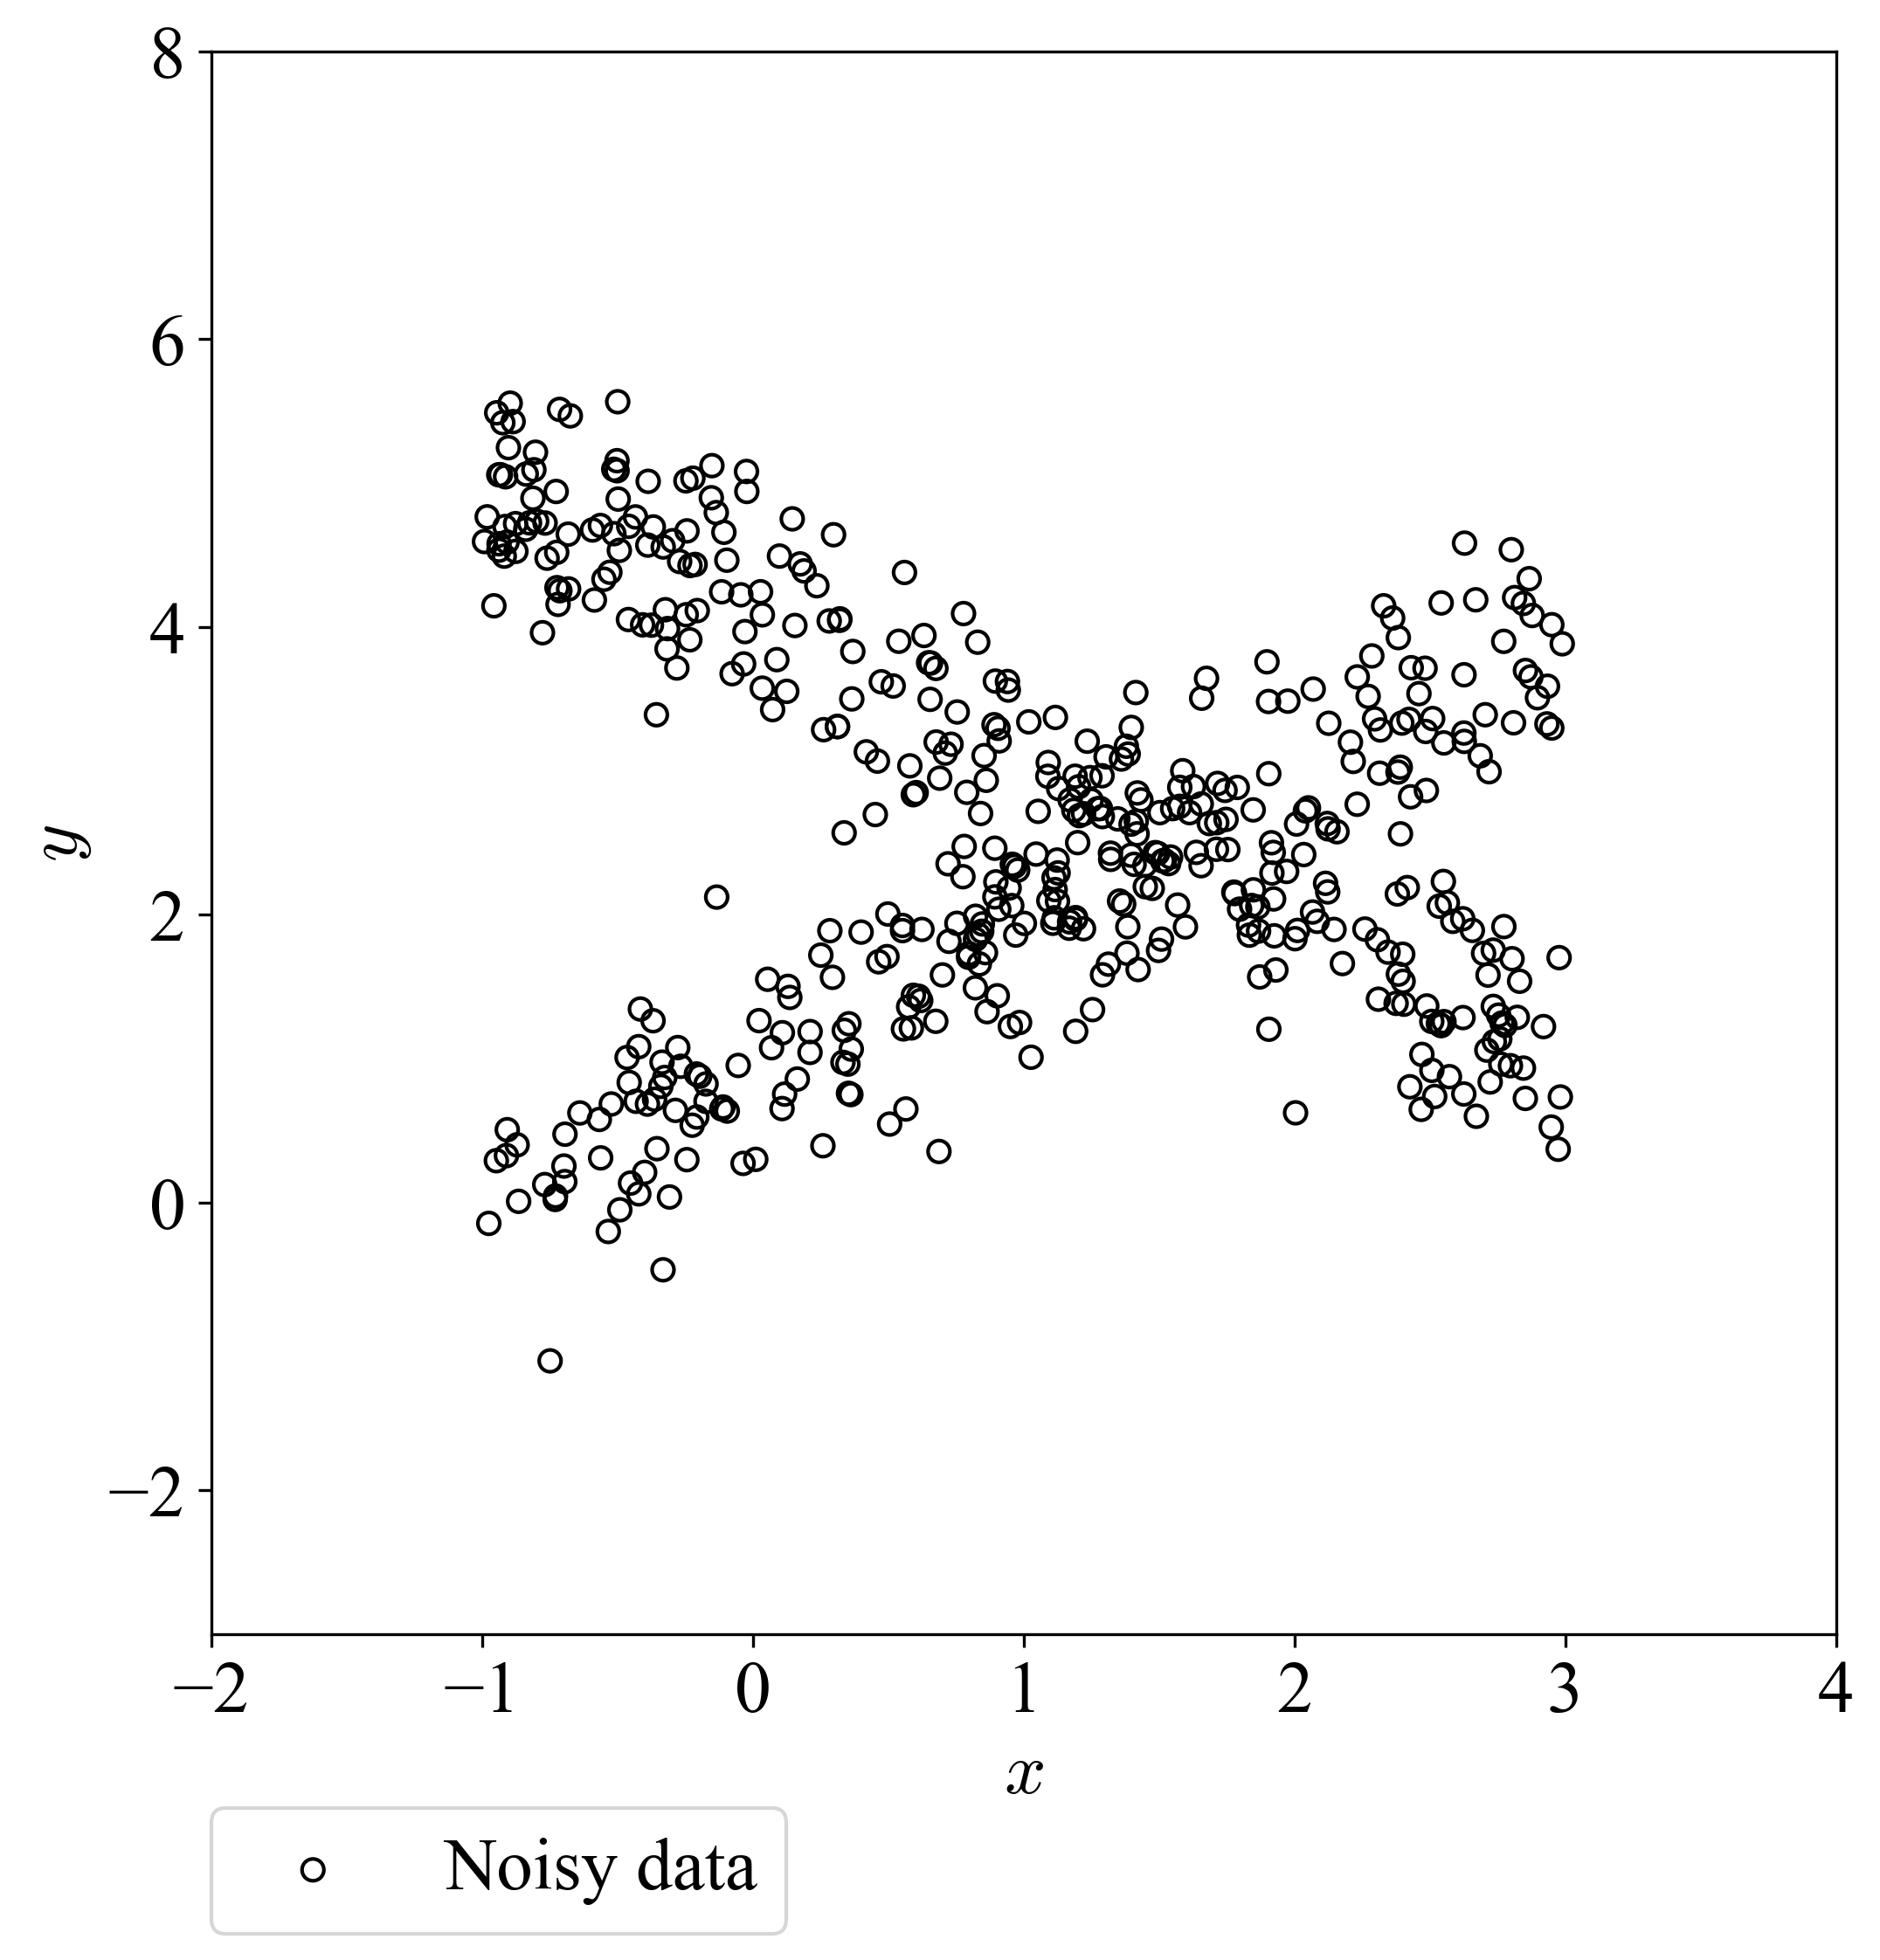
\includegraphics[width = 0.3\textwidth,valign = t]{./newimages/1_1_4_-1_50percent_noisy.png}
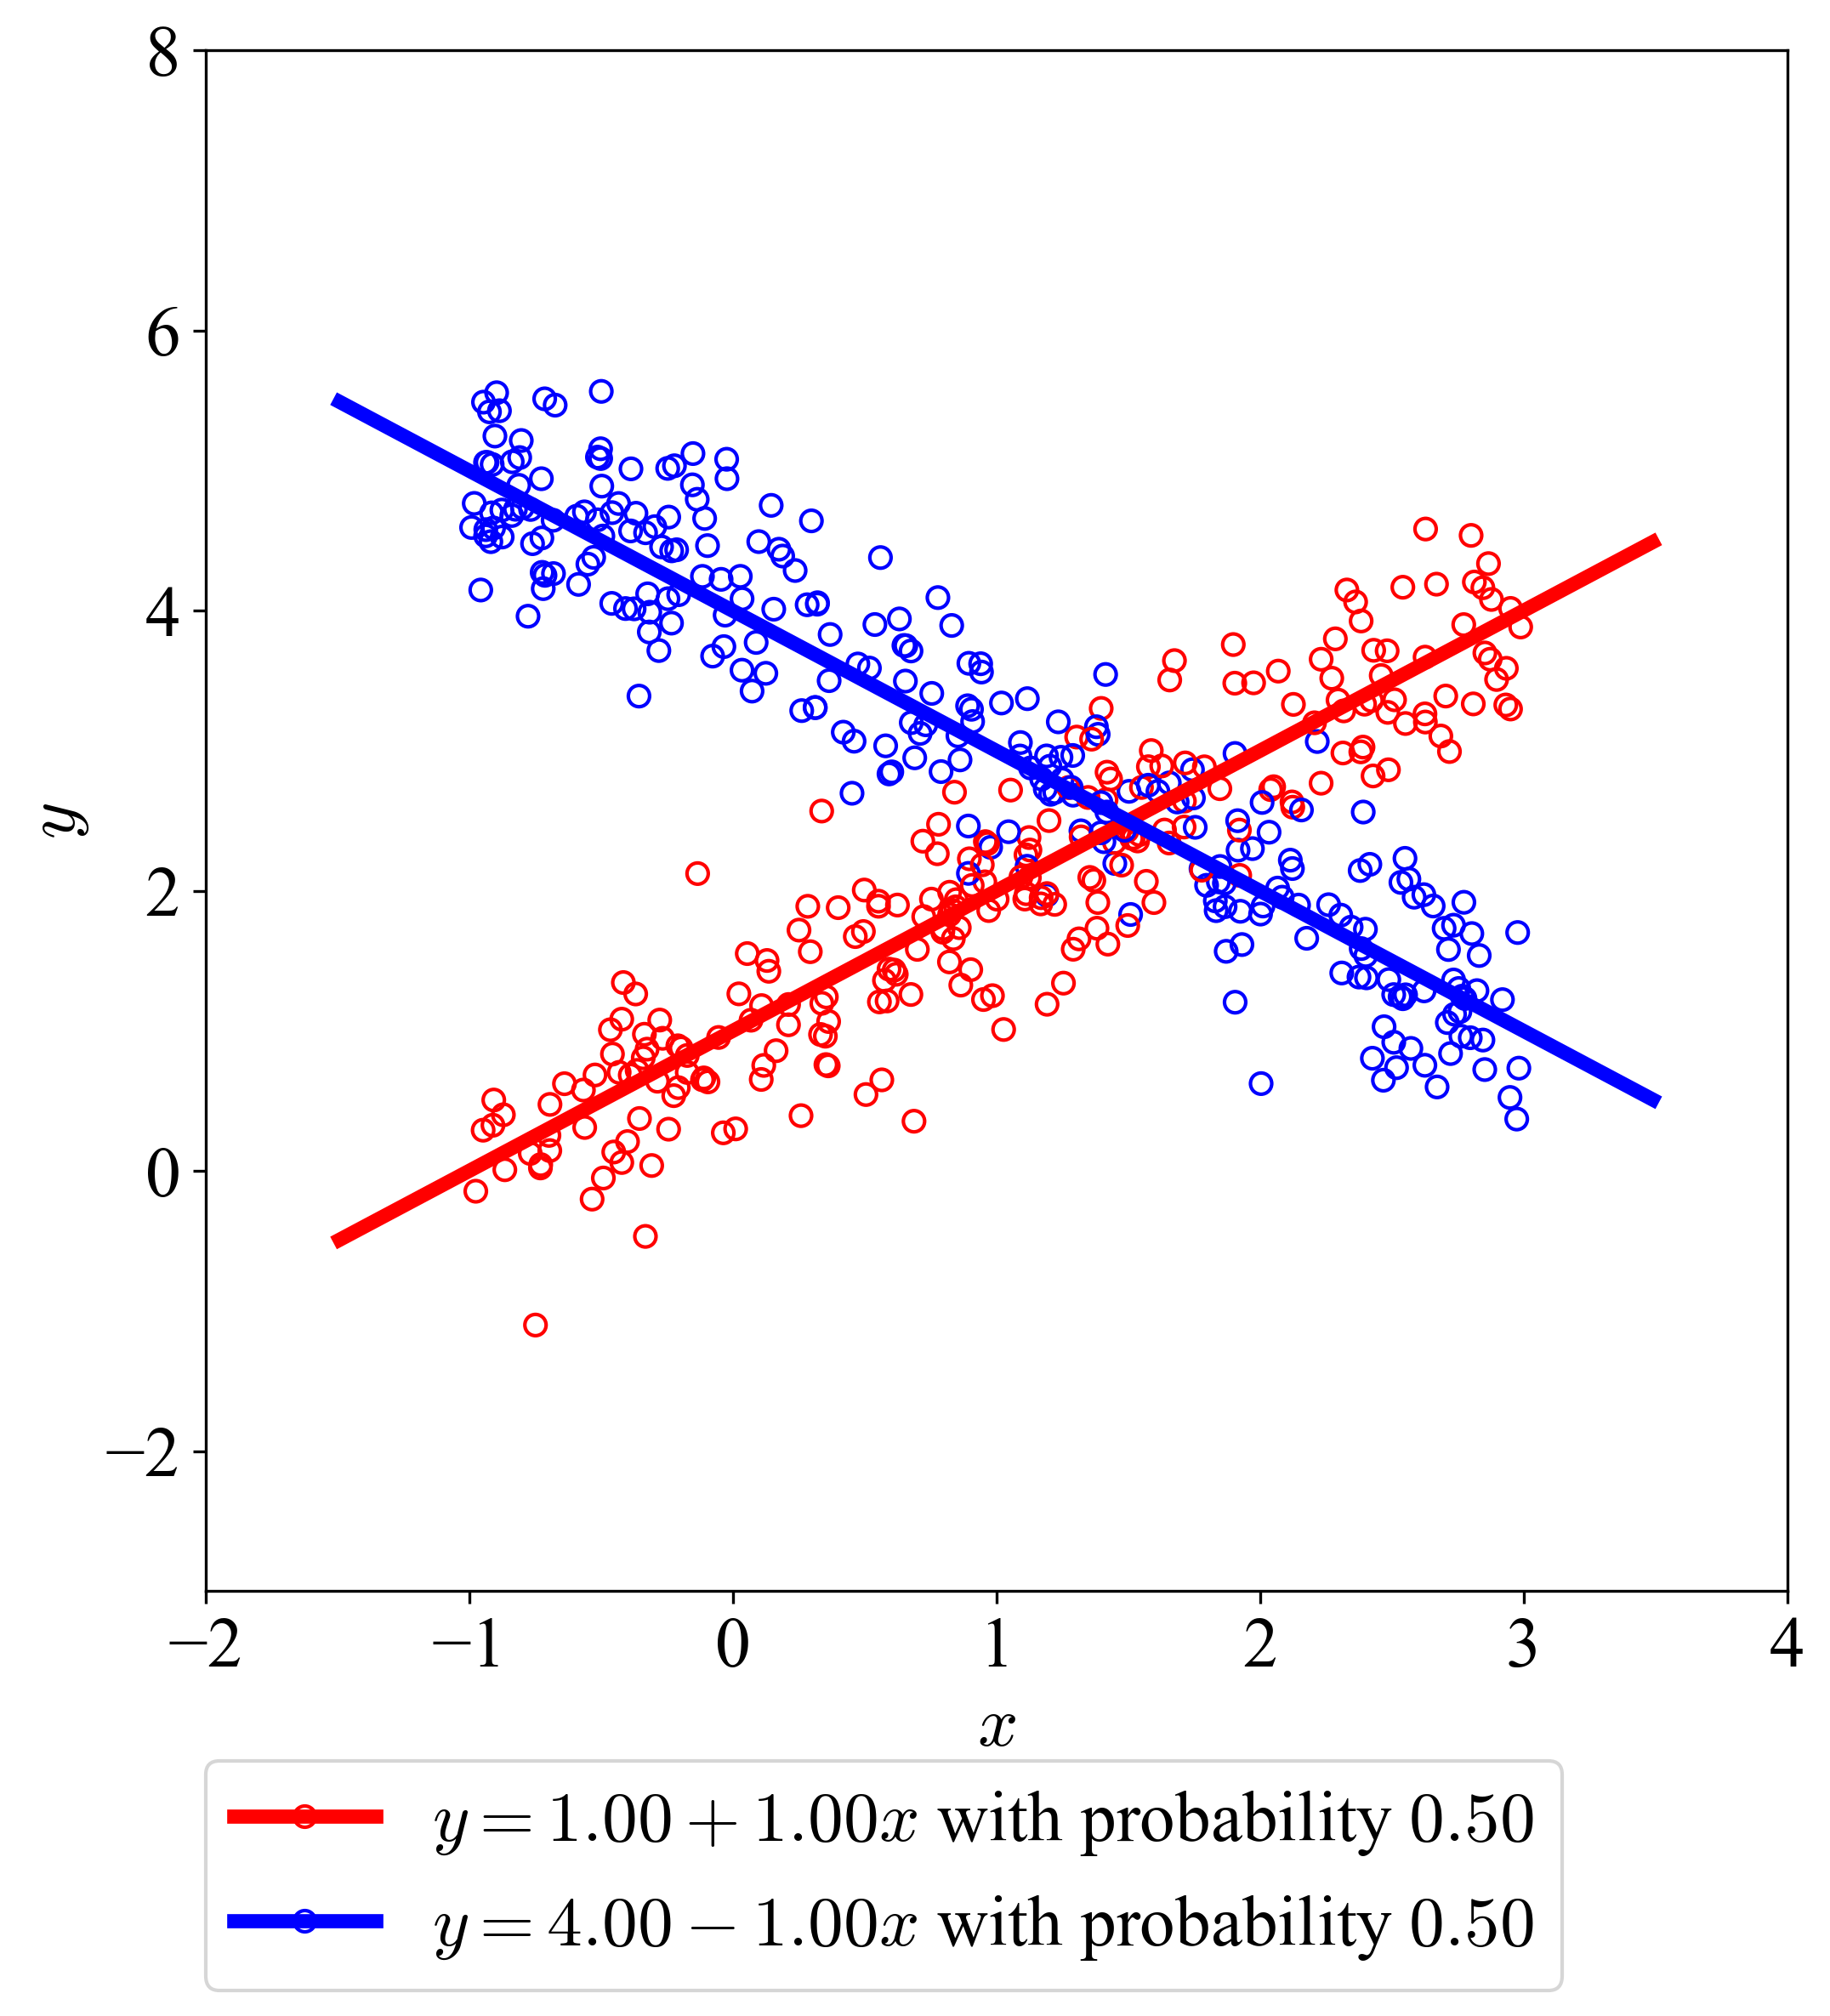
\includegraphics[width = 0.3\textwidth,valign = t]{./newimages/1_1_4_-1_50percent_true.png}
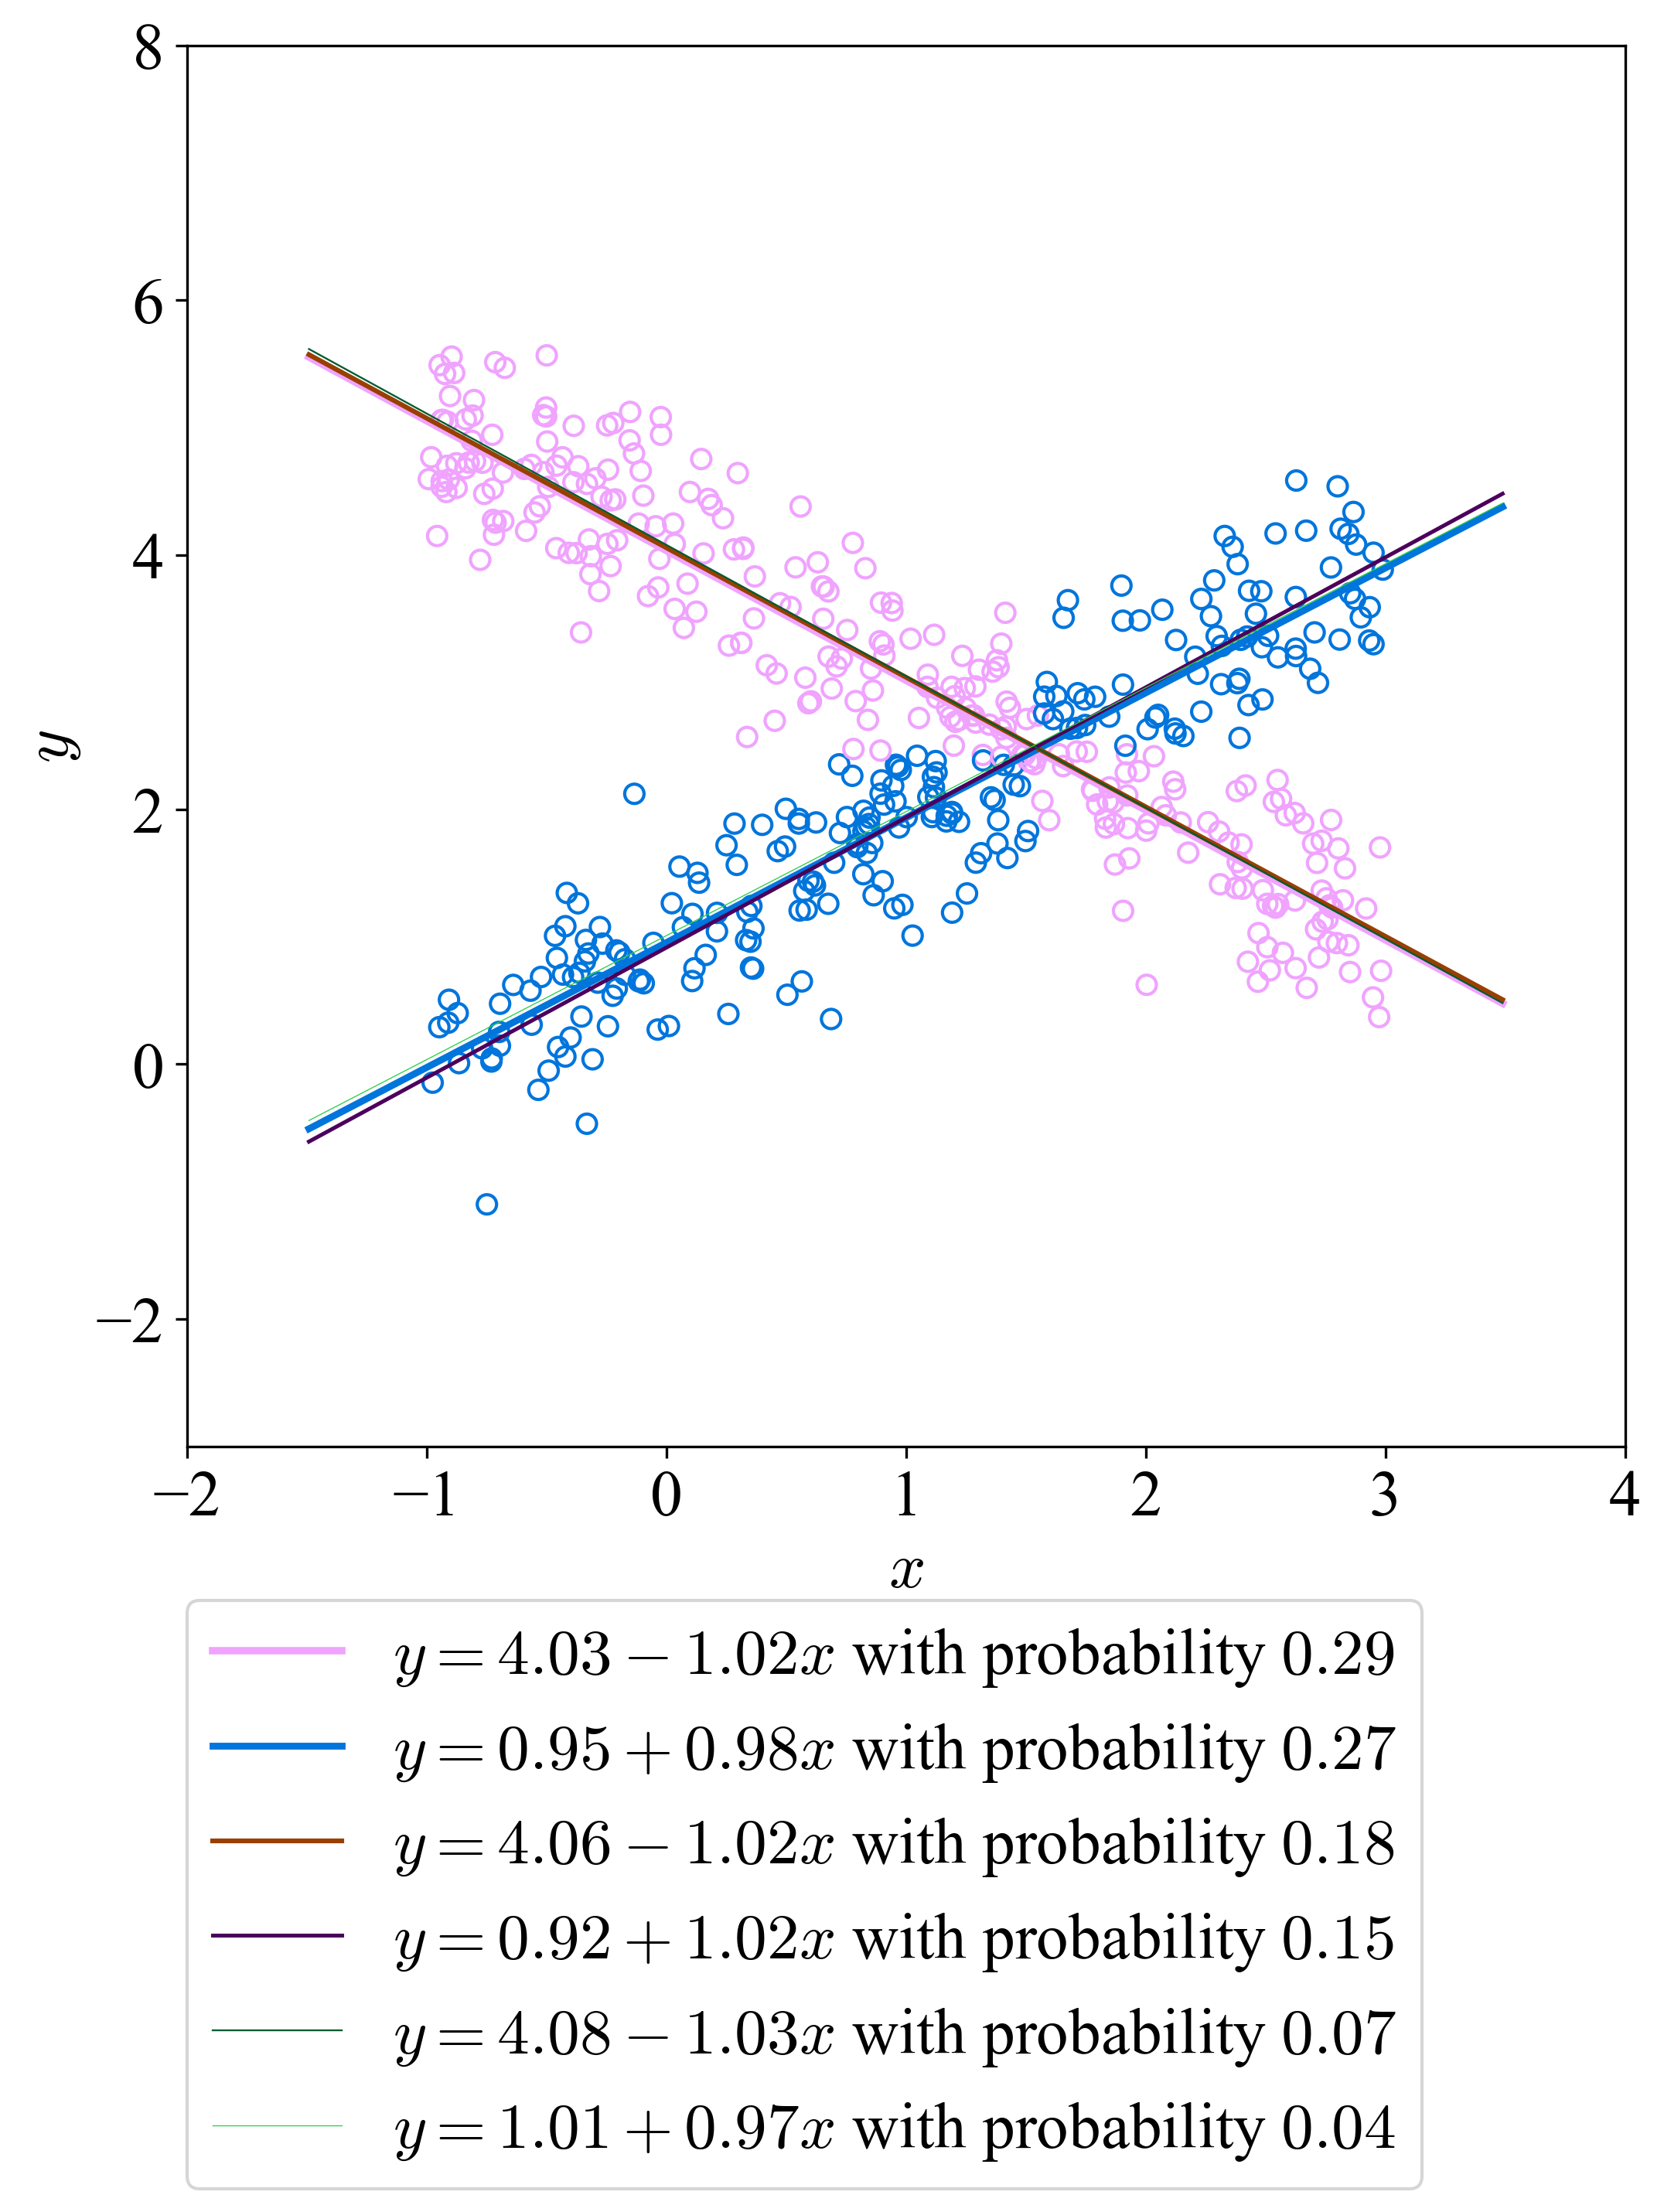
\includegraphics[width = 0.3\textwidth, valign = t]{./newimages/1_1_4_-1_50percent_fitted.png}
\caption{Left: Noisy data; Middle: True mixture; Right: Fitted mixture}
\end{subfigure}
\begin{subfigure}[b]{\textwidth}
\includegraphics[width = 0.9\textwidth]{./newimages/1_1_4_-1_50percent_density.png}
\caption{True and fitted probability density functions (pdf) of $y$ at different $x$'s }
\end{subfigure}
\caption{Two-component concurrent mixture of linear regressions}
\label{fig:2compcorr}
\end{figure}



\noindent{(2)} Two-component parallel mixture: $\sigma = 0.3$. Results are in Figure \ref{fig:2comppara}.

\begin{figure}[!htbp]
\begin{subfigure}[b]{\textwidth}
\includegraphics[width = 0.3\textwidth,valign = t]{./newimages/0_1_1_1_30percent_noisy.png}
\includegraphics[width = 0.3\textwidth,valign = t]{./newimages/0_1_1_1_30percent_true.png}
\includegraphics[width = 0.3\textwidth,valign = t]{./newimages/0_1_1_1_30percent_fitted.png}
\caption{Left: Noisy data; Middle: True mixture; Right: Fitted mixture}
\end{subfigure}

\begin{subfigure}[b]{\textwidth}
\includegraphics[width = 0.9\textwidth]{./newimages/0_1_1_1_30percent_density.png}
\caption{True and fitted probability density functions (pdf) of $y$ at different $x$'s }
\end{subfigure}
\caption{Two-component parallel mixture of linear regressions}
\label{fig:2comppara}
\end{figure}

\noindent{(3)} Three-component mixture: $\sigma = 0.5$. Results are in Figure \ref{fig:3comp}.

\begin{figure}[!htbp]
\begin{subfigure}[b]{\textwidth}
\includegraphics[width = 0.3\textwidth,valign = t]{./newimages/3_-1_1_1dot5_30percent_noisy.png}
\includegraphics[width = 0.3\textwidth,valign = t]{./newimages/3_-1_1_1dot5_30percent_true.png}
\includegraphics[width = 0.3\textwidth,valign = t]{./newimages/3_-1_1_1dot5_30percent_fitted.png}
\caption{Left: Noisy data; Middle: True mixture; Right: Fitted mixture}
\end{subfigure}
\begin{subfigure}[b]{\textwidth}
\includegraphics[width = 0.9\textwidth]{./newimages/3_-1_1_1dot5_30percent_density.png}
\caption{True and fitted probability density functions (pdf) of $y$ at different $x$'s }
\end{subfigure}
\caption{Three-component mixture of linear regressions}
\label{fig:3comp}
\end{figure}


\subsection{Non-discrete mixture} 
\label{section:continuous}

\emph{Data set.} Given the probability measure function $G(\beta)$ and $\sigma$, each data point is generated as follows: (i) $x_i$ is randomly sampled from $\mathrm{Unif}(-3,3)$. (ii) $\beta^i$ is randomly sampled from $G(\beta)$. (iii) $y_i = \beta^i_1 +\beta^i_2 x_i +\epsilon_i$, where $\epsilon_{ij} \sim N(0,\sigma^2)$ is noise and $\sigma = 0.5$. We set $G(\beta)$ as a mixture of two Gaussians, 
\[
\begin{split}
\gamma_1 \sim & N\left( \begin{pmatrix} 1\\ 0.5\end{pmatrix}, \begin{pmatrix} 0.5 & 0.2\\ 0.2& 0.3\end{pmatrix} \right)\\
\gamma_2 \sim & N\left( \begin{pmatrix} 2\\ 3\end{pmatrix}, \begin{pmatrix} 0.5 & 0.2\\ 0.2& 0.3\end{pmatrix} \right)\\
\beta = &(1-\Delta)\cdot \gamma_1 + \Delta\cdot \gamma_2
\end{split}
\]
where $\Delta \in \{ 0, 1\}$ with $\PP(\Delta = 1) = 0.5$. 

\emph{Implementation. } In this case, we recommend using randomized initialization when solving the non-convex subproblem for better convergence performance. More specifically, at iteration $t$ of CGM, the subproblem on line 3 of Algorithm \ref{CGM} is solved with initialization at $\gv^{\beta_t}$ with $\beta_t$ randomly sampled from $\mathrm{Unif}[-10,10]$. We choose $x$ from $(-4,4)$ as well as one value $5.0$ outside the interval $(-4,4)$  to evalute their generalization accuracy. Our implementation of the expectation-maximization algorithm follows the standard form in \citet{faria2010fitting}. To be fair in the comparsion, we feed the expectation-maximization algorithm with the true $\sigma$ value, and $\beta$ is also initialized randomly by sampling uniformly from $[-10,10]^2$ in the \EM algorithm.

\emph{Plots. } The results are shown in Figure \ref{fig:continuous}. It is remarkable that $G$ is actually not compact here, but the algorithm achieves excellent accuracy. Specifically, in Figure \ref{fig:continuous}(b), the fitted density function is much more close to the ground truth compared to the two-component mixture fitted by the \EM algorithm.

\begin{figure}[!htbp]
\begin{subfigure}[b]{\textwidth}
\includegraphics[width = 0.3\textwidth,valign = t]{./newimages/continuous50050percentCGM_noisy.png}
\includegraphics[width = 0.3\textwidth,valign = t]{./newimages/continuous50050percentEM10_fitted.png}
\includegraphics[width = 0.3\textwidth,valign = t]{./newimages/continuous50050percentCGM_fitted.png}
\caption{Left: Noisy data; Middle: Fitted mixture by two-component EM; Right: Fitted mixture by CGM}
\end{subfigure}

\begin{subfigure}[b]{\textwidth}
\includegraphics[width = 0.9\textwidth]{./newimages/continuous50050percentEM10_density.png}
\includegraphics[width = 0.9\textwidth]{./newimages/continuous50050percentCGM_density.png}
\caption{True and fitted probability density functions (pdf) of $y$ at different $x$'s: Two-component EM (top) and CGM (bottom) }
\end{subfigure}
\caption{Non-discrete mixture }
\label{fig:continuous}
\end{figure}



\subsection{Nonlinear regression}
\label{section:nonlinear}
\emph{Data set.} (a) Polynomial regressions: Given the probability measure function $G(\beta)$ and $\sigma$, each data point is generated as follows: (i) $x_i$ is randomly sampled from $\mathrm{Unif}(-1,1.5)$. (ii) $\beta^i$ is randomly sampled from $G(\beta)$. (iii) $y_i = \beta^i_1(\beta^i_1+\beta^i_2) +0.5 \beta^i_1\beta^i_2 x_i +0.5\beta^i_1x_i^2+\epsilon_i$, where $\epsilon_{ij} \sim N(0,\sigma^2)$ is noise and $\sigma =0.5$. We set $G$ as a two-component mixture here with $\beta = (0.5,2)$ with probability $0.5$ and $\beta = (1,2.5)$ with probability $0.5$. (b) Exponential regression: Given the probability measure function $G(\beta)$ and $\sigma$, each data point is generated as follows: (i) $x_i$ is randomly sampled from $\mathrm{Unif}(-1,3)$. (ii) $\beta^i$ is randomly sampled from $G(\beta)$. (iii) $y_i = \beta^i_1 + \exp(-\beta^i_2 x)$, where $\epsilon_{ij} \sim N(0,\sigma^2)$ is noise and $\sigma =0.5$. We set $G$ as a two-component mixture here with $\beta = (-0.5,1)$ with probability $0.5$ and $\beta = (-1.5,1.5)$ with probability $0.5$.


\emph{Implementation. } We use randomized initialization when solving the non-convex subproblem for better convergence performance. More specifically, at iteration $t$ of CGM, the subproblem on line 3 is solved with initialization at $\gv^{\beta_t}$ with $\beta_t$ randomly sampled from $\mathrm{Unif}[-10,10]$. 

\emph{Plots. } The results are shown in Figure \ref{fig:continuous} and \ref{fig:exponential}.

\begin{figure}[!htbp]
\begin{subfigure}[b]{\textwidth}
\includegraphics[width = 0.3\textwidth,valign = t]{./newimages/polynomial_noisy.png}
\includegraphics[width = 0.3\textwidth,valign = t]{./newimages/polynomial_true.png}
\includegraphics[width = 0.3\textwidth,valign = t]{./newimages/polynomial_fitted.png}
\caption{Left: Noisy data; Middle: True mixture; Right: Fitted mixture}
\end{subfigure}

\begin{subfigure}[b]{\textwidth}
\includegraphics[width = 0.9\textwidth]{./newimages/polynomial_density.png}
\caption{True and fitted probability density functions at different $x$'s }
\end{subfigure}
\caption{Mixture of polynomial regressions}
\label{fig:polynomial}
\end{figure}

\begin{figure}[!htbp]
\begin{subfigure}[b]{\textwidth}
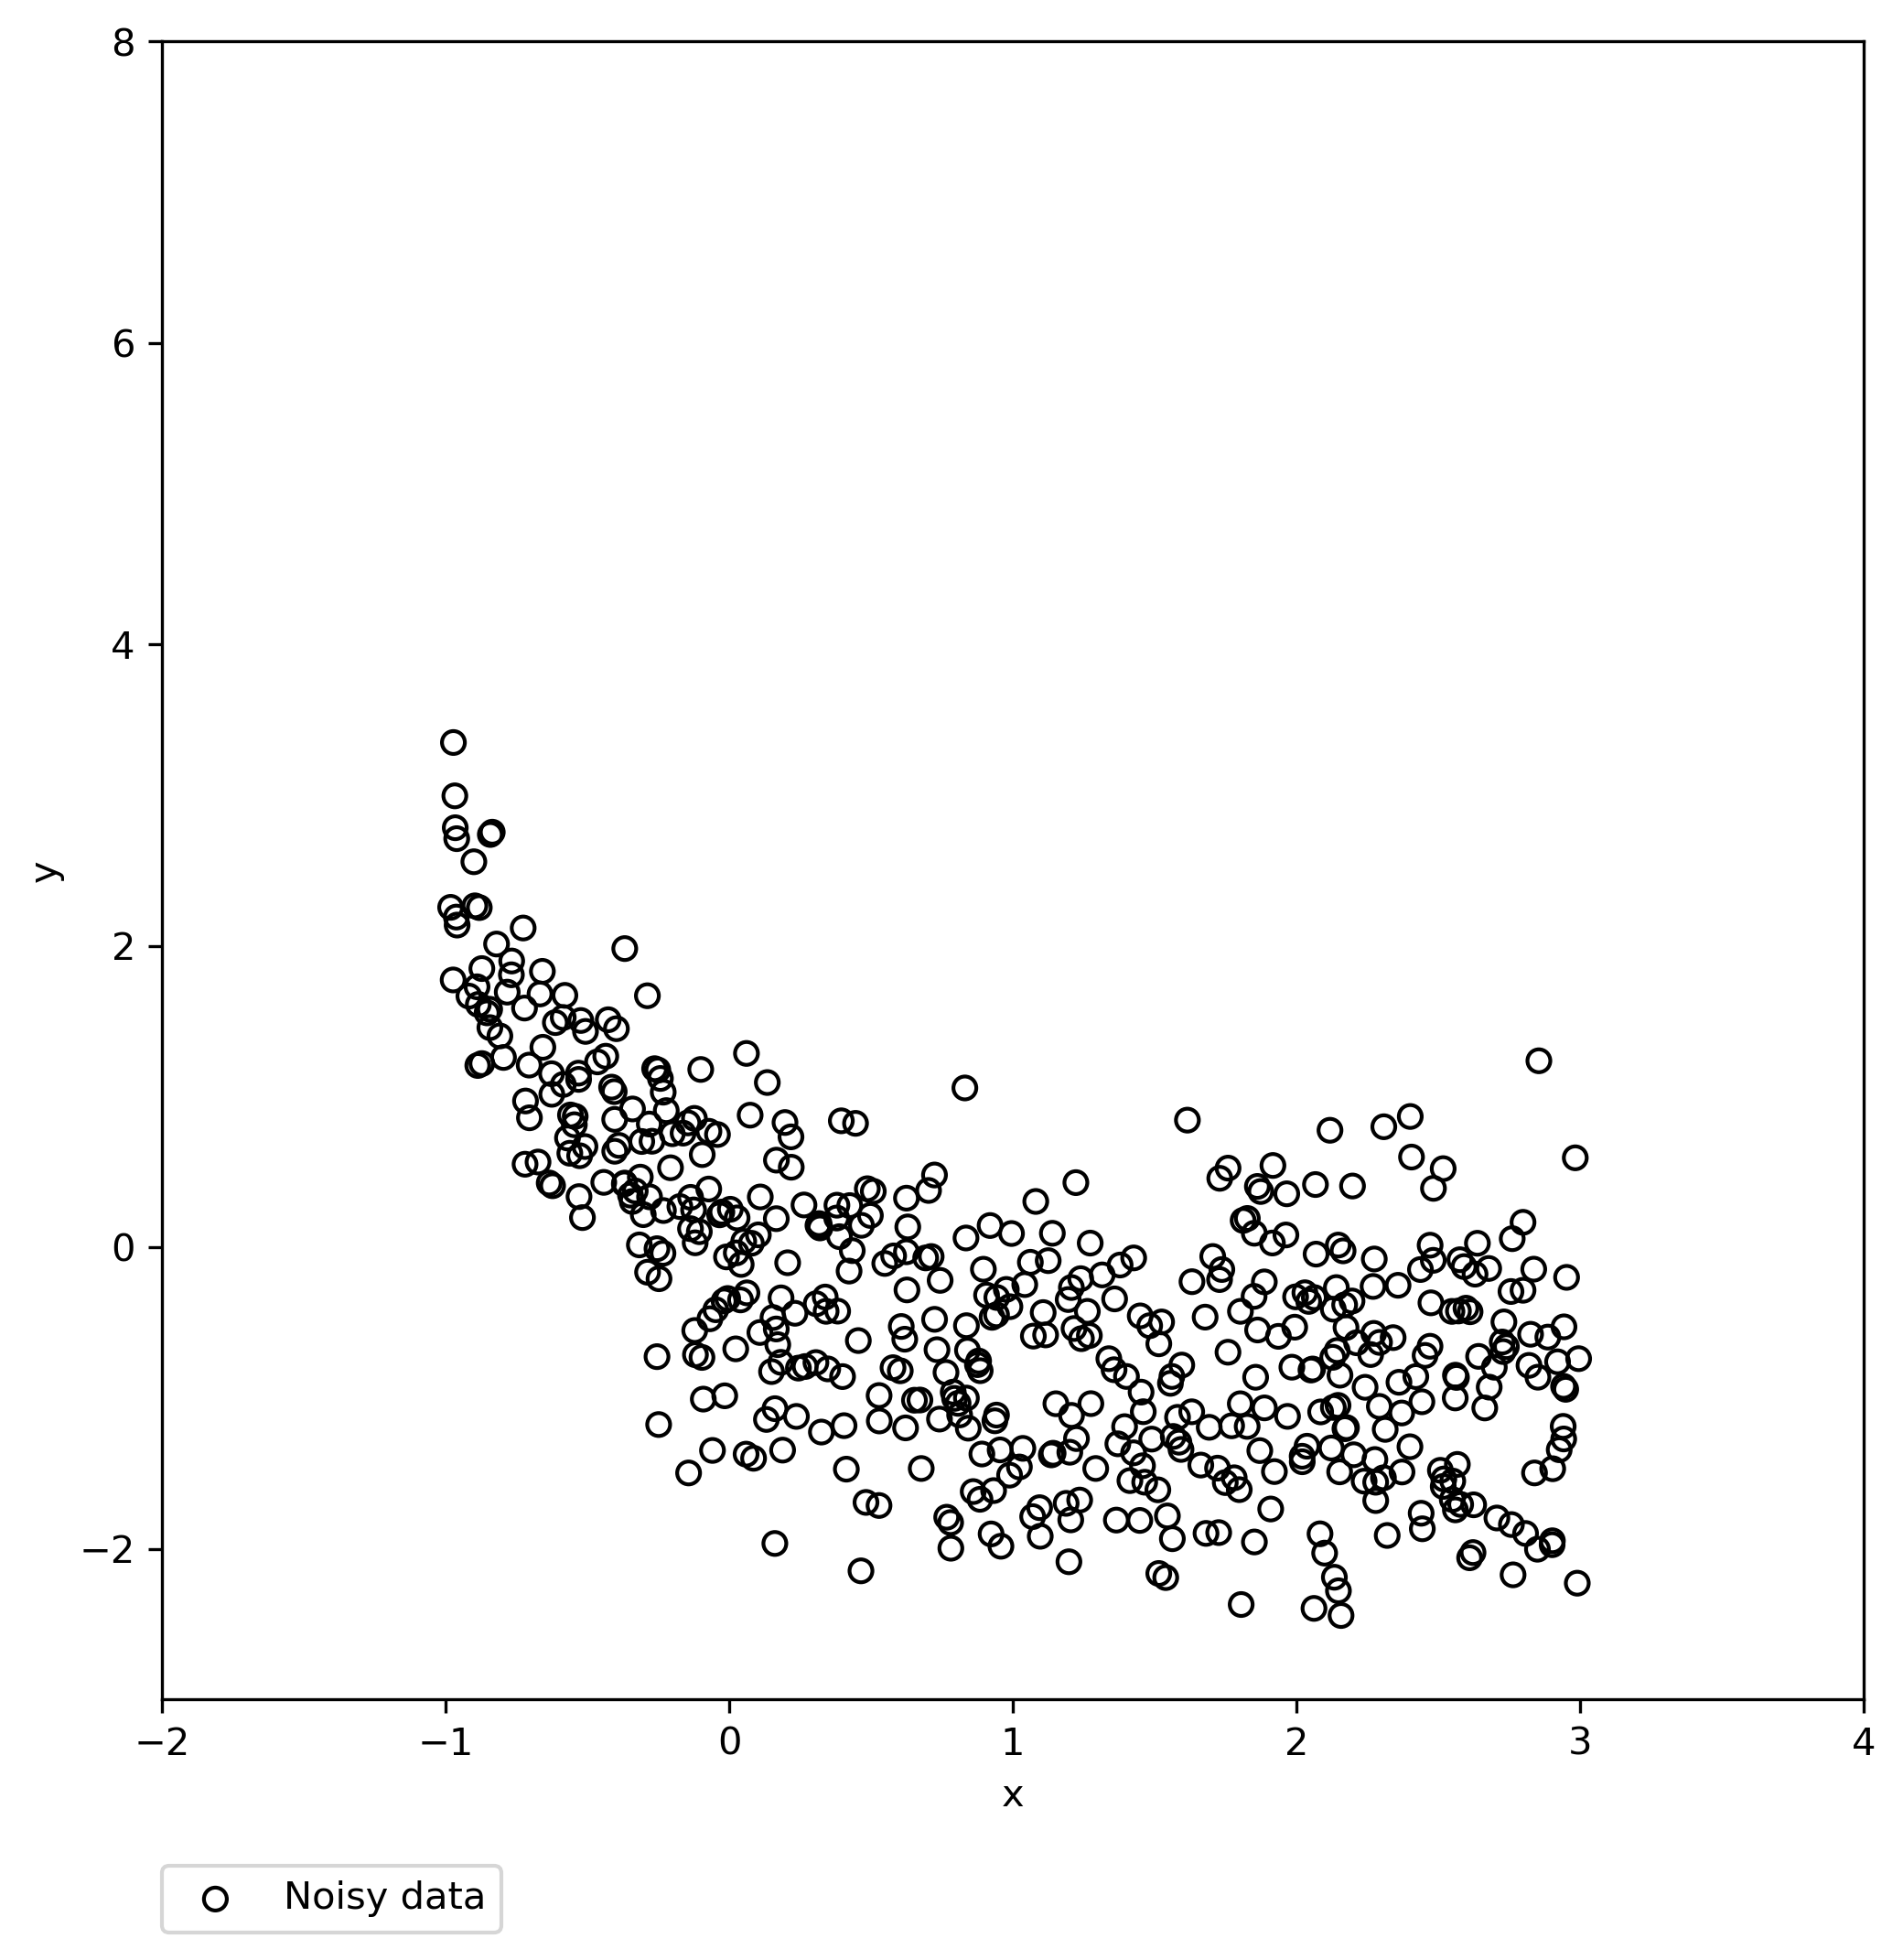
\includegraphics[width = 0.3\textwidth,valign = t]{./newimages/exponential_noisy.png}
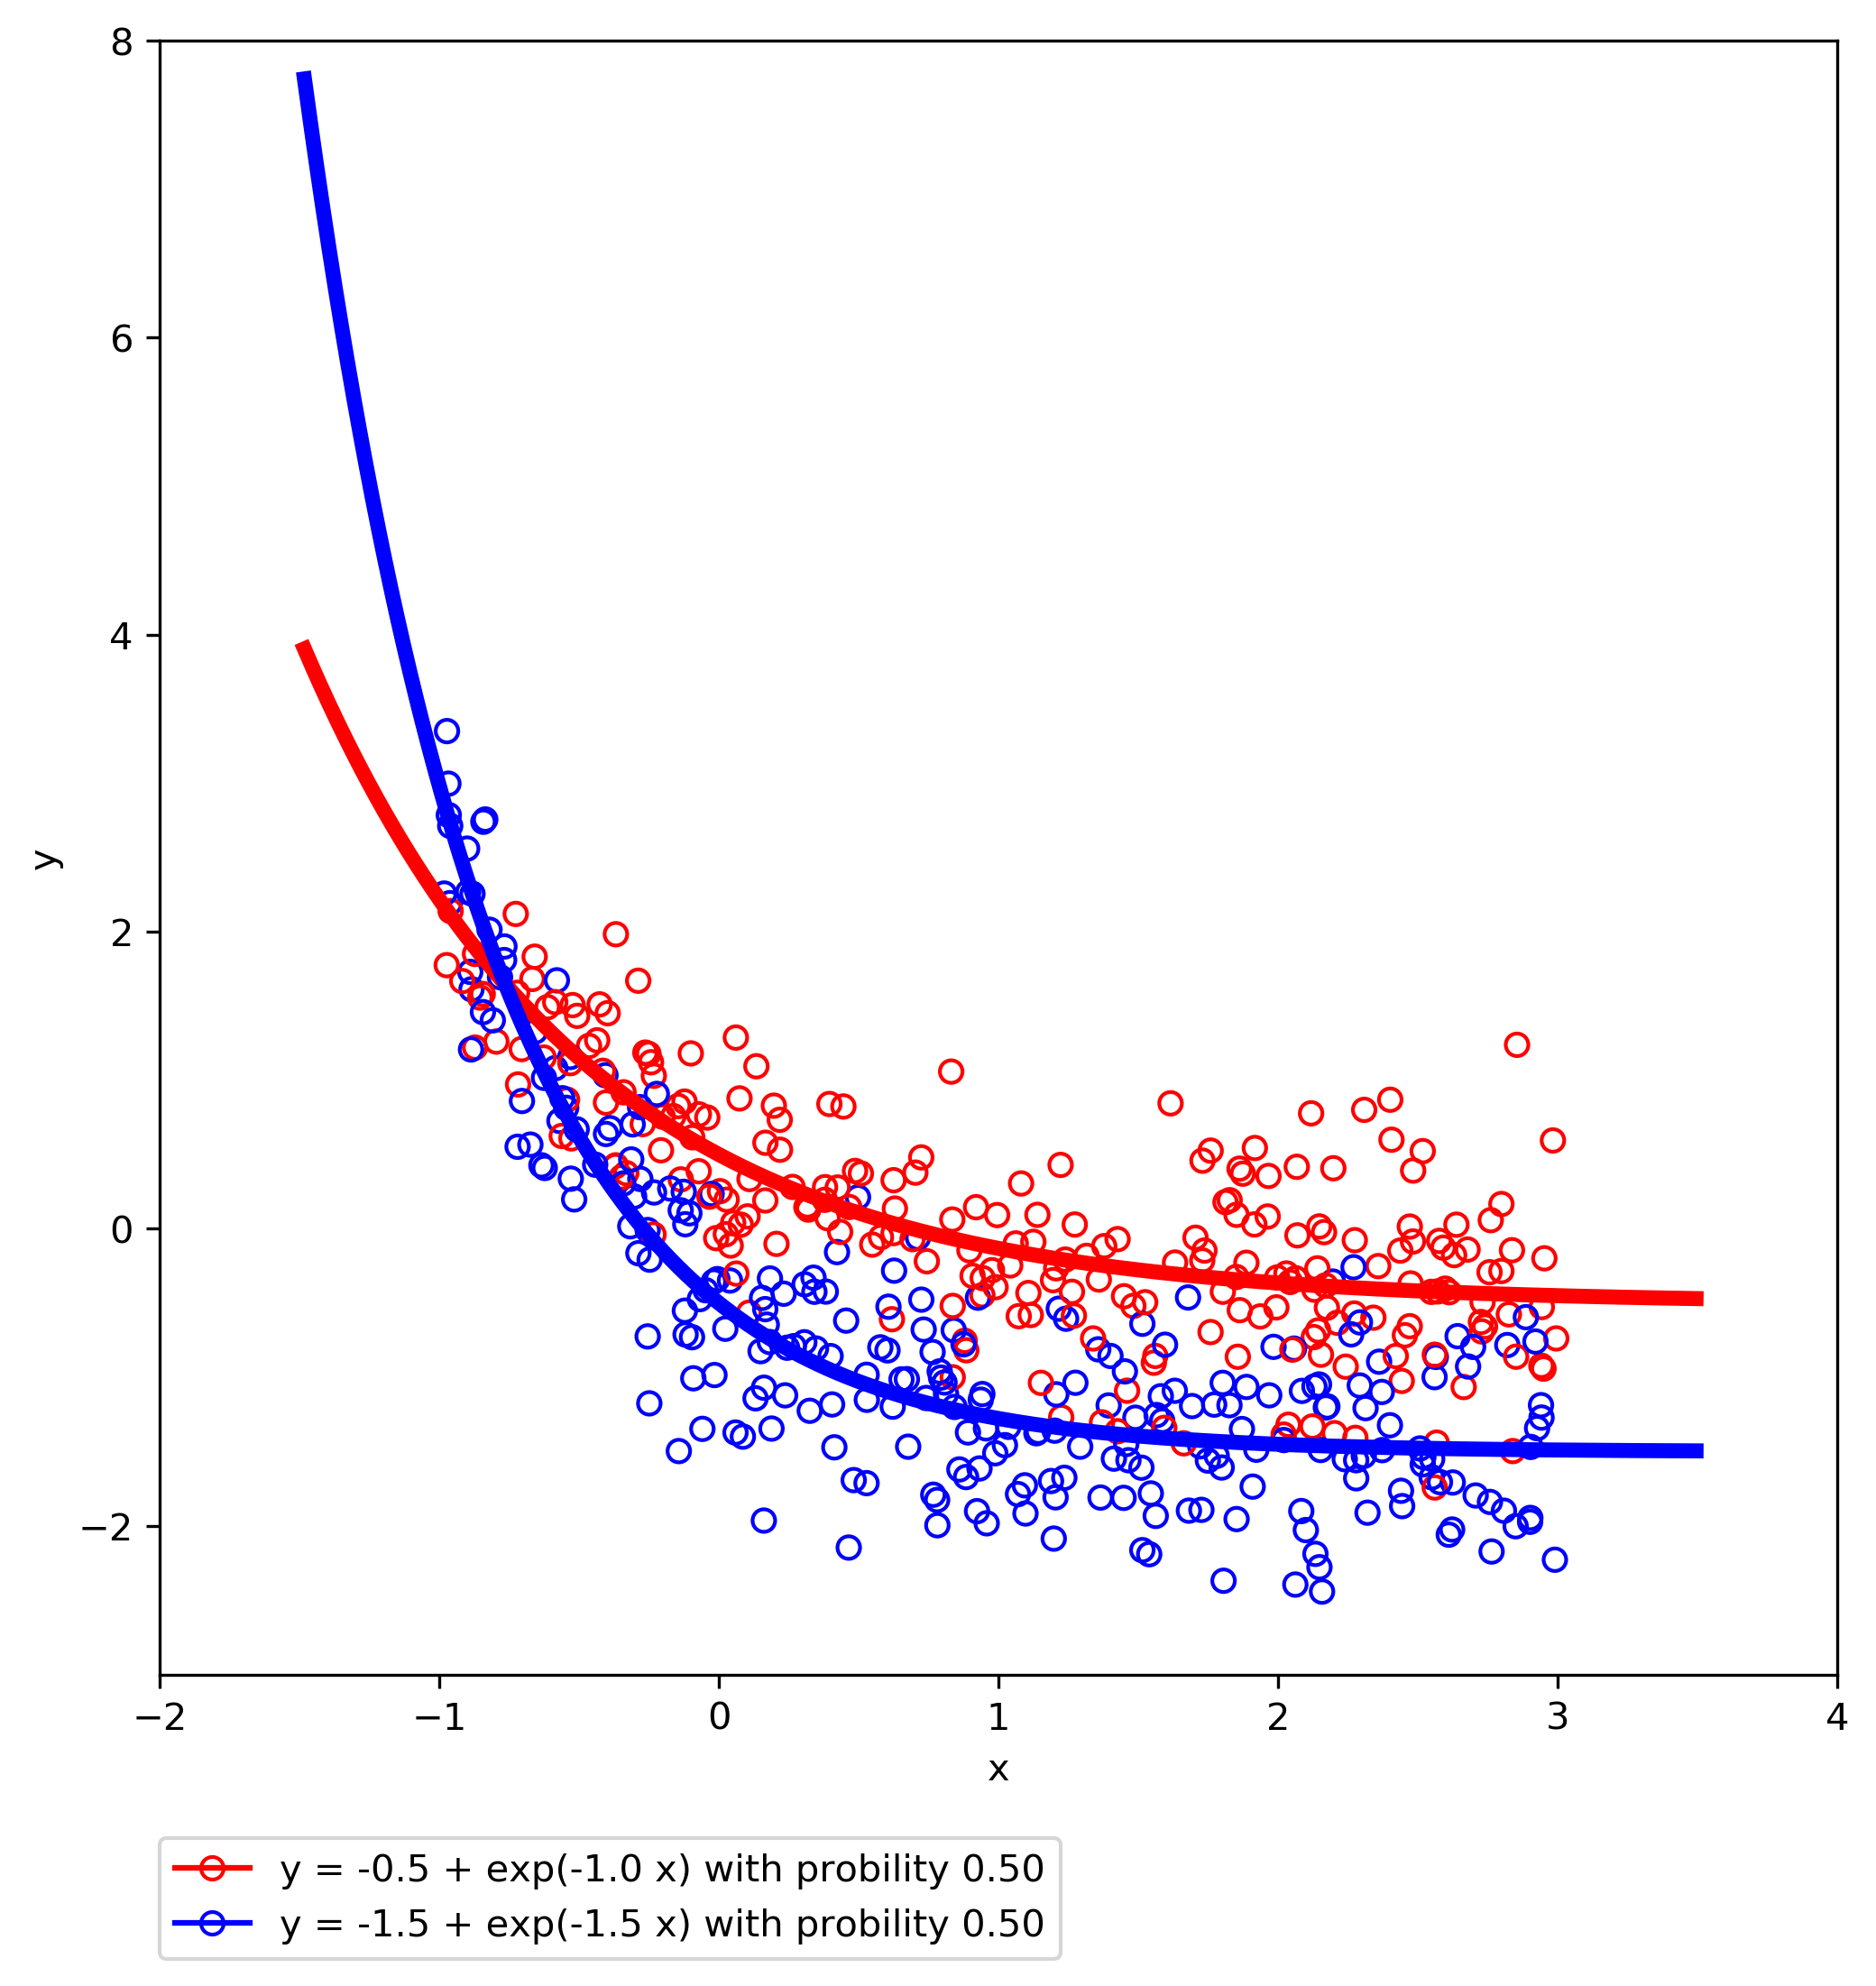
\includegraphics[width = 0.3\textwidth,valign = t]{./newimages/exponential_true.png}
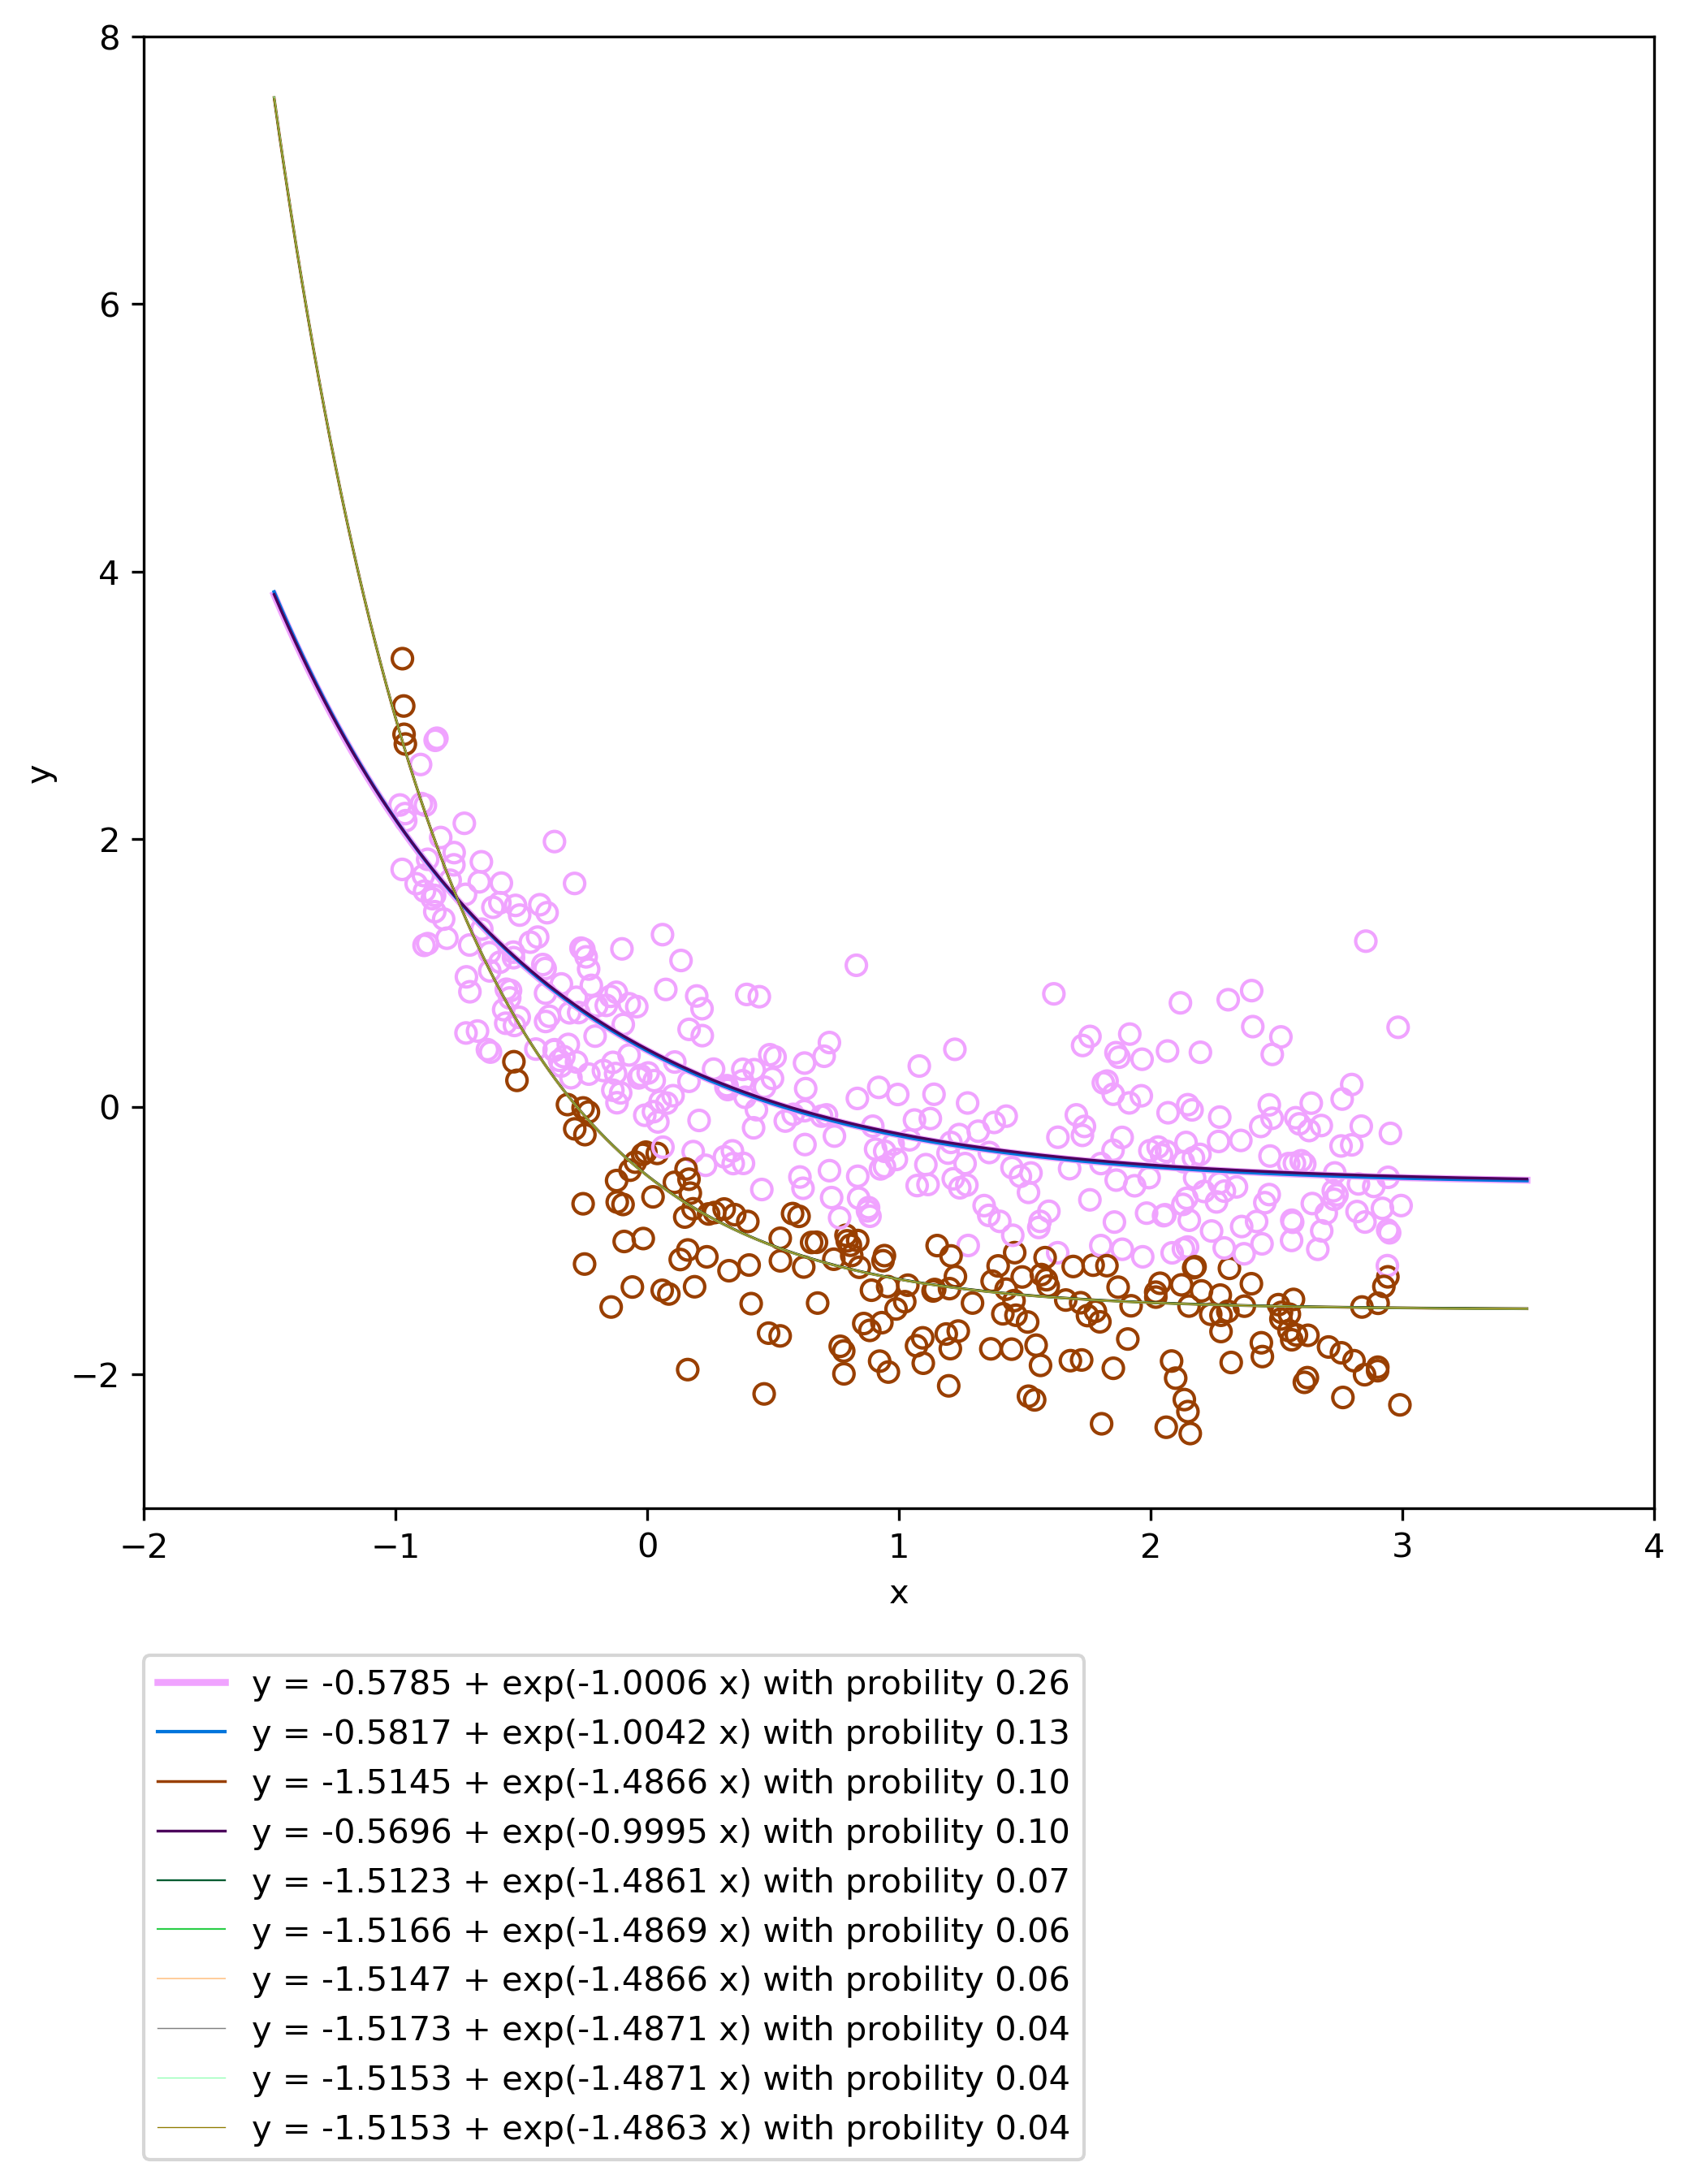
\includegraphics[width = 0.3\textwidth,valign = t]{./newimages/exponential_fitted.png}
\caption{Left: Noisy data; Middle: True mixture; Right: Fitted mixture.}
\end{subfigure}

\begin{subfigure}[b]{\textwidth}
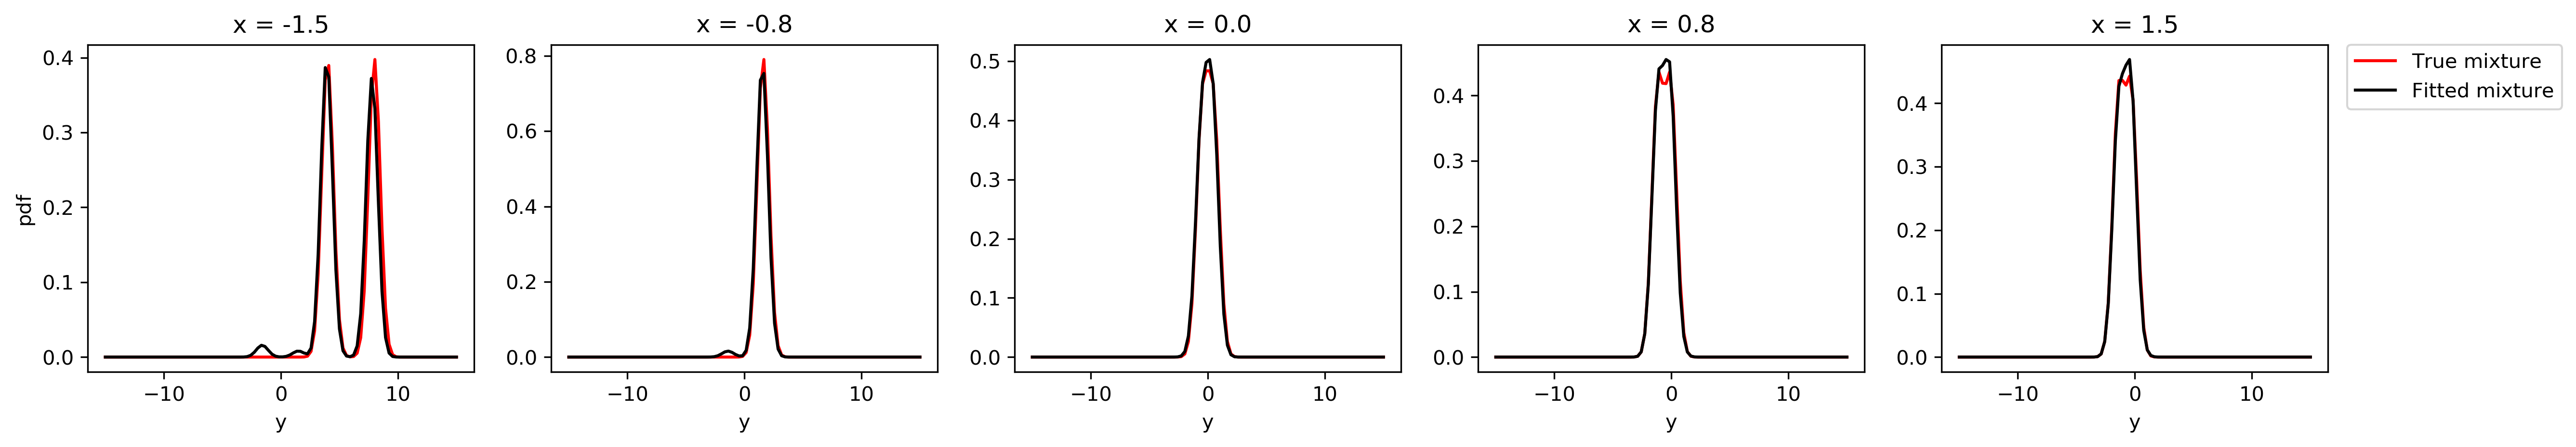
\includegraphics[width = 0.9\textwidth]{./newimages/exponential_density.png}
\caption{True and fitted probability density functions at different $x$'s }
\end{subfigure}
\caption{Mixture of exponential regressions}
\label{fig:exponential}
\end{figure}

In our numerical experiments, the number of simulations $T$ (10 to 100) is usually much smaller than the number of data points $n$ (300 to 500), so the number of support points never exceed the theoretical characterization upper bound $n$. However, an index limitation step \citep[Section 4.2]{mallet1986maximum} can be enforced to replace any iteration with more than $n$ support points by a new iteration with at most $n$ support points.




\section{Numerical experiments on real data}
\label{section:realdata}

\subsection{Tone perception data}

The tone perception data originally comes from experiments by \citet{cohen1980inharmonic} and has been analyzed in the statistics literature by \citet{de1989mixtures}, \citet{viele2002modeling} and \citet{yao2015mixtures}. A trained musician is presented with a pure fundamental tone plus a series of stretched overtones, and the experiment is repeated a few times with different tones. The regressor value $x$ is the stretching ratio of the overtone to the fundamental tone. The musician is then asked to tune an adjustable tone to the octave above the fundamental tone. The response value $y$ is the ratio of the adjusted tone to the fundamental. The experiment is designed to verify if either of the two existing theories of music perception is valid: one theory states that the adjusted tone is at ratio $2:1$ to the fundamental tone, while the other theory states that the adjusted tone will be equal to the overtone. In the language of linear regression, two existing theories correspond to $y = 2$ and $y = x$ respectively. The data is available in R package \texttt{mixtools} \citep{R} containing $150$ data points from one musician. The result of fitting data with mixture of linear regressionss is shown in Figure \ref{fig:tonedata}. The noise level $\sigma$ is chosen as $0.2$.


\subsection{Aphids data}
The aphids data was firstly analyzed in \citet{boiteau1998rate}. The data comes from the study on spreading of tobacco plants virus by aphids. The regressor value $x$ is the number of aphids that were released in a closed chamber containing 12 infected and 69 healthy tobacco plants. The response value $y$ is the number of infected plants amongst those previously healthy after 24 hours. The data is currently available in R package \texttt{mixreg} \citep{boiteau1998rate} containing 51 independent experiments. The result of fitting data with mixture of linear regressionss is shown in Figure \ref{fig:aphidsdata}. The noise level $\sigma$ is chosen as $0.2$.

\begin{figure}[!htbp]
\begin{subfigure}{0.5\textwidth}
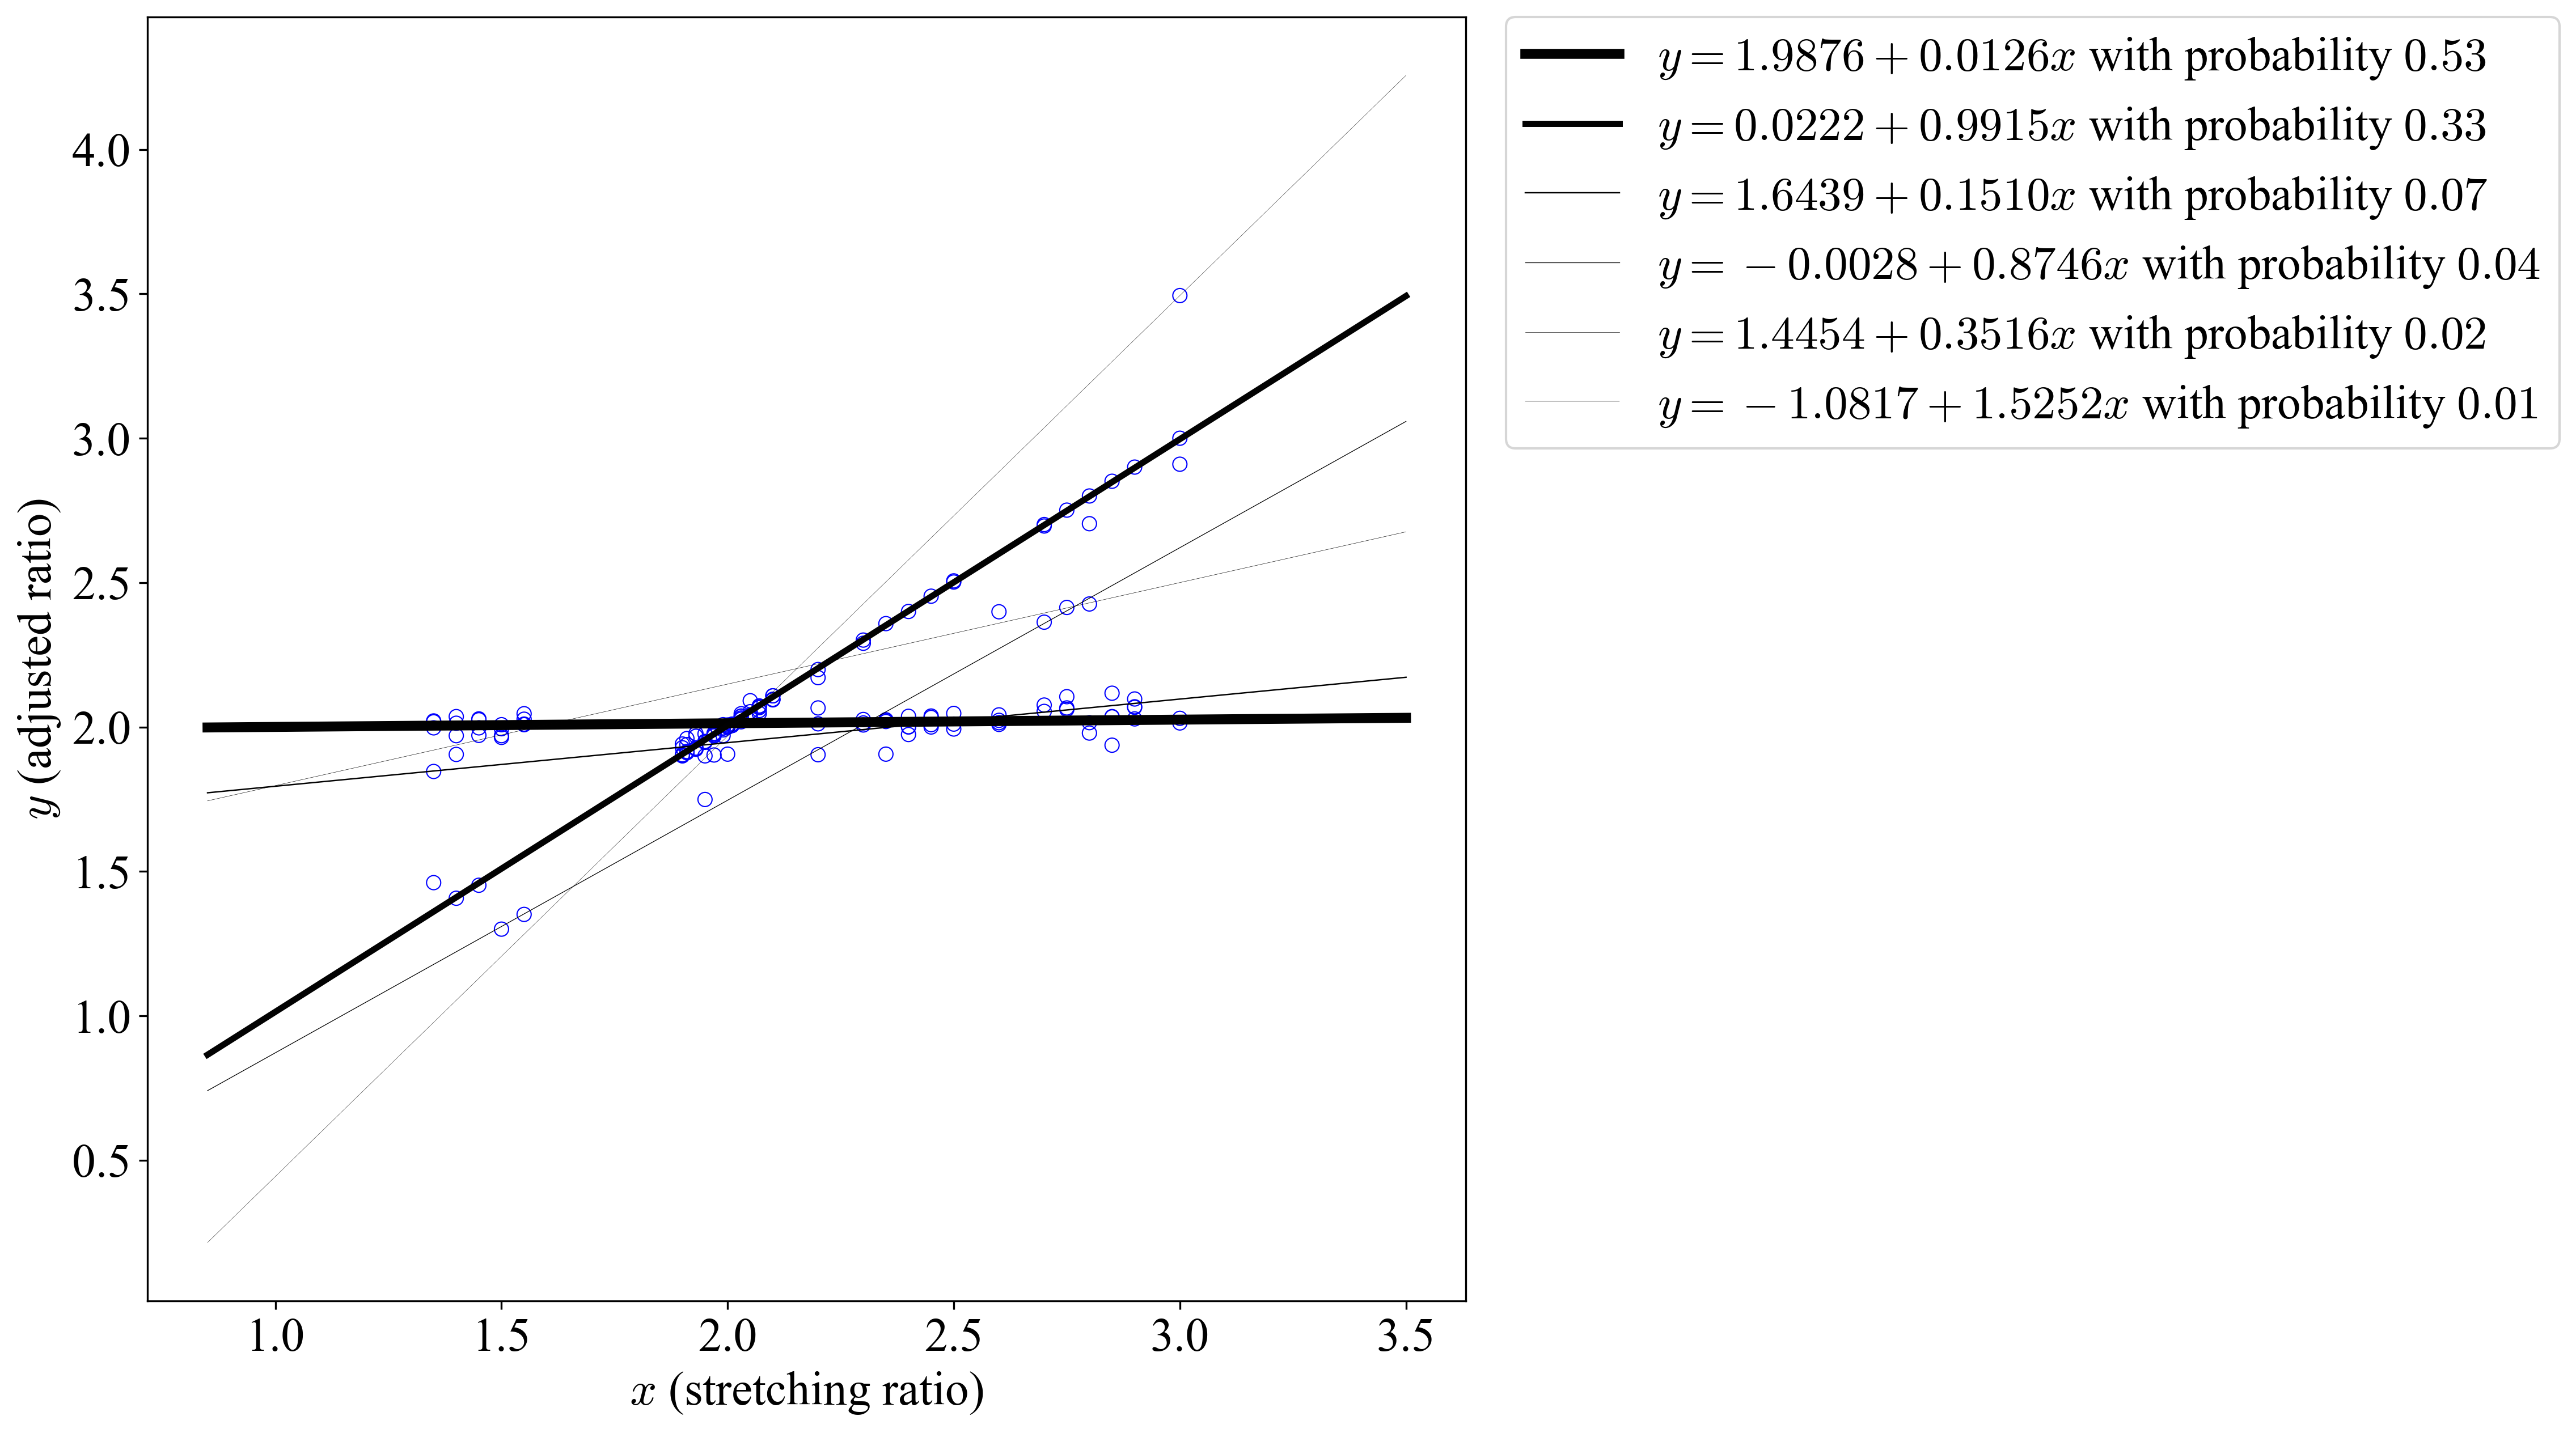
\includegraphics[width = \textwidth]{./newimages/tone.png}
\caption{Fitting music tone perception data}
\label{fig:tonedata}
\end{subfigure}
\begin{subfigure}{0.5\textwidth}
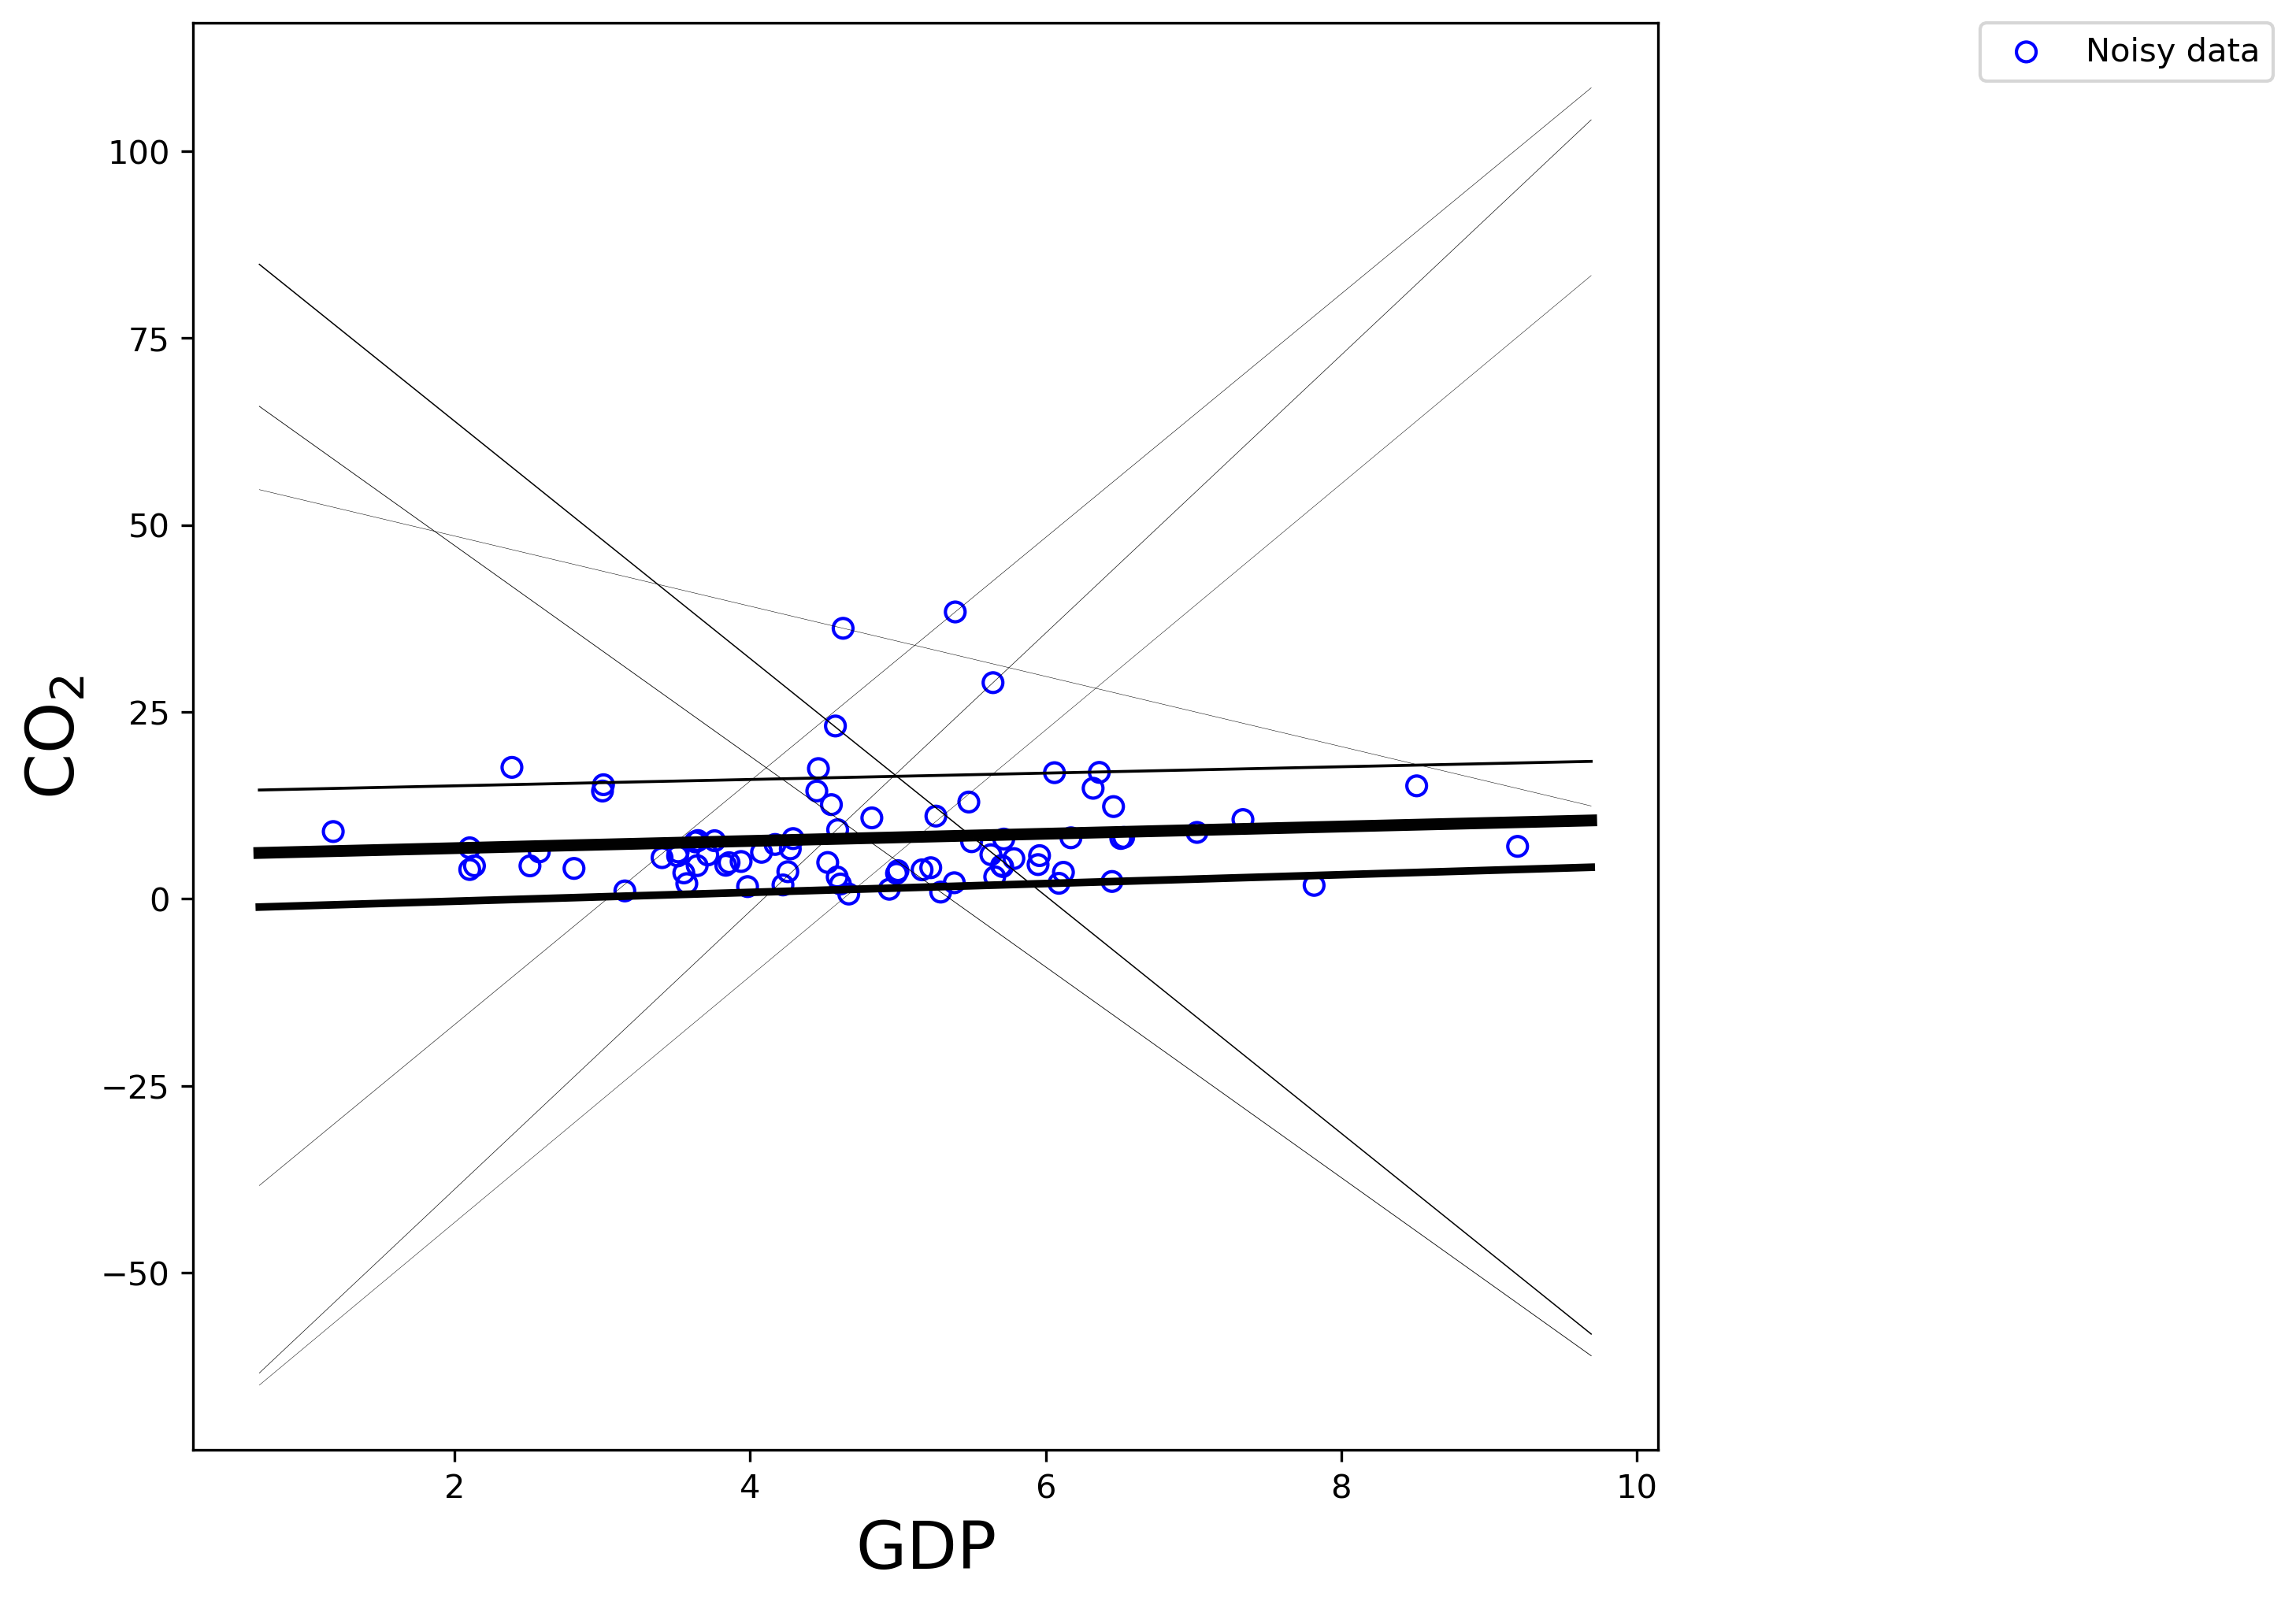
\includegraphics[width = \textwidth]{./newimages/aphids.png}
\caption{Fitting aphids data}
\label{fig:aphidsdata}
\end{subfigure}
\caption{Real data experiments}
\end{figure}

\section{Conclusions}

\label{section:conclusions}
We propose to fit mixture of linear regressions  with the nonparametric maximum likelihood estimators. Concretely, we provide both algorithmic advances and detailed theoretical analysis. It is of interest to establish the error bound for other sorts of mixture of regressions model as well, such as multivariate linear regressions and logistic regressions. In multivariate linear regression, the response variable is generalized to multiple dimensions. We expect our proof techniques and computing methods can still be useful in that domain. Our study focuses on the regime where $p$ is small compared to $n$. More structural assumptions of $G$ are probably needed to make the nonparametric maximum likelihood estimator work in the high dimensional case. In that case, it is interesting to propose and analyze the appropriate modifications of nonparametric maximum likelihood estimators under some sparsity constraints on $\beta$. We leave these as important future works.

%-------------------------------references -------------------------------------------------%
\bibliographystyle{plainnat}  
\bibliography{NPMLE}
%-------------------------------------------------------------------------------------------%

%-----------------------Appendix -----------------
% rename appendix numbering to letter %
%\section*{Appendices}
%\addcontentsline{toc}{section}{Appendices}
% \setcounter{section}{0}
% \renewcommand{\thesection}{\Alph{section}}
% \numberwithin{equation}{section}

\newpage
\begin{appendices}

\section{Existence of NPMLEs}

This section is organized as follows. We first introduce and prove an important result that deals with general set $K$ in Proposition~\ref{proposition:caratheodory}, which also fully proves the existence in the case that $K$ is compact. Based on Proposition~\ref{proposition:caratheodory}, we prove the existence of nonparametric maximum likelihood estimators when $K$ is $\RS^p$ in Theorem~\ref{thm:existencethm}. To avoid ambiguity of notation here, we shall use $\fv(i)$ to denote the $i$-th component of vector $\fv$ instead of the more common notation $\fv_i$, and save subscripts of $\fv$ to differentiate vectors. Let us briefly recall the notation for sets of likelihood vectors. The mixture likelihood vector $(f^G_{x_1}(y_1),\dots,f^G_{x_n}(y_n))^\T$ refers to $\fv^G $. Specially, when $G = \delta(\beta)$, the atomic likelihood vector $(f^\beta_{x_1}(y_1), \dots, f^\beta_{x_n}(y_n))^\T$ refers to $\fv^\beta$. We further denote set $\PS_K = \{ \fv^\beta:\beta \in K \}, \QS_K=\{\fv^G \,:\, G \text{ is any probability measure supported on } K\}$, and write them for brevity as $\PS,\QS$ respectively when $K = \RS^p$.

In searching of the NPMLEs, we need to solve the following convex optimization problem.
\begin{equation}
\hat{\fv} \in \mathrm{arg}\, \underset{\fv \in \QS_K}{\max} \frac{1}{n} \sum_{i=1}^n \log \fv(i),
\label{eq:npmle_opt_fv}
\end{equation}
where $\fv(i)$ denotes the $i$-th element of vector $\fv$.


We define the following auxiliary optimization problem with the some objective function as in \eqref{eq:npmle_opt_fv} but a different constraint set $\mathrm{conv}(\mathrm{cl}(\PS_K))$, namely 
\begin{equation}
\hat{\fv} \in \mathrm{arg}\, \underset{\fv \in \mathrm{conv}(\mathrm{cl}(\PS_K))}{\max} \frac{1}{n} \sum_{i=1}^n \log \fv(i).
\label{eq:npmle_opt_fv_aux}
\end{equation}
The auxiliary optimization problem \eqref{eq:npmle_opt_fv_aux} is of interest because the constraint set in the original problem \eqref{eq:npmle_opt_fv} is actually a subset of the constraint set in the auxiliary problem \eqref{eq:npmle_opt_fv_aux}, as proved in Proposition~\ref{proposition:caratheodory}. More importantly, Carath\'eodory theorem can be directly employed to characterize the solution to \eqref{eq:npmle_opt_fv_aux}.

\begin{proposition}
\label{proposition:caratheodory}
Given data $\{ (x_i,y_i)\}_{i=1}^n$ and any set $K\subseteq \RS^p$, the solution to \eqref{eq:npmle_opt_fv} can be expressed as a convex combination of at most $n$ points in $\mathrm{cl}({\PS_K})$.
\end{proposition}
\begin{proof}[Proof of Proposition~\ref{proposition:caratheodory}]

Suppose $G$ is a probability measure on $\RS^p$, by \citet[Theorem 6.3]{parthasarathy2005probability}, there exist measures $\{ \mu_m\}_{m=1}^\infty$ with finite supports, i.e. $\mu_m = \sum_{m_j} \pi_{m_j} \delta(\beta_{m_j})$, such that $\mu_m \stackrel{w}{\rightarrow} G$ as $m\rightarrow \infty$. For $i=1,\dots,n$, $f^{\mu_m}_{x_i}(y_i) \rightarrow f^G_{x_i}(y_i)$, and thus $\fv^{\mu_m}  \rightarrow \fv^G$ as $m \rightarrow \infty$. Since $\fv^{\mu_m} = \sum_{m_j} \pi_{m_j} \fv^{\beta_{m_j}} \in \mathrm{conv}(\PS_K)$ for $m = 1,2,\dots $, we have
\[ 
\fv^G = \lim_{m\rightarrow \infty} \fv^{\mu_m} \in \mathrm{cl}(\{ \fv^{\mu_m}\}_{m=1}^\infty) \subseteq \mathrm{cl}(\mathrm{conv}(\PS_K)).
\]

Next we establish a basic fact for $\PS_K$ that $\mathrm{conv}(\mathrm{cl}(\PS_K)) = \mathrm{cl}(\mathrm{conv}(\PS_K))$. $\PS_K \subseteq [0,\frac{1}{\sqrt{2\pi} \sigma}]^{n}\subseteq \RS^n$ is bounded, thus $\mathrm{cl}(\PS_K)$ is compact. Since the convex hull of a compact set in Euclidean space is also compact \citep[Proposition 1.3.2]{bertsekas2003convex}, $\mathrm{conv}(\mathrm{cl}(\PS_K))$ is compact. The closure of a compact set is itself, thus$
 \mathrm{conv}(\mathrm{cl}(\PS_K)) = \mathrm{cl}(\mathrm{conv}(\mathrm{cl}(\PS_K))).$ On the other hand, for any set $\PS_K$ in $\RS^p$,  we have $\PS_K\subseteq \mathrm{conv}(\PS_K)$, so $\mathrm{cl}(\PS_K) \subseteq \mathrm{cl}(\mathrm{conv}(\PS_K))$. $\mathrm{cl}(\mathrm{conv}(\PS_K))$ is convex, and $\mathrm{conv}(\mathrm{cl}(\PS_K))$ is the smallest convex set that contains $\mathrm{cl}(\PS_K) $, so
\[
\mathrm{conv}(\mathrm{cl}(\PS_K)) \subseteq \mathrm{cl}(\mathrm{conv}(\PS_K)).
\]
Moreover, $\mathrm{cl}(\mathrm{conv}(\PS_K))\subseteq \mathrm{cl}(\mathrm{conv}(\mathrm{cl}(\PS_K))) $ since $\PS_K \subseteq \mathrm{cl}(\PS_K)$, we have 
\[
\mathrm{conv}(\mathrm{cl}(\PS_K)) = \mathrm{cl}(\mathrm{conv}(\mathrm{cl}(\PS_K)))  = \mathrm{cl}(\mathrm{conv}(\PS_K))
\]
where the inclusion becomes equality.

Therefore,
\[
\QS_K=\{\fv^G \,:\, G \text{ is any probability measure on } \RS^p\} \subseteq \mathrm{cl}(\mathrm{conv}(\PS_K)) = \mathrm{conv}(\mathrm{cl}(\PS_K)).
\]
The optimization problem \eqref{eq:npmle_opt_fv} is to maximize $L(\fv)$ over $\QS_K$, but $\QS_K$ is not closed because vectors with zero elements are not in $\QS_K$. Instead, we will consider maximizing $L(\fv)$ over a larger set, the compact set $\mathrm{conv}(\mathrm{cl}(\PS_K))$, and then prove that there is an optimal solution to this new problem on the larger set $\mathrm{conv}(\mathrm{cl}(\PS_K))$ that also lies in $\QS_K$. Since $L(\fv)$ is a continuous function over a compact region, there exists $\hat{\fv}\in \mathrm{conv}(\mathrm{cl}(\PS_K))$ that $L(\hat{\fv})$ achieves maximum over $\mathrm{conv}(\mathrm{cl}(\PS_K))$. $\hat{\fv}$ is unique because $L(\cdot)$ is strictly concave. 
If $\hat{\fv}$ is an interior point of $\mathrm{conv}(\mathrm{cl}(\PS_K))$, then by the optimal condition, $\nabla L(\hat{\fv}) = 0$, which is impossible because $\nabla L(\hat{\fv})^\T = ({1}/{\hat{\fv}(1)}, \dots, {1}/{\hat{\fv}(n)})$. Therefore, we know $\hat{\fv}$ lies in the boundary of set $\mathrm{conv}(\mathrm{cl}(\PS_K))$.


By Carath\'eodory's theorem (see, e.g., \citet[Appendix 2]{silvey1980optimal}), any boundary point of $\mathrm{conv}(\mathrm{cl}(\PS_K))$ can be expressed as a convex combination of at most $n$ points in $\mathrm{cl}(\PS_K)$. Specifically, $\hat{\fv}$ can be expressed as a convex combination of at most $n$ points in $\mathrm{cl}(\PS_K)$.

\end{proof}

When $K$ is compact thus $\PS_K$ is also compact and $\mathrm{cl}(\PS_K) = \PS_K$, Proposition~\ref{proposition:caratheodory} directly implies that the solution to \eqref{eq:npmle_opt_fv} can be expressed as a convex combination of at most $n$ points in $\PS_K$. However, when $K$ is not compact, Proposition~\ref{proposition:caratheodory} is useful but not ideal enough in the sense that points in $\mathrm{cl}({\PS_K}) \setminus \PS_K$ are defined by the limit of a series of atomic likelihood vectors and cannot be directly expressed as $\fv^\beta$ for a certain $\beta$. From the computational perspective, these boundary points make existing algorithms inviable. To see why $\PS_K$ may not be compact, all elements of $\fv$ are positive for any $\fv \in \PS_K$ by definition, no mater how small they can be; while $\mathrm{cl}(\PS_K)$ contain vectors with elements equal to $0$. One way to resolve this problem is by showing that we can actually replace vectors in $\mathrm{cl}(\PS_K)$ with some vector in $\PS_K$, without decreasing the objective function. Our proof of Theorem~\ref{thm:existencethm} is based on this idea and reveals the structural properties of points in $\mathrm{cl}(\PS_K)$ when $K$ is $\RS^p$.

\begin{proof}[Proof of Theorem~\ref{thm:existencethm}]

We only need to prove $K = \RS^p$ case since when $K$ is a compact set we have $\mathrm{cl}(\PS_K) = \PS_K$.

By Proposition~\ref{proposition:caratheodory}, there exists a maximizer over $\mathrm{conv}(\mathrm{cl} (\PS))$
\[
\hat{\fv} = \sum_{j=1}^{N} \pi_j \gv_j,
\]
where $N\leq n$, $\pi_j > 0$, $\sum_{j=1}^{N} \pi_j =1$, and $\gv_j \in \mathrm{cl}(\PS)$ for $j = 1, \dots, N$.

Given any $j\in \{1,\dots, N\}$, we denote $\gv_j$ by $\gv$ for simplicity in notation. Without loss of generality, we also assume that the positive elements of $\gv$ are $\gv(1),\dots,\gv(s)$. By definition of closure, there exists a vector series $
\{ \gv^{\beta_l}\}_{l=1}^\infty$
such that
\[
\gv = \lim_{l\rightarrow \infty} \gv^{\beta_l}.
\]

Denote $X_s= [x_1,\dots,x_s]$, and define $\alpha_l = X_s^\T \beta_l\in \RS^s$ for $l = 1,2,\dots$. Because $\gv(1),\dots,\gv(s)$ are positive, there exist positive number $\epsilon$ and $N_\epsilon$ such that the first $k$ elements of $\gv^{\beta_l}$ are larger than $\epsilon$ for all $l>N_\epsilon$. Since $\phi((y_i - \alpha_l(i))/\sigma)>\epsilon$ for all $i =1,\dots, s$ and $l > N_\epsilon$, we have $\{ \alpha_l\}_{l>N_\epsilon}$ is bounded. By Bolzano-Weierstrass property, there exists a convergent subsequence $\{ \alpha_{j_l} \}$ and we denote the limit of the subsequence by $\alpha = \lim_{l \rightarrow \infty} \alpha_{j_l}$.

Pick any generalized inverse  $X_s^g\in \RS^{p\times s}$   of matrix $X^\T_s$, then
\[
\tilde{\beta}_l = X_s^g\alpha_l
\]
satisfies that
\[
X_s^\T \tilde{\beta}_l = X_s^\T X_s^g\alpha_l = X_s^\T X_s^g X_s^\T\beta_l = X_s^\T\beta_l = \alpha_l.
\]

Thus for subsequence $\{\tilde{\beta}_{j_l}\} =\{ X_s^g \alpha_{j_l}\} \rightarrow X^g_s \alpha$ as $l \rightarrow \infty$, and we define $\tilde{\beta} = X^g_s \alpha$.

For $i = 1,\dots,s$
\[
\gv(i) = \lim_{l\rightarrow \infty} \gv^{\beta_l}(i) =
\lim_{l\rightarrow \infty} \gv^{\beta_{j_l}}(i)=\lim_{l\rightarrow \infty} \gv^{\tilde{\beta}_{j_l}}(i) = \gv^{\tilde{\beta}}(i).
\]

For all $j =1,\dots, N$, we can find a corresponding $\tilde{\beta}_j$ such that $\fv^{\tilde{\beta}_j}(i) = \gv_j(i)$ for all positive element $i$'s of $\gv_j$. If $\gv_j$ contains $0$ element, say $\gv_j(i_0) = 0$, we have $\fv^{\tilde{\beta}_j}(i_0)>0=\gv_j(i_0)$, thus $L(\hat{\fv})<L(\hat{\fv}-\pi_j \gv_j+\pi_j \fv^{\tilde{\beta}_j})$, which contradicts with the optimality of $\gv$. As a result, all elements of $\gv_j$ are positive, and $\gv_j = \fv^{\tilde{\beta}_j} \in \PS$.

Define a discrete measure over $\RS^p$ as
\[
\hat{G}= \sum_{j=1}^{N} \pi_j  \delta(\tilde{\beta}_j),
\]
then $\hat{\fv} = \fv^{\hat{G}} \in \QS$, and $L(\fv^{\hat{G}})$ achieves the maximum over $\QS$.
\end{proof}

Now we prove a corollary of Theorem~\ref{thm:existencethm}, which is very useful in the computation of NPMLEs.

\begin{proof}[Proof of Corollary~\ref{cor:existence}]
By Theorem~\ref{thm:existencethm}, the optimal solution to problem \eqref{eq:npmle_opt_fv}, denoted by $\fv^{\hat{G}}$, can be expressed as a convex combination of at most $n$ points in $\PS_K$, which belongs to $\mathrm{conv}(\PS_K)$. Moreover, vectors in $\mathrm{conv}(\PS_K)$ correspond to discrete probability measures, so $\mathrm{conv}(\PS_K) \subseteq \QS_K$. Thus $\fv^{\hat{G}}$ must also be an optimal solution to \eqref{conProbVectorOpt}. On the other hand, the objective function in \eqref{conProbVectorOpt} is strictly concave, so $\fv^{\hat{G}}$ is the unique optimal solution.
\end{proof}

\section{Algorithm convergence}
\label{app:cgm}

In this section, we present the convergence guarantee for our computational procedures, specifically Algorithm~\ref{CGM}. The convergence proof of Algorithm~\ref{classicCGM} is standard in existing listerature (see, e.g., \citet{jaggi2013revisiting}).

\begin{proof}[Proof of Proposition~\ref{prop:stoppingcriterion}]
By concavity of $L(\cdot)$, we have
\begin{equation}
L(\hat{\fv}) - L(\fv^{(t)}) \leq \langle \nabla L(\fv^{(t)}), \hat{\fv} - \fv^{(t)} \rangle.
\label{eq:alg_concave}
\end{equation}

Since $\fv$ is contained in $\PS_K$, we have
\begin{equation}
\langle \nabla L(\fv^{(t)}), \hat{\fv} - \fv^{(t)} \rangle \leq  \max_{\gv \in \PS_K} \langle \nabla L(\fv^{(t)}), \gv - \fv^{(t)} \rangle.
\label{eq:alg_subprobmax_ineq}
\end{equation}

By equation \eqref{assum11} we have
\[
\max_{{\gv} \in \PS_K} \langle {\gv}, \nabla L(\fv^{(t)}) \rangle- e_t
\leq \langle \tilde{\gv}, \nabla L(\fv^{(t)})\rangle.
\]

Adding the three equations above together, proof is completed.

\end{proof}

\begin{proof}[Proof of Theorem~\ref{thm:CGMconvergence}]

First we show that $L(\fv)$ has Lipschitz gradient under Assumption \ref{assum12}. For any $\fv, \gv$ with $\min_i \fv(i) \geq \delta$ and $\min_i \gv(i) \geq \delta$,
\[
\| \nabla L(\fv) - \nabla L(\gv) \|^2 = \frac{1}{n^2} \sum_{i=1}^n \frac{|\fv(i) - \gv(i)|^2}{\fv(i)^2\gv(i)^2} \leq 
\frac{1}{\delta^2 n^2} \sum_{i=1}^n |\fv(i) - \gv(i)|^2 = \frac{1}{\delta^4 n^2} \| \fv -\gv\|^2.
\]
Thus $L$ has Lipschitz continuous gradient with constant $\frac{1}{\delta^2 n}$.

Denote $\ell(t) = L(\fv + t(\gv -\fv))$, then 
\[
 \ell'(0) -\ell'(t)=  \langle \nabla L(\fv + t(\gv-\fv)) - \nabla L(\fv), \fv -\gv \rangle  \leq t \frac{1}{\delta^2 n} \| \fv - \gv\|^2,
\]
where the second inequality is by Cauchy-Schwarz.

By integral formula,
\[
\begin{split}
L(\gv) = \ell(1) = \ell(0) +\int_0^1 \ell'(t) \mathrm{d} t
& = \ell(0) + \ell'(0) + \int_0^1 (\ell'(t)- \ell'(0) \mathrm{d} t\\
& \geq  \ell(0) + \ell'(0) - \frac{1}{2\delta^2 n} \| \fv - \gv\|^2\\
& = L(\fv) + \langle L(\fv), \gv - \fv \rangle - \frac{1}{2\delta^2 n} \| \fv - \gv\|^2\\
& =  L(\fv) + \langle L(\fv), \gv - \fv \rangle - \frac{2}{\delta^2}
\end{split}
\]
where the last step is because $\| \fv - \gv\|^2 \leq 4n$.

After deriving some basic properties of function $L(\fv)$ , now we get back to the iterations in the CGM algorithm.
\[
\begin{split}
L(\fv^{(t+1)}) \geq & L(\fv^{(t)} +\gamma_t (\tilde{\gv}^{(t)} - \fv^{(t)}))\\
\geq & L(\fv^{(t)}) + \gamma_t \langle L(\fv^{(t)}), \tilde{\gv}^{(t)} - \fv^{(t)}\rangle -   \frac{2\gamma_t^2}{\delta^2}\\
\geq & L(\fv^{(t)}) + \gamma_t (\max_{{\gv} \in \PS_K} \langle {\gv} - \fv^{(t)}, \nabla L(\fv^{(t)}) \rangle- e_t)  -   \frac{2\gamma_t^2}{\delta^2}
\end{split}
\]
where the last inequality uses Proposition~\ref{prop:stoppingcriterion}.

For any $\fv \in \mathrm{conv}(\PS_K)$, we define the duality gap function
\[
D(\fv): = \max_{\gv \in \PS_K} \langle \gv - \fv, \nabla L(\fv) \rangle.
\] 
We also denote the error function $\mathcal{E}(\fv)= L(\hat{\fv}) - L(\fv)$. Then \eqref{eq:alg_concave} and \eqref{eq:alg_subprobmax_ineq} lead to that $E(\fv) \leq D(\fv)$.

Under the simplified notation, we have 
\begin{equation}
\begin{split}
\mathcal{E}(\fv^{(t+1)}) \leq & \mathcal{E}(\fv^{(t)}) - \gamma_t D(\fv^{(t)}) +\gamma_t e_t + \frac{2 \gamma_t^2}{\delta^2} \\
\leq & \mathcal{E}(\fv^{(t)}) - \gamma_t \mathcal{E}(\fv^{(t)}) +\gamma_t e_t + \frac{2 \gamma_t^2}{\delta^2}\\
= & (1-\gamma_t) \mathcal{E}(\fv^{(t)}) + \gamma_t(e_t +  \frac{2\gamma_t}{\delta^2}).
\end{split}
\label{eq:alg_iterative}
\end{equation}

Next we shall use induction to prove that
\[
\mathcal{E}(\fv^{(t+1)}) \leq \frac{4}{t+1+2}C,
\]
where $C= e_t/\gamma_t +  \frac{2}{\delta^2} = \frac{2}{\delta^2}(1+\epsilon) $.

The base case $t=0$ holds with $\gamma_0 = 1$ by \eqref{eq:alg_iterative} applying to the start of the CGM algorithm. For $t\geq 1$, \eqref{eq:alg_iterative} gives
\[
\begin{split}
\mathcal{E}(\fv^{(t)}) & \leq (1-\gamma_t) \mathcal{E}(\fv^{(t)}) + \gamma_t^2 C\\
& \leq \left(1- \frac{2}{t+2} \right) \mathcal{E}(\fv^{(t)}) + \left( \frac{2}{t+2} \right)^2 C\\
&\leq \left( 1- \frac{2}{t+2}\right) \frac{4C}{t+2} + \left( \frac{2}{t+2} \right)^2C\\
& \leq \frac{4C}{t+3}.
\end{split}
\]
\end{proof}


\section{Hellinger accuracy}

This section includes the proofs of Theorem~\ref{mainthem} and Theorem~\ref{mainthem:poly}. These results crucially use the metric entropy results proved in Appendix~\ref{sec:metric}. 

\begin{proof}[Proof of Theorem~\ref{mainthem}]
  Let $S_0 := \{x_1, \dots, x_n\}$ be the set of design points. Recall the definition of the class $\mathcal{M}_R$ from \eqref{eq:M_defn}. Let $\|\cdot\|_{\infty}$ be the pseudometric on $\mathcal{M}_R$ given by
  \begin{equation*}
 (f^G, f^{G'}) \mapsto \sup_{x \in S_0, y \in \mathbb{R}} \left|f_x^G(y) - f_x^{G'}(y) \right|. 
  \end{equation*}

Theorem \ref{theorem:metric_entropy} gives an upper bound on the $\eta$-covering number $N(\eta, \mathcal{M}_{R}, \|\cdot\|_{\infty})$ of  $\mathcal{M}_R$ under the  pseudometric $\|\cdot\|_{\infty}$ (the definition of covering numbers is recalled in Section \ref{sec:metric}). This result will be crucially used in this proof. 

%Let $\eta = \sigma^{-1} n^{-2}$. 

Let $\{ h^1, \dots, h^N\} \subseteq \mathcal{M}_R$ be an $\eta$-covering set of $\mathcal{M}_R$ under  $\| \cdot \|_{\infty}$ where $N = N(\eta, \mathcal{M}_R, \| \cdot \|_{\infty})$. This ensures 
\begin{equation}
\underset{h \in \mathcal{M}_R}{\sup} \, \underset{1\leq j \leq N}{\inf} \| h - h^j\|_{\infty} \leq \eta.
\label{eq:metric}
\end{equation}
For a fixed sequence $\{\gamma_n\}_{n \geq 1}$ and $t > 0$, let us now bound $\PP \{\mathfrak{H}_n(f^{\hat{G}},f^{G^*})\geq t \gamma_n\}$ (the precise form for $\gamma_n$ will be given later in the proof; it will equal a constant multiple of $\epsilon_n$).   

We define a set $J\subseteq \{1,\dots,N\}$. Let $J$ be composed of all index $j \in \{ 1,\dots, N\}$ for which there exists $h^{0j}\in \mathcal{M}_R$ satisfying
\begin{equation}
\| h^{0j} - h^j \|_{\infty, S_0\times \RS } \leq \eta \quad \text{ and } \quad \mathfrak{H}_n(h^{0j}, f^{G^*}) \geq t\gamma_n.
\label{eq:J_defn}
\end{equation}
Let $j \in \{1, \dots, N\}$ be such that $\| h^j - {f}^{\hat{G}} \|_{\infty} \leq \eta$ (such a $j$ clearly exists because $h^1, \dots, h^N$ form an $\eta$-covering set of $\mathcal{M}_R$). Now if $\mathfrak{H}_n(f^{\hat{G}}, f^{G^*}) \geq t\gamma_n$, then $j \in J$ and consequently $\| {f}^{\hat{G}} - h^{0j}\|_{\infty} \leq 2\eta$ which implies that 
\[
f^{\hat{G}}_{x_i}(y) \leq h^{0j}_{x_i}(y) + 2\eta \qt{for all $i = 1, \dots, n$ and $y \in \mathbb{R}$}. 
\]
Therefore
\[
\begin{split}
\prod_{i=1}^n f^{{G}^*}_{x_i}(\Y_i) \leq \prod_{i=1}^n f^{\hat{G}}_{x_i}(\Y_i) &\leq \prod_{i = 1}^n\{ h^{0j}_{x_i}(\Y_i) + 2\eta\} \leq \max_{j \in J} \prod_{i = 1}^n\{ h^{0j}_{x_i}(\Y_i) + 2\eta\},
\end{split}
\]
where the first inequality follows from the fact that $\hat{G}$ maximizes the likelihood. We thus get 
\begin{equation*}
\begin{split}
\PP(\mathfrak{H}_n(f^{\hat{G}}, f^{G^*}) \geq t \gamma_n)  
&\leq  \PP\left\{ \max_{j\in J} \prod_{i=1}^n \frac{h^{0j}_{x_i}(\Y_i) + 2 \eta }{f^{G^*}_{x_i}(\Y_i)} \geq 1 \right\} \\
&\leq 
\sum_{j \in J} \PP \left\{\prod_{i=1}^n \frac{h^{0j}_{x_i}(\Y_i) + 2\eta }{f^{G^*}_{x_i}(\Y_i)} \geq 1 \right\} \\
& \leq \sum_{j\in J} \E \prod_{i=1}^n \sqrt{ \frac{h^{0j}_{x_i}(\Y_i) + 2 \eta}{f^{G^*}_{x_i}(\Y_i)}}  = \sum_{j\in J}\prod_{i=1}^n \E \sqrt{ \frac{h^{0j}_{x_i}(\Y_i) + 2 \eta}{f^{G^*}_{x_i}(\Y_i)}},
\end{split}
\end{equation*}
where we used the union bound in the second line and Markov's inequality (followed by the independence of $Y_1, \dots, Y_n$) in the third line. For each $j \in J$, 
\[
\begin{split}
\prod_{i=1}^n  \E \sqrt{ \frac{h^{0j}_{x_i}(\Y_i) + 2 \eta}{f^{G^*}_{x_i}(\Y_i)}} & = \exp\left( \sum_{i=1}^n \log \E \sqrt{ \frac{h^{0j}_{x_i}(\Y_i) + 2 \eta}{f^{G^*}_{x_i}(\Y_i)}} \right)\\
& \leq \exp\left(\sum_{i=1}^n  \E \sqrt{ \frac{h^{0j}_{x_i}(\Y_i) + 2 \eta}{f^{G^*}_{x_i}(\Y_i)}} - n \right) \\
& = \exp\left(\sum_{i=1}^n \int \sqrt{(h^{0j}_{x_i} + 2\eta) f^{G^*}_{x_i}} - n \right)
\end{split}
\]
where we used the inequality $\log a \leq a -1$ in the second line, and the last equality follows from the fact that $Y_i$ has density $f_{x_i}^{G^*}$. The simple inequality $\sqrt{a+b} \leq \sqrt{a} + \sqrt{b}$ now gives, for each $1 \le i \le n$, 
\[
\begin{split}
\int \sqrt{(h^{0j}_{x_i}+2\eta) f^{G^*}_{x_i}} &\leq 
\int \sqrt{h^{0j}_{x_i} f^{G^*}_{x_i}}+ \sqrt{2 \eta} \int \sqrt{f^{G^*}_{x_i}} \\
&\leq 1 - \frac{1}{2} \mathfrak{H}^2(h^{0j}_{x_i}, f^{G^*}_{x_i}) + \sqrt{2 \eta} \sqrt{\int f^{G^*}_{x_i}} = 1 - \frac{1}{2} \mathfrak{H}^2(h^{0j}_{x_i}, f^{G^*}_{x_i}) + \sqrt{2 \eta}. 
\end{split}
\]
As a result, we deduce
\[
\sum_{i=1}^n \int \sqrt{(h^{0j}_{x_i}+2 \eta ) f^{G^*}_{x_i}} \leq n - \frac{1}{2} \sum_{i=1}^n \mathfrak{H}^2(h^{0j}_{x_i}, f^{G^*}_{x_i})+ n \sqrt{2  \eta} .
\]
As we have assumed that for every $j \in J$, 
\[
\sum_{i=1}^n \mathfrak{H}^2(h^{0j}_{x_i}, f^{G^*}_{x_i}) = n \mathfrak{H}^2_n(h^{0j}, f^{G^*}) \geq n t^2 \gamma_n^2,
\]
we obtain
\[
\sum_{i=1}^n \int \sqrt{(h^{0j}_{x_i}+2v_i) f^{G^*}_{x_i}} \leq n - \frac{n}{2} t^2 \gamma_n^2+ n\sqrt{2\eta}.
\]
We have thus proved
\[
\begin{split}
\prod_{i=1}^n  \Expt \sqrt{ \frac{h^{0j}_{x_i}(\Y_i) + 2 \eta}{f^{G^*}_{x_i}(\Y_i)}} & \leq \exp\left(\sum_{i=1}^n \int \sqrt{(h^{0j}_{x_i} + 2\eta) f^{G^*}_{x_i}} - n \right) \leq \exp(- \frac{n}{2} t^2 \gamma_n^2+ n\sqrt{2\eta})
\end{split}
\]
which gives (note that $|J| \leq N$)
\begin{align}
\PP \left\{\mathfrak{H}_n(f^{\hat{G}}, f^{G^*}) \geq t \gamma_n \right\} 
&\leq  |J| \cdot \exp\left( - \frac{n}{2} t^2\gamma_n^2 + n \sqrt{2 \eta}\right) \nonumber \\
& \leq  \exp\left(\log N- \frac{n}{2} t^2\gamma_n^2 + n \sqrt{2 \eta}\right). \label{hellbound}
\end{align} 
We now use the metric entropy result in Theorem~\ref{theorem:metric_entropy} to bound $\log N$. Setting $S_0 = \{x_i\}_{i=1}^n$ and $K =  \left\{\beta \in \mathbb{R}^p : \|\beta\| \leq R \right\}$  in Theorem~\ref{theorem:metric_entropy}, we get 
\[
\log N(\eta, \mathcal{M}_R, \| \cdot \|_{\infty}) \leq C_p \zeta^p N(\{2 \log(3\sigma^{-1}\eta^{-1})\}^{1/2} \sigma/\lipsz,\{\beta : \|\beta\| \leq R \}) \{\log(\sigma^{-1}\eta^{-1})\}^{p+1}
\]
where $\lipsz = \sup_{x \in S_0} \lipsz(x) = \sup_{1\leq i \leq n} \lipsz(x_i)$ and $\lipsz(x_i)$ is defined in \eqref{eq:lipsz_defn_appendix}. It is clear that for the linear model,  $\zeta = 1$ and $\lipsz(x_i) \leq \| x_i\| \leq B$ (note that we have made the assumption $\max_{1 \leq i \leq n} \|x_i\| \leq B$). The Euclidean covering number $N(\{2 \log(3\sigma^{-1}\eta^{-1})\}^{1/2} \sigma/\lipsz,\{\beta : \|\beta\| \leq R \})$ is bounded in the following way. It is well-known that 
\[
N\left(\epsilon, \{\beta \in \mathbb{R}^p : \|\beta\| \leq R\} \right) \leq \left( 1+ \frac{2R}{\epsilon}  \right)^p \qt{for all $ \epsilon > 0$}
\]
and consequently
\[
\begin{split}
N(\{2 \log(3\sigma^{-1}\eta^{-1})\}^{1/2} \sigma/\lipsz, \{\beta : \|\beta\| \leq R\}) & \leq 
\left(  1+ \frac{2R\lipsz}{\{2 \log(3\sigma^{-1}\eta^{-1})\}^{1/2} \sigma}\right)^p. 
\end{split}
\]
This and the fact that $\lipsz \leq B$ lead to   
\[
\begin{split}
\log N =  \log N(\eta, \mathcal{M}_R, \| \cdot \|_{\infty}) \leq &C_p  \left(1+ \frac{2 R B}{\{2 \log(3\sigma^{-1}\eta^{-1})\}^{1/2} \sigma}\right)^p \{\log(\sigma^{-1}\eta^{-1})\}^{p+1} \\
  &\leq C_p \{\log(\sigma^{-1}\eta^{-1})\}^{p+1} + C_p \left(\frac{RB}{\sigma} \right)^p \{\log (3 \sigma^{-1} \eta^{-1}) \}^{p/2+1},
\end{split}
\]
where we also used that $\lipsz \leq B$ and that $C_p$ absorbs a coeffient $2^p$. Using the above in \eqref{hellbound}, we obtain
\begin{equation*}
  \begin{split}
    \PP \left\{\mathfrak{H}_n(f^{\hat{G}}, f^{G^*}) \geq t \gamma_n \right\}  \leq \exp \left(  C_p \{\log(\sigma^{-1}\eta^{-1})\}^{p+1} + C_p \left(\frac{RB}{\sigma} \right)^p \{\log (3 \sigma^{-1} \eta^{-1}) \}^{p/2+1} - \frac{n}{2} t^2\gamma_n^2 + n \sqrt{2 \eta}\right). 
    \end{split}
  \end{equation*}
We shall now take $\gamma_n$  and $\eta$ so that
\begin{equation}\label{gamma.crit}
  n \gamma_n^2 \geq 12 \max \left(C_p \{\log(\sigma^{-1}\eta^{-1})\}^{p+1}, C_p \left(\frac{RB}{\sigma} \right)^p \{\log (3 \sigma^{-1} \eta^{-1})  \}^{p/2+1}, n \sqrt{2 \eta} \right). 
\end{equation}
This will ensure that, for $t \geq 1$,
\begin{equation}\label{hell.tail}
  \PP \left\{\mathfrak{H}_n(f^{\hat{G}}, f^{G^*}) \geq t \gamma_n \right\}  \leq \exp \left(\frac{n \gamma_n^2}{4} (1 - 2 t^2) \right)  \leq \exp \left(-\frac{n t^2 \gamma_n^2}{4} \right). 
\end{equation}
To satisfy \eqref{gamma.crit}, we first take $\eta := \gamma_n^4/288$ (so that $12 n \sqrt{2 \eta} = n \gamma_n^2$). The quantity $\gamma_n$  will then have to satisfy the two inequalities:
\begin{equation}\label{cond.1}
  n \gamma_n^2 \geq 12 C_p \left(\log \frac{288}{\sigma \gamma_n^4} \right)^{p+1} 
\end{equation}
and
\begin{equation}\label{cond.2}
  n \gamma_n^2 \geq 12 C_p \left(\frac{RB}{\sigma} \right)^{p} \left(\log \frac{864}{\sigma \gamma_n^4} \right)^{p/2 + 1}. 
\end{equation}
It is now elementary to check that \eqref{cond.1} is satisfied whenever
\begin{equation*}
  \gamma_n \geq \sqrt{\frac{12C_p}{n}} \left(\Log  \frac{2n^2}{\sigma C_p^2} \right)^{(p+1)/2} 
\end{equation*}
and \eqref{cond.2} is satisfied whenever
\begin{equation*}
  \gamma_n \geq \sqrt{\frac{12 C_p}{n}} \left(\frac{R B}{\sigma} \right)^{p/2} \left(\Log \frac{6n^2 \sigma^{2p}}{\sigma C_p^2 (R B)^{2p}} \right)^{(p/4) + (1/2)} ,
\end{equation*}
where we used the notation $\Log x := \max(1, \log x)$.

We may now assume $C_p \geq \sqrt{6}$. It is then easy to see that both the above inequalities and consequently both \eqref{cond.1} and \eqref{cond.2} are satisfied whenever  
\begin{equation*}
  \gamma_n \geq \sqrt{\frac{12 C_p}{n}} \max \left(\left(\Log  \frac{n^2}{\sigma} \right)^{\frac{p+1}{2}} , \left(\frac{R B}{\sigma} \right)^{\frac{p}{2}} \left(\Log \frac{n^2 \sigma^{2p}}{\sigma (R B)^{2p}} \right)^{\frac{p}{4} + \frac{1}{2}}  \right) 
\end{equation*}
Using $\Log x^2 \leq 2 \Log x$ and absorbing all the $p$-dependent constants in $C_p$, we deduce that inequality \eqref{hell.tail}  holds for  $\gamma_n = \sqrt{C_p} \epsilon_n$ where $\epsilon_n$ is defined in \eqref{eq:epsilon_defn}. This completes the proof of \eqref{tailbound} (note that $\exp(-nt^2C_p\epsilon_n^2/4)$ can be bounded by $\exp(-nt^2\epsilon_n^2)$ by taking $C_p$ larger than 4). 

To prove \eqref{expectationbound}, we multiply both sides of \eqref{tailbound} by $t$ and integrate from $t = 1$ to $t = \infty$ to obtain
\begin{equation*}
  \E \left(\frac{\mathfrak{H}_n^2(f^{\hat G}, f^{G^*})}{C_p \epsilon_n^2} - 1 \right)_+ \leq \frac{1}{n\epsilon_n^2} 
\end{equation*}
where $x_+ := \max(x, 0)$ which implies
\begin{equation*}
  \E \mathfrak{H}_n^2(f^{\hat G}, f^{G^*}) \leq C_p \epsilon_n^2 + \frac{C_p}{n}. 
\end{equation*}
This proves \eqref{expectationbound} (after changing $C_p$ to $2 C_p$) as $\epsilon_n^2 \geq n^{-1}$.  
\end{proof}


\begin{proof}[Proof of Theorem~\ref{mainthem:poly}]

The proof of Theorem~\ref{mainthem:poly} can be obtained without difficulty by carefully replacing all the $x^\T \beta$ in the proof of Theorem~\ref{mainthem} by $r(x,\beta)$. Let us give a few remarks to validate why this the generalization can be done. Firstly, our metric entropy result proved in Section~\ref{sec:metric} is already generalized that also holds for polynomial regressions. Secondly, the definition of $\lipsz$ is readily generalized to be the Lipschitz constant, which makes all the inequalities involved with $\lipsz$ still hold in the polynomial regression case. In the remainder of the proof, we will emphasize on the differences and abbreviate common arguments that have been elaborated in the proof of Theorem~\ref{mainthem}.

Same as the proof of Theorem~\ref{mainthem}, \eqref{hellbound} also applies, i.e., 
\[
\PP \left\{\mathfrak{H}_n(f^{\hat{G}}, f^{G^*}) \geq t \gamma_n \right\} \leq  \exp\left(\log N- \frac{n}{2} t^2\gamma_n^2 + n \sqrt{2 \eta}\right)
\]
where $\log N = \log N (\eta, \mathcal{M}_R, \| \cdot \|_{\infty})$.

Setting $S_0 = \{x_i\}_{i=1}^n$ and $K =  \left\{\beta \in \mathbb{R}^p : \|\beta\| \leq R \right\}$  in Theorem~\ref{theorem:metric_entropy}, we get 
\[
\log N(\eta, \mathcal{M}_R, \| \cdot \|_{\infty}) \leq C_p \zeta^p N(\{2 \log(3\sigma^{-1}\eta^{-1})\}^{1/2} \sigma/\lipsz,\{\beta : \|\beta\| \leq R \}) \{\log(\sigma^{-1}\eta^{-1})\}^{p+1}
\]
where $\lipsz = \sup_{x \in S_0} \lipsz(x) = \sup_{1\leq i \leq n} \lipsz(x_i)$, and $\lipsz(x_i)$ is defined in \eqref{eq:lipsz_defn_appendix}  (same as in \eqref{eq:lipsz_defn}). The proof of Theorem~\ref{mainthem} is more special by seeting $\zeta = 1$ and using $\lipsz \leq B$. In contrast, we need to keep both $\zeta$ and $\lipsz$ here. Again, we use the well-known bound on the Euclidean covering number that $\displaystyle N\left(\epsilon, \{\beta \in \mathbb{R}^p : \|\beta\| \leq R\} \right) \leq \left( 1+ \frac{2R}{\epsilon}  \right)^p , \forall \epsilon >0 $, which leads to 
\[
\begin{split}
\log N =  \log N(\eta, \mathcal{M}_R, \Vert \cdot \Vert_{\infty}) \leq 
  &\leq C_p \zeta^p \{\log(\sigma^{-1}\eta^{-1})\}^{p+1} + C_p \zeta^p\left(\frac{R\lipsz}{\sigma} \right)^p \{\log (3 \sigma^{-1} \eta^{-1}) \}^{p/2+1}
\end{split}
\]
The next crucial step is to take $\gamma_n$ and $\eta$ so that
\begin{equation}
 n \gamma_n^2 \geq 12 \max \left(C_p \zeta^p \{\log(\sigma^{-1}\eta^{-1})\}^{p+1}, C_p \zeta^p\left(\frac{R\lipsz}{\sigma} \right)^p \{\log (3 \sigma^{-1} \eta^{-1})  \}^{p/2+1}, n \sqrt{2 \eta} \right). 
 \label{eq:gamma_n_eq}
\end{equation}

Again, $\eta$ is taken as $\eta: = \gamma_n^4/288$. It is elementary to check that \eqref{eq:gamma_n_eq} holds 
when $\gamma_n$ satisfy both
\begin{equation*}
  \gamma_n \geq \sqrt{\frac{12C_p\zeta^p}{n}} \left(\Log  \frac{2n^2}{\sigma C_p^2\zeta^{2p}} \right)^{(p+1)/2} 
\end{equation*}
and
\begin{equation*}
  \gamma_n \geq \sqrt{\frac{12 C_p \zeta^p }{n}} \left(\frac{R \lipsz}{\sigma} \right)^{p/2} \left(\Log \frac{6n^2 \sigma^{2p}}{\sigma \zeta^{2p} C_p^2 (R \lipsz)^{2p}} \right)^{(p/4) + (1/2)} .
\end{equation*}


We further simplify the conditions for $\gamma_n$ and absorb constants into $C_p$, the crucial condition for $\gamma_n$ becomes (assuming $C_p \geq \sqrt{6}$ and noting that $\zeta\geq 1$)
\[
\gamma_n \geq \sqrt{\frac{C_p \zeta^p }{n}} \max \left(\left(\Log  \frac{n^2}{\sigma\zeta^{2p}} \right)^{\frac{p+1}{2}} , \left(\frac{R \lipsz}{\sigma \zeta^{2p}} \right)^{\frac{p}{2}} \left(\Log \frac{n^2 \sigma^{2p}}{\sigma (R \lipsz \zeta)^{2p}} \right)^{\frac{p}{4} + \frac{1}{2}}  \right).
\]
We then take $\epsilon_n$ as a upper bound of $\gamma_n/\sqrt{C_p}$ as below
\[
\epsilon^2_n =n^{-1} \left(\zeta^p\left(\Log  \frac{n}{\sqrt{\sigma}\zeta^p} \right)^{p+1} , \left(\frac{\zeta R \lipsz}{\sigma} \right)^p \left(\Log \left\{\frac{n}{\sqrt{\sigma}} \left(\frac{\sigma}{\zeta R \lipsz} \right)^p \right\} \right)^{\frac{p}{2} + 1}  \right).
\]
The remainder follows the same argument as in Theorem~\ref{mainthem}.
\end{proof}

\section{Random design}

In this section, we first prove the bound on prediction error under random design in Theorem~\ref{them:randomdesign_predictionerror} , and then we prove weak consistency of the nonparametric maximum likelihood estimator in Theorem~\ref{thm:weakconsistency}.

In the main body of the proof of Theorem~\ref{them:randomdesign_predictionerror}, we bound the discrepancy between prediction error under fixed design and prediction error under random design by a small quantity. The main technique involves using a maximal inequality for expected supremum. Combining the discrepancy bound with the previous prediction error bound under fixed design, we complete the proof of the Theorem~\ref{them:randomdesign_predictionerror}. To make the maximal inequality meaningful, we prove a bracketing number bound and show that the corresponding bracketing integral is finite.

Given functions $l$ and $u$, the bracket $[l,u]$ refers to a class of functions $\{f| l\leq f \leq u\}$. Given measure $P$ and $r>0$, the size of a bracket $[l,u]$ under metric $L_r(P)$ is defined as $ (\int P(u-l)^r)^{1/r}$. The bracketing number $N_{[]}(\epsilon, \mathcal{F},L_r(P))$ is defined as the minimum number of brackets of size $\epsilon$ in order to cover the function class $\mathcal{F}$. The bracketing entropy is the logarithm of the bracketing number, and the bracketing integral is an integral defined as
\[
J_{[]}(\delta, \mathcal{F}, L_2(P)) = \int_{0}^\delta \sqrt{1 + \log N_{[]}(\epsilon, \mathcal{F},L_r(P))} \diff \epsilon.
\]

\begin{proof}[Proof of Theorem~\ref{them:randomdesign_predictionerror}]

Under the random design, we assume the regressors $x_i$, $i = 1,\dots, n$ are independently generated from the same probability measure $\mu$. The probability measure $\mu$ is supported on a set $S_0 \subseteq \RS^p$. 
Given the true mixing probability measure $G^*$, we introduce function $D^{G}:S_0 \rightarrow \RS_{\geq 0}$ defined as follows.
\begin{equation}
D^{G}(x) = \frac{1}{\sqrt{2}}\mathfrak{H}(f^{G}_x(y), f^{G^*}_x(y)).
\label{eq:defn_D}
\end{equation}
Note that $D^G(x)$ is a function of $x$ and it is indexed by $G$. By definition, $D^{G}(x)$ is simply a rescaling of the Hellinger distance between $f^{G}_x(y)$ and the density function$ f^{G^*}_x(y)$. Here, we consider the Hellinger distance rather than squared Hellinger distance due to a technical reason. As shown later in this proof, there is a $n^{-1/2}$ term when we employ concentration inequality and we need to take a square of the prediction error, which is nearly parametric $n^{-1}$, in order to match that $n^{-1/2}$ term.
For any $G$ and $x$, $0 \leq D^G(x)\leq 1$ because of the boundness of Hellinger distance. We denote the collection of functions $D^G$ by $\mathcal{H}_R$, i.e.,
\[
\mathcal{H}_R = \{D^{G}(x) \mid G \text{ supported on } \ball_p(0,R) \}.
\]

Our main proof outline is based on the following decomposition
\begin{equation}
\begin{split}
\int D^{\tilde{G}}(x) \mathrm{d} \mu(x) \leq & \frac{1}{n} \sum_{i=1}^nD^{\tilde{G}}(x_i) + \left| \frac{1}{n} \sum_{i=1}^n D^{\tilde{G}}(x_i) - \int D^{\tilde{G}}(x) \mathrm{d} \mu(x)\right|\\
\leq  &\frac{1}{n} \sum_{i=1}^nD^{\tilde{G}}(x_i) + \sup_{D^G \in \mathcal{H}_R} \left| \frac{1}{n} \sum_{i=1}^n D^G(x_i) - \int D^G(x) \mathrm{d} \mu(x)\right|.
\end{split}
\label{eq:random_observation}
\end{equation}

The first term $\displaystyle \frac{1}{n} \sum_{i=1}^nD^{\tilde{G}}(x_i)$ is easily bounded using Theorem~\ref{mainthem} and Cauchy-Schwarz inequality. We then focus on bounding the second term $\displaystyle \sup_{D^G \in \mathcal{H}_R} \left| \frac{1}{n} \sum_{i=1}^n D^G(x_i) - \int D^G(x) \mathrm{d} \mu(x)\right|$.


Since $\mathcal{H}_R$ is uniformly bounded by $1$, by bounded differences concentration inequalities ( see, e.g., \citet[Theorem 6.2]{boucheron2013concentration}), we have
\begin{equation}
\begin{split}
&\sup_{D^G \in \mathcal{H}_R} \left| \frac{1}{n} \sum_{i=1}^n D^G(x_i) - \int D^G(x) \mathrm{d} \mu(x)\right|\\
 \leq & \Expt \left( \sup_{D^G \in \mathcal{H}_R} \left| \frac{1}{n} \sum_{i=1}^n D^G(x_i) - \int D^G(x) \mathrm{d} \mu(x)\right|\right) + t \sqrt{\frac{2}{n} \log n}
\end{split}
\label{eq:bounded_differences}
\end{equation}
with probability at least $1-n^{-t^2}$.

We then bound the first term  on the right hand side of \eqref{eq:bounded_differences}.  Note that this term is an expectation of a supremum across functions in $\mathcal{H}_R$. Then it is natural to bound it with a maximal inequality about empirical processes. The empirical process that we consider here is the mapping $\mathcal{H}_R \rightarrow \RS$ given by
\[
D^G  \mapsto \frac{1}{\sqrt{n}} \sum_{i=1}^n \left(D^G(x_i) - \int D^G(x) \diff \mu(x) \right).
\]

Since the function class $\mathcal{H}_R$ has an envelope function $1$, by the maximal inequality \citep[Lemma 19.34 and Corollary 19.35]{van2000asymptotic},
\begin{equation}
\Expt \sup_{D^G \in \mathcal{H}_R} \left| \frac{1}{n} \sum_{i=1}^n D^G(x_i) -\int D^G(x) \mathrm{d} \mu(x)\right| \leq \frac{C}{\sqrt{n}} J_{[]} (1,\mathcal{H}_R)
\label{eq:bracketing_control}
\end{equation}
where $C$ is a universal constant and $J_{[]}(1,\mathcal{H}_R,L^2(\mu))$ is the bracketing integral defined as
\begin{equation}
J_{[]}(1,\mathcal{H}_R,L^2(\mu))= \int_{0}^1 \sqrt{1 + \log N_{[]}(\epsilon, \mathcal{H}_R, L^2(\mu))} \mathrm{d} \epsilon.
\label{eq:bracketing_integral}
\end{equation}
Here $N_{[]}(\epsilon, \mathcal{H}_R, L^2(\mu))$ refers to the bracketing number.Therefore \eqref{eq:bracketing_control} controls the discrepancy between the prediction error under random design and the prediction error under fixed design. 
By \eqref{eq:bounded_differences} and \eqref{eq:bracketing_control}, we have
\begin{equation}
\sup_{D^G \in \mathcal{H}_R} \left| \frac{1}{n} \sum_{i=1}^n D^G(x_i) - \int D^G(x) \mathrm{d} \mu(x)\right| \leq  \frac{C}{\sqrt{n}}J_{[]} (1,\mathcal{H}_R) + t\sqrt{\frac{2\log n}{n}}
\label{eq:bdi_bc}
\end{equation}
with probability at least $1- n^{-t^2}$.

It remains to prove that $J_{[]}(1,\mathcal{H}_R)$ is finite so that the right hand side of \eqref{eq:bracketing_control} is at the scale of $O(n^{-1/2})$. This is the main goal in the remainder of this proof. Essentially we need to bound the bracketing number $N_{[]}(\epsilon, \mathcal{H}_R, L^2(\mu))$ in the bracketing integral \eqref{eq:bracketing_integral}. 

Recall that $L^2(\mu)$ refers to metric induced by the $L^2$ norm under measure $\mu$. The distance between $D^{G_1}$ and $D^{G_2}$ under $L^2(\mu)$ is $\displaystyle \left(\int [D^{G_1}(x)  -D^{G_2}(x) ]^2 \diff \mu(x)\right)^{1/2}$. We consider another metric $\| \cdot\|_{\infty,S_0}$, and the distance between $D^{G_1}$ and $D^{G_2}$ under the metric $\| \cdot\|_{\infty,S_0}$ is $\displaystyle  \sup_{x\in S_0} |D^{G_1}(x) - D^{G_2}(x)|$. It is clear that the metric $L^2 (\mu)$ is no larger than the supremum metric $\| \cdot\|_{\infty,S_0}$. Therefore 
$N_{[]}(\epsilon, \mathcal{H}_R, L^2(\mu)) \leq N_{[]}(\epsilon, \mathcal{H}_R, \| \cdot\|_{\infty,S_0})$.
We will bound $N_{[]}(\epsilon, \mathcal{H}_R, \| \cdot\|_{\infty,S_0})$ instead because the bracketing number under $\| \cdot\|_{\infty,S_0}$ is closely related to our metric entropy result in Theorem~\ref{theorem:metric_entropy}.


For any two probability measures $G_1$ and $G_2$ on $\RS^p$ and any $x \in \RS^p$,
\begin{equation}
\begin{split}
|D^{G_1}(x) - D^{G_2}(x)| & =\frac{1}{\sqrt{2}}
\left| \sqrt{1- 2 \int \sqrt{f^{G_1}_x(y) f^{G^*}_x(y)}\mathrm{d} y}  - \sqrt{1- 2 \int \sqrt{f^{G_2}_x(y) f^{G^*}_x(y)}\mathrm{d} y}  \right|\\
& \leq \sqrt{\int \sqrt{f^{G^*}_x(y)} \left|\sqrt{f^{G_1}_x(y)} - \sqrt{f^{G_2}_x(y)} \right| \mathrm{d} y}\\
& \leq\sqrt{ \int \sqrt{f^{G^*}_x(y)} \sqrt{|f^{G_1}_x(y) - f^{G_2}_x(y)|} \mathrm{d} y},
\end{split}
\label{eq:bracket_expand}
\end{equation}
where the last two inequalities use the basic inequality $\sqrt{a} - \sqrt{b} \leq \sqrt{|a-b|}$.

Further, by Jensen's inequality, we have
\begin{equation}
\begin{split}
\sqrt{ \int \sqrt{f^{G^*}_x(y)} \sqrt{|f^{G_1}_x(y) - f^{G_2}_x(y)|} \mathrm{d} y} & = \sqrt{ \int \sqrt{f^{G^*}_x(y)|f^{G_1}_x(y) - f^{G_2}_x(y)|} \mathrm{d} y}\\
&\leq 
\left( \int f^{G^*}_x(y) |f^{G_1}_x(y) - f^{G_2}_x(y)| \mathrm{d} y \right)^{1/4}\\
&\leq ( \sup_{(x,y) \in S_0 \times \RS} |f^{G_1}_x(y) - f^{G_2}_x(y)|\int  f^{G^*}_x(y) \mathrm{d} y )^{1/4}\\
& = \sup_{(x,y)\in S_0 \times \RS} |f^{G_1}_x(y) - f^{G_2}_x(y)|^{1/4}
\end{split}
\label{eq:entropy_to_bracketing}
\end{equation}
where we use the fact that $\int f^{G^*}_x(y) = 1$ in the last line.

To conclude  \eqref{eq:bracket_expand} and \eqref{eq:entropy_to_bracketing}, we have
\begin{equation}
\begin{split}
|D^{G_1}(x) - D^{G_2}(x)| \leq  \sup_{(x,y)\in S_0 \times \RS} |f^{G_1}_x(y) - f^{G_2}_x(y)|^{1/2}, \forall x \in S_0.
\end{split}
\label{eq:D_to_f}
\end{equation}

Recall that $\mathcal{M}_R$ is a class of conditional density functions according to the definition in \eqref{eq:M_defn}.  Let $f^{G_1}, \dots, f^{G_N}$ be a $(\epsilon/2)^4$-net of $\mathcal{M}_R$ under the $\| \cdot \|_{\infty, S_0 \times \RS}$ metric, we claim that $[D^{G_i} - \epsilon/2, D^{G_i}+\epsilon/2]$, $i =1,\dots, N$ form an $\epsilon$-bracketing cover of $\mathcal{H}_R$. Indeed, for any $D^G \in \mathcal{H}_R$, there exists $G_j \in \{G_1,\dots,G_N\}$ such that
\[
\| f^G - f^{G_j}\|_{\infty, S_0\times \RS} \leq \left(\frac{\epsilon}{2}\right)^4.
\]
By \eqref{eq:D_to_f}, 
\[
\| D^{G} - D^{G_j} \|_{\infty, S_0} \leqslant \frac{\epsilon}{2},
\]
so for all $x\in S_0$, $D^{G_j}(x) - \epsilon/2 \leqslant D^G(x) \leqslant D^{G_j}(x) +\epsilon/2$ and 
$D^G$ belongs to the bracket $[D^{G_j} - \epsilon/2, D^{G_j}+\epsilon/2]$.

Therefore, 
\[
N_{[]}(\epsilon, \mathcal{H}_R, \| \cdot\|_{\infty,S_0})
\leq N((\epsilon/2)^4, \mathcal{M}_R, \| \cdot\|_{\infty, S_0\times \RS}),
\]
and $ \log N_{[]}(\epsilon, \mathcal{H}_R, \| \cdot\|_{\infty,S_0})
\leq \log N((\epsilon/2)^4, \mathcal{M}_R, \| \cdot\|_{\infty, S_0\times \RS})$.

We invoke metric entropy bound in Theorem~\ref{theorem:metric_entropy} by taking $\eta$ in Theorem~\ref{theorem:metric_entropy} as $(\epsilon/2)^4$ and $S_0$ as the support set of $\mu$. As defined in Theorem~\ref{theorem:metric_entropy}, $\lipsz_{S_0} = \sup_{x \in S_0} \lipsz(x) \leq \sup_{x \in S_0} \|x\| \leq B$.
Therefore,
\begin{equation}
\begin{split}
&\log N_{[]}(\epsilon, \mathcal{H}_R, \| \cdot\|_{\infty,S_0})\\
\leq&
\log N((\epsilon/2)^4, \mathcal{M}_R, \| \cdot \|_{\infty,S_0\times \RS})\\
 \leq &C_p \zeta^p N( \frac{\sigma}{\lipsz_{S_0}}\sqrt{2 \log\frac{48}{\sigma\epsilon^{4}}} , \ball_p(0,R)) \left(\log \frac{16}{\sigma \epsilon^4}\right)^{p+1}
 \end{split}
 \label{eq:metric_to_bracket}
\end{equation}
when $(\epsilon/2)^4 < e^{-1}\sigma^{-1}$, i.e., $\epsilon < 2(e\sigma)^{-1/4}$.

By existing results on bounding Euclidean covering numbers, we have
\[
\begin{split}
& N( \frac{\sigma}{\lipsz_{S_0}}\sqrt{2 \log\frac{48}{\sigma\epsilon^{4}}} , \ball_p(0,R))\\
\leq &  \left(1+ \frac{2R \lipsz_{S_0}}{\{2 \log(48\sigma^{-1}\epsilon^{-4})\}^{1/2} \sigma} \right)^p
\end{split}
\]

Plugging the result back to the metric entropy bound and bracketing covering number, we have
\[
\log N_{[]}(\epsilon, \mathcal{H}_R, \| \cdot\|_{\infty,S_0}) \leq 
C_p \zeta^p  \left(1+ \frac{2R \lipsz_{S_0}}{\{2 \log(48\sigma^{-1}\epsilon^{-4})\}^{1/2} \sigma} \right)^p  \left(\log \frac{16}{\sigma \epsilon^4}\right)^{p+1}.
\]

On the other hand, since the $L^2(\mu)$ norm is bounded by the uniform norm $\| \cdot \|_{\infty,S_0}$, it follows that
\begin{equation}
\begin{split}
\log N_{[]}(\epsilon, \mathcal{H}_R, L^2(\mu))& \leq 
\log N_{[]}(\epsilon, \mathcal{H}_R, \| \cdot\|_{\infty,S_0})\\
&\leq C_p'\zeta^p  \left(1+ \frac{2R \lipsz_{S_0}}{\{2 \log(48\sigma^{-1}\epsilon^{-4})\}^{1/2} \sigma} \right)^p \left(\log \frac{16}{\sigma \epsilon^4}\right)^{p+1}.
\end{split}
\label{eq:bracketing_bound}
\end{equation}




Note that the bracketing entropy is non-increasing in $\epsilon$, we can then bound $J_{[]}(1,\mathcal{H}_R,L^2(\mu))$ by quantity $\errrd_p(\lipsz_{S_0},R,\sigma)$ defined as 
\[
\begin{split}
&\errrd_p(\lipsz_{S_0},R,\sigma)\\
=& \max((e\sigma)^{-1/4})/2,1) \int_{0}^{\min(1,2(e\sigma)^{-1/4}) }\sqrt{1+C_p'\zeta^p  \left(1+ \frac{2R \lipsz_{S_0}}{\{2 \log(48\sigma^{-1}\epsilon^{-4})\}^{1/2} \sigma} \right)^p \left(\log \frac{16}{\sigma \epsilon^4}\right)^{p+1} }\mathrm{d} \epsilon.
\end{split}
\]
where the term $2(e\sigma)^{-1/4}$ appearing is solely because the metric entropy bound in \eqref{eq:metric_to_bracket} is only proved for covering that are smaller enough. It is not hard to verify that this integral in $\errrd_p(\lipsz_{S_0},R,\sigma)$  is indeed finite through of change of variables $\delta = 1/\epsilon$ and using the fact that $\displaystyle \int_{1}^\infty \frac{(\log \delta)^r}{\delta^2} \diff \delta < \infty $ for any $r>0$.


By Theorem~\ref{mainthem} and Cauchy-Schwarz inequality,
\begin{equation}
\frac{1}{n} \sum_{i=1}^nD^{\tilde{G}}(x_i) \leq \sqrt{\frac{1}{n} \sum_{i=1}^n(D^{\tilde{G}}(x_i))^2} \leq tC_p\epsilon_n
\label{eq:mainthm_sqrt}
\end{equation}
with probability at least $1-n^{-t^2}$, where $epsilon_n$ is defined the same as in Theorem~\ref{mainthem}.

Now we can bound $\int D^{\tilde{G}}(x) \mathrm{d} \mu(x)$ as outlined in \eqref{eq:random_observation},
\[
\begin{split}
\int D^{\tilde{G}}(x) \mathrm{d} \mu(x) \leq & \frac{1}{n} \sum_{i=1}^nD^{\tilde{G}}(x_i) + \left| \frac{1}{n} \sum_{i=1}^n D^{\tilde{G}}(x_i) - \int D^{\tilde{G}}(x) \mathrm{d} \mu(x)\right|\\
\leq  &\frac{1}{n} \sum_{i=1}^nD^{\tilde{G}}(x_i) + \sup_{D^G \in \mathcal{H}_R} \left| \frac{1}{n} \sum_{i=1}^n D^G(x_i) - \int D^G(x) \mathrm{d} \mu(x)\right|\\
\leq & t C_p \epsilon_n + \frac{C}{\sqrt{n}} \errrd_p(\lipsz_{S_0},R,\sigma) + t\sqrt{\frac{2\log n}{n}}
\end{split}
\]
with probability at least $1-2n^{-t^2}$. Here we use the union bound of probabilities. Lastly, we can set $t=1$, and we further relax  $\errrd_p(\lipsz_{S_0},R,\sigma)$ to  $\errrd_p(B,R,\sigma)$ since $\lipsz_{S_0} \leq B$. Specifically, $\zeta = 1$ corresponds to the linear regressions.
\end{proof}


Our second topic of this section is weak consistency of $\hat{G}$, summarized in Theorem~\ref{thm:weakconsistency}. This result is built upon the prediction error bound in Theorem~\ref{them:randomdesign_predictionerror}. We utilize characteristic functions in the proof of Theorem~\ref{thm:weakconsistency}, and this part is greatly inspired by \cite{beran1994minimum}.

Recall that under the random design setting, the mixture of linear regressions model is
\begin{equation}
Y_i = X_i^\T \beta_i + \sigma Z_i, \beta \sim G^*,X_i \sim \mu, Z_i\sim N(0,\sigma^2).
\label{eq:mlrmodel_random}
\end{equation}

We review and introduce the following notation throughout the proof of weak consistency. We use $K$ to refer to a compact set in $\RS^p$, and more specifically $\ball_p(0,R)$ to be consistent with the notation in previous sections. $\mathcal{G}_K$ is the class of all probability measures supported on $K$. $G^* \in \mathcal{G}_K$ is some probability measure of $\beta$. $\hat{G}_n \in \mathcal{G}_K$ is an NPMLE from $n$ sample points $\{ (x_i,y_i)\}_{i=1}^n$. $\mu$ is the probability measure of $X_i$. $P(G^*,\mu)$ is the joint probability measure of $(X_i,Y_i)$ under model \eqref{eq:mlrmodel_random}. $\hat{P}_n$ is the empirical measure of $\{ (x_i,y_i)\}_{i=1}^n$. $\hat{F}_{x,n}$ is the empirical measure of $\{ x_i\}_{i=1}^n$. $d$ is any metric that metrizes the weak convergence of probability measures on Euclidean spaces.

Before proving Theorem~\ref{thm:weakconsistency}, we state and prove two lemmas, Lemma~\ref{continuity} and Lemma~\ref{strongid}. Lemma~\ref{continuity} is regarding the continuity of probability measure consistency and Lemma~\ref{strongid} is regarding the identifiability of the mixture of linear regression models. Both lemmas provide key ingredients to our proof of Theorem~\ref{thm:weakconsistency}.

\begin{lemma}
\label{continuity}
Suppose $G_n$ is some probability measure supported on $K$, $n = 1,2,\dots$. If 
\[
d(G_n,G^*) \rightarrow 0, d(F_{x,n}, \mu) \rightarrow 0,
\]
then
\[
d[P(G_n,F_{x,n}), P(G^*,\mu)]\rightarrow 0.
\]
\end{lemma}
\begin{proof}[Proof of Lemma~\ref{continuity}]
The following proof of this lemma goes similarly as the proof of Proposition~2.1 of \cite{beran1994minimum}.
It suffices to show that the characteristic function of $P(G_n,F_{x,n})$ converges to the characteristic function of $P(G^*,\mu)$. 

The characteristic function of $P(G_n,F_{x,n})$ is $\E_{(X,Y) \sim P(G_n,F_{x,n})} e^{iu^\T X+ it Y}$. To calculate this expectation, we first take expectation conditioning on $x$, so 
\[
\begin{split}
\E_{(X,Y)\sim P(G_n,F_{x,n})} e^{iu^\T X+ it Y} & = \E_{X\sim F_{x,n}}\left[ e^{i u^\T X}\E_{Z\sim N(0,\sigma^2),\beta\sim G_n}(e^{itZ} e^{itX^\T\beta}|X)\right]\\
& = \int e^{iu^\T x} \E e^{itZ} \E_{G_n}e^{itx^\T\beta} \mathrm{d} F_{x,n}(x).
\end{split}
\]
Similarly, the characteristic function of $P(G^*,\mu)$ is $\E_{(X,Y) \sim P(G^*,\mu)} e^{iu^\T X+ it Y}$, and it can be calculated as 
\[
\int e^{iu^\T x} \E e^{itZ} \E_{G^*}e^{itx^\T\beta} \mathrm{d} \mu(x) .
\]

Therefore, to show the characteristic function of $P(G_n,F_{x,n})$ converges to the characteristic function of $P(G^*,\mu)$, it is equivalent to show that
\[
\int e^{iu^\T x} \E e^{itZ} \E_{G_n}e^{itx^\T\beta} \mathrm{d} F_{x,n}(x) 
\]
converges to 
\[
\int e^{iu^\T x} \E e^{itZ} \E_{G^*}e^{itx^\T\beta} \mathrm{d} \mu(x) 
\]
for all $u\in \RS^p, t \in \RS$.

We introduce shorthand notation $p_n(x) =  e^{iu^\T x} \E e^{itZ} \E_{G_n}e^{itx^\T \beta} $ and $p(x) =e^{iu^\T x} \E e^{itZ} \E_{G^*}e^{itx^\T \beta} $, then we need to show that
\[
\int p_n(x) \mathrm{d} F_{x,n}(x) \rightarrow \int p(x) \mathrm{d}\mu(x).
\]

By the weak convergence of $G_n$ to $G^*$, $p_n(x)$ converges to $p(x)$ for all $x\in \RS^p$. $\{p_n(x)\}_{n\geq 1}$ and $p(x)$ are equicontinuous and bounded by $1$, thus $p_n(x)$ converges uniformly to $p(x)$ on any compact set of $x$ in $\RS^p$. 

$F_{x,n}$ converges weakly to $\mu$, thus there exists a compact set $K_\delta$ such that $\mu(K_\delta)<\delta$ and $F_{x,n}(K_\delta)<\delta$ for $n$ sufficiently large.
\begin{equation}
\label{eqcontinuity}
\begin{split}
\left|\int p_n \mathrm{d} F_{n,x}(x) - \int p(x) \mathrm{d} \mu(x)\right| \leq  \int_{K_\delta} |p_n -p|\mathrm{d} F_{n,x}(x) + \left|\int_{K_\delta} p \mathrm{d} (F_{n,x} - \mu)(x) \right|+2\delta.
\end{split}
\end{equation}

The first term in \eqref{eqcontinuity} is less than $\delta$ for sufficiently large $n$ by uniform convergence of $x$, and the second term in \eqref{eqcontinuity} is less than $\delta$ for sufficiently large $n$ by the weak convergence of $F_{x,n}$. Since the above argument holds for arbitrarily small $\delta>0$, we complete the proof by letting $\delta$ go to $0$.

\end{proof}

\begin{lemma}
\label{strongid} Let
$\{ G_{n}\}$ denote a series of probability measures in $\mathcal{G}_K$, and let $\{F_{x,n}\}$ denote a series of probability measures on $\RS^p$. Assuming $\mathrm{supp}(\mu)$ contains an open set in $\RS^p$. If
\[
d[P(G_n, F_{x,n}), P(G^*, F_{x})] \rightarrow 0,
\]
then
\[
d(G_{n},G^*) \rightarrow 0.
\]
\end{lemma}
\begin{proof}[Proof of Lemma~\ref{strongid}]
This proof of this lemma goes similarly as the proof of Proposition~2.2 of \cite{beran1994minimum}.
By definition of $P$ and $d[P(G_n, F_{x,n}), P(G^*, F_{x})] \rightarrow 0$, it follows that $d(F_{x,n}, \mu) \rightarrow 0$. Since $\{G_n\}$ is supported on a compact set $K$, $\{G_n\}$ is tight. $\{G_n\}$ has a subsequence converging weakly (see, e.g., Theorem 3.10.3 in \citet{durrett2019probability}). Let $\tilde{G}$ denote the limiting probability measure of the weakly convergent subsequence. The convergence of the characteristic functions gives
\[
\lim_{n\rightarrow \infty}\int e^{iu^\T x} \E e^{itZ} \E_{G^*}e^{itx^\T \beta} \mathrm{d} F_{x,n}(x) = \int e^{iu^\T x} \E e^{itZ} \E_{\tilde{G}}e^{itx^\T \beta} \mathrm{d}\mu(x).
\]

By the convergence of $F_{x,n}$ to $F_x$, it follows that
\[
\int e^{iu^\T x} \E e^{itZ} \E_{\tilde{G}}e^{itx^\T \beta} \mathrm{d} F_{x}(x) = \int e^{iu^\T x} \E e^{itZ} \E_{G^*}e^{itx^\T \beta} \mathrm{d} \mu(x)
\]
for all $u \in \RS^p, t \in \RS$.

Thus for all $x$ in the support of $\mu$, 
\begin{equation}
\E_{\beta\sim \tilde{G}}e^{itx^\T \beta}  = \E_{\beta \sim G^*}e^{itx^\T \beta}.
\label{analytic}
\end{equation}
Both sides of the equation \eqref{analytic} are bounded and thus analytic as function of $x$. Since $\mu$ contains a open set, \eqref{analytic} holds for all $x \in \RS^p$. Because \eqref{analytic} also holds for all $t$, $\tilde{G}$ and $G^*$ have the same characteristic functions. Thus $\tilde{G}$ and $G^*$ are identical. Every weakly convergent subsequence of $\{G_n\}$ has the same limit, which is equivalent to that $\{G_n\}$ converges weakly to $G^*$.

\end{proof}

Now we are ready to show the proof of Theorem~\ref{thm:weakconsistency}.

\begin{proof}[Proof of Theorem~\ref{thm:weakconsistency}]

When the support $S_0$ of $\mu$ is compact, then Hellinger distance bound holds with $\lipsz_{S_0} = \sup_{x\in S_0} \| x\|$ for any sequence $\{x_i\}_{i=1}^n$. More specifically, we have proved in Theorem~\ref{them:randomdesign_predictionerror} that
\[
\mathfrak{H}_n^2 (\hat{f}, f^*) = \mathfrak{H}^2[P(\hat{G}_n, \hat{F}_{x,n}), P(G^*, \hat{F}_{x,n})] = O_p\left(\frac{(\log n)^{p+1}}{n}\right).
\]

Since convergence under the Hellinger distance implies weak convergence, we have
\begin{equation}
\label{consist1}
d[P(\hat{G}_n, \hat{F}_{x,n}), P(G^*, \hat{F}_{x,n})] \rightarrow 0 \text{ in probability. }
\end{equation}

By weak convergence of empirical measures,
\[
d(\hat{F}_{x,n}, \mu) \rightarrow 0 \text{ in probability}.
\]

By Lemma~\ref{continuity},
\begin{equation}
\label{consist2}
d[P(G^*, \hat{F}_{x,n}),P(G^*, \mu)] \rightarrow 0 \text{ in probability. }
\end{equation}

Applying triangle inequality with \eqref{consist1} and \eqref{consist2}, we have
\[
d[P(\hat{G}_n, \hat{F}_{x,n}),P(G^*, F_{x})] \rightarrow 0 \text{ in probability. }
\]

By Lemma~\ref{strongid},
\[
d(\hat{G}_n, G^*) \rightarrow 0 \text{ in probability. }
\]

Lemma~\ref{continuity} and Lemma~\ref{strongid} are directly applicable when almost surely convergence holds rather than merely convergence in probability, but we can get around this by using the subsequences argument (see, e.g., Theorem 2.3.2 in \citet{durrett2019probability}).

\end{proof}







\section{Metric entropy results}
\label{sec:metric}
In this section, we prove our metric entropy results, and these results provide key ingredients for the proof of Theorem~\ref{mainthem}. Let us first formally define the notion of metric entropy. Let $T$ be a subset of a metric space with metric $\mathfrak{d}$. For $\eta > 0$, we say that a set $S$ is an $\eta$-covering of $T$ if $\sup_{t \in T} \inf_{s \in S} \mathfrak{d}(s, t) \leq \eta$. The smallest possible cardinality of an $\eta$-covering of $T$ is known as the $\eta$-covering number of $T$ under the metric $\mathfrak{d}$ and this is denoted by $N(\eta, T, \mathfrak{d})$. The logarithm of $N(\eta, T, \mathfrak{d})$ is called the $\eta$-metric entropy of $T$ under $\mathfrak{d}$. When $T$ is a subset of $\RS^p$  and the metric $\mathfrak{d}$ is the usual Euclidean metric on $\RS^p$, we shall denote $N(\eta, T, \mathfrak{d})$ by simply $N(\eta, T)$. 

The main theorem of this section is Theorem~\ref{theorem:metric_entropy}. We work here under a more general  setting than linear regression functions. Specifically, we use the function $r(x,\beta)$ to represent the mean of the response $y$ given $x$ and $\beta$ so that the conditional density function of $y$ given $x$ is
\[
f^G_x(y) : = \int \frac{1}{\sigma}\phi\left(\frac{y - r(x,\beta)}{\sigma}\right) \mathrm{d} G(\beta).
\]
Let $K$ denote an arbitrary compact set in $\RS^p$ and 
\begin{equation}
\mathcal{M}_K:= \{ f^G_x(y) : G \text{ is a probability measure supported on } K \}. 
\label{eq:Mkset}
\end{equation}
The goal of this section is to prove an upper bound on the covering number $N(\eta, \mathcal{M}_K, \| \cdot \|_{\infty, S_0 \times \RS})$ of $\mathcal{M}_K$ under the metric $\| \cdot \|_{\infty, S_0 \times \RS}$:
\begin{equation*}
  \sup_{x \in S_0, y \in \RS} \left|f_x^G(y) - f_x^{G'}(y)  \right|.
\end{equation*}
for an arbitrary set $S_0$ of $x$-values. For each $x$, let $ \lipsz(x)$ be defined as
\begin{equation}
  \lipsz(x) := \sup_{\beta_1, \beta_2 \in K : \beta_1 \neq \beta_2} \frac{\left|r(x, \beta_1) - r(x, \beta_2) \right|}{\|\beta_1 - \beta_2\|} 
  \label{eq:lipsz_defn_appendix}
\end{equation}
so that
\begin{equation*}
|r(x,\beta_1) - r(x,\beta_2) | \leq \lipsz(x) \| \beta_1- \beta_2 \| \qt{for all $\beta_1, \beta_2 \in K$}.
\end{equation*}

The following is the main theorem of this section. 
\begin{theorem}\label{theorem:metric_entropy}
  Suppose that, for every $x$, the function $\beta \mapsto r(x, \beta)$ is a polynomial function of degree at most $\zeta$. Then there exists a constant $C_p$ depending only on $p$ such that for every $0 < \eta < e^{-1}\sigma^{-1}$,  we have
\begin{equation}\label{eq:metric_entropy}
\log N(\eta, \mathcal{M}_K, \| \cdot \|_{\infty,S_0\times \RS}) \leq C_p \zeta^p N \left(\frac{\sigma}{\lipsz_{S_0}} \sqrt{2\log \frac{3}{\sigma \eta}}, K \right) \left(\log \frac{1}{\sigma \eta} \right)^{p+1},
\end{equation}
where $\lipsz_{S_0} = \sup_{x\in S_0} \lipsz(x)$.
\end{theorem}

We prove Theorem \ref{theorem:metric_entropy} by modifying appropriately the proof of the metric entropy results for Gaussian location mixtures in \citet{zhang2009generalized} (see also \citet{ghosal2007posterior} and \citet{saha2020nonparametric}). Actually Theorem \ref{theorem:metric_entropy} can be seen as a generalization of metric entropy results for Gaussian location mixtures. Indeed, in the special case when $p = 1$, $\sigma = 1$,   $S_0 = \{0\}$, $r(x, \beta) = \beta$ and $K = [-M, M]$ (for some $M > 0$), the class $\mathcal{M}_K$ becomes
  \begin{equation*}
    \mathcal{H}_M := \left\{y \mapsto \int \phi(y - \beta) dG(\beta) : G[-M, M] = 1 \right\}
  \end{equation*}
  and inequality \eqref{eq:metric_entropy}  gives that the $\eta$-metric entropy of $\mathcal{H}_M$ under the $L_{\infty}$ metric on $\mathbb{R}$ is bounded by
  \begin{equation*}
C N\left(\sqrt{2 \log \frac{3}{\eta}}, [-M, M] \right) \left(\log \frac{1}{\eta} \right)^{2} \leq    C \left(1 + \frac{2M}{\sqrt{2 \log (3/\eta)}} \right) \left(\log \frac{1}{\eta} \right)^2
  \end{equation*}
for all $0 < \eta < e^{-1}$. This is essentially \citet[inequality (5.8)]{zhang2009generalized}.  


The proof of Theorem~\ref{theorem:metric_entropy} crucially relies on Lemma~\ref{lemma:mml} (moment matching accuracy) and Lemma~\ref{lemma:abdm} (approximation by discrete mixtures) which are given next. Lemma \ref{lemma:mml} follows almost directly from the corresponding result for Gaussian location mixtures (see \citet[Lemma 1]{jiang2009general} or \citet[Lemma D.2]{saha2020nonparametric}) but Lemma \ref{lemma:abdm} requires additional arguments. 

\begin{lemma}
  Fix a pair $(x, y)$ and let $A$ be a subset of $\RS^p$ such that
  \[
\mathring{O}((x,y), a) \subseteq A \subseteq O((x,y), ca)
\]
for some $a>1$ and $c \geq 1$ where
\[
O((x,y), a) = \{ \beta \in  K: | y - r(x,\beta) |/\sigma \leq  a \}.
\]
and
\[
\mathring{O}((x,y), a) = \{ \beta \in K: | y -r(x,\beta)| /\sigma<  a \}. 
\]
Let $G$ and $G'$ be two probability measures on $\RS^p$ such that for some $m \geq 1$ and all integers $0\leq k \leq 2m$, we have
\begin{equation}
\int_A \{r(x,\beta)\}^k \mathrm{d} G(\beta) = \int_A \{r(x,\beta)\}^k \mathrm{d} G'(\beta).
\label{eq:mml_equal}
\end{equation}
Then 
\begin{equation}
|f^G_x(y) - f^{G'}_x(y)|\leq \frac{1}{2 \pi \sigma } \left( \frac{c^2a^2e}{2(m+1)}\right)^{m+1}   + \frac{2e^{-a^2/2}}{(2\pi)^{1/2}\sigma}.
\label{eq:mml_result}
\end{equation}
\label{lemma:mml}
\end{lemma}

\begin{proof}[Proof of Lemma~\ref{lemma:mml}]
  This result follows from the moment matching lemma for the univariate Gaussian location mixtures in  \citet[Lemma 1]{jiang2009general} or \citet[Lemma D.2]{saha2020nonparametric}. These results are stated for the $\sigma = 1$ case but the extension to arbitrary $\sigma$ is straightforward. 
\end{proof}


\begin{lemma}
  Let $G$ be a probability measure supported on $K$. For every $a \geq 1$, there exists a discrete probability measure $G'$ supported on at most
\begin{equation}
 (2\lfloor 13.5 a^2\rfloor \zeta+1)^p N(a \sigma/\lipsz_{S_0}, K)+1,
\label{eq:abdm_ellbound}
\end{equation}
points in $K$ such that 
\begin{equation}
\sup_{(x,y) \in S_0 \times \RS %\in U%
} |f^G_x(y) - f^{G'}_x(y)| \leq \left(1+\frac{1}{\sqrt{2\pi}}\right)\frac{e^{-a^2/2}}{ (2\pi)^{1/2} \sigma}.
\label{eq:abdm_result}
\end{equation}
\label{lemma:abdm}
\end{lemma}

\begin{proof}[Proof of Lemma~\ref{lemma:abdm}]
Let us introduce a pseudometric $\dbeta$ on $K$ as
\begin{equation}
\dbeta(\beta_1,\beta_2) = \sup_{x \in S_0} | r(x,\beta_1) - r(x,\beta_2)|/\sigma.
\label{eq:amdm_metric}
\end{equation}
Fix $a \geq 1$ and let $L: = N(a,K,d)$ denote the $a$-covering number of $K$ under the pseudometric $\dbeta$.  
Let $E_1,\dots,E_L$ denote balls of radius $a$ (with respect to $\dbeta$) within $K$ whose union is equal to $K$, and let $\bar{\beta}_1,\dots, \bar{\beta}_L$ denote the centers of these balls. Then we define $B_1 = E_1$ and $B_i = E_i \cap (\cup_{j=1}^{i-1} B_j)^c$ for $i = 2,\dots,L$. Let $m  = \lfloor 13.5 a^2\rfloor$ and consider the following collection of $(2m\zeta+1)^pL$-dimensional vectors: 
\[
\begin{split}
T_{int}: = \left\{\left( \int \beta_1^{k_1}\dots \beta_p^{k_p}\mathbb{I}\{ \beta \in B_i\} \mathrm{d} G(\beta)\right)_{ 0 \leq k_1,\dots, k_p \leq2 m \zeta, 1\leq i \leq L} 
: G \text{ is any probability measure over } K\right\}.
\end{split}
\]
By standard results, it follows that $T_{int}$ is the convex hull of 
\[
T: = \left\{\left( \beta_1^{k_1}\dots \beta_p^{k_p}\mathbb{I}\{ \beta \in B_i\} \right)_{ 0 \leq k_1,\dots,k_p \leq2 m \zeta, 1\leq i \leq L}: \beta \in  K\right\}.
\]
This follows, for example, by \citet[Theorem 6.3]{parthasarathy2005probability} and the fact that $T$ is closed. 
Notice that both $T_{int}$ and $T$ lie in the Euclidean space of dimension $(2m\zeta +1)^pL$. By Carath\'eodory's theorem, any vector in $T_{int}$ can be written as a convex combination of at most $\{(2m\zeta +1)^pL+1\}$ elements in $T$. This implies that for every probability measure $G$ on $K$, there exists a discrete measure $G'$ which is supported on a discrete subset of $K$ of cardinality at most $\{(2m\zeta +1)^pL+1\}$ such that 
\begin{equation}\label{mmat}
\int_{B_i} \beta_1^{k_1}\dots \beta_p^{k_p} \mathrm{d} G(\beta) = \int_{B_i} \beta_1^{k_1}\dots \beta_p^{k_p} \mathrm{d} G'(\beta) \text{ for } 0 \leq k_1,\dots,k_p \leq 2m\zeta, \text{ and } 1 \leq i \leq L.
\end{equation}
Fix $x \in S_0$ and $y \in \RS$. We shall prove the bound \eqref{eq:abdm_result} for $|f_x^G(y) - f_{x}^{G'}(y)|$ by using Lemma \ref{lemma:mml}. First note that since $\mathring{O}((x,y),a)$ is contained in $K$, the sets $B_1,\dots,B_L$ cover $\mathring{O}((x,y),a)$. Let $F := \{  1\leq i \leq L:B_i \bigcap  \mathring{O}((x,y),a)\neq \emptyset\}$ so that 
\[
\mathring{O}((x,y),a) \subseteq \bigcup_{i\in F} B_i.
\]
We shall prove below that 
\begin{equation}\label{temong}
\bigcup_{i\in F} B_i \subseteq O((x,y), 3a) 
\end{equation}
which will enable us to apply Lemma \ref{lemma:mml} with $A = \bigcup_{i \in F} B_i$. To see \eqref{temong}, note that for each fixed $i \in F$, there exists $\beta_0 \in B_i$ such that $\beta_0 \in \mathring{O}((x,y),a)$, i.e. $|y - r(x, \beta_0)|/\sigma \leq a$. As the diameter of $B_i$ (under the metric $\dbeta$) is atmost $2a$, it follows  that $\dbeta(\beta, \beta_0) \leq 2a$ for every $\beta \in B_i$. Consequently
\[
| y - r(x,\beta)|/\sigma  \leq | y - r(x, \beta_0)|/\sigma + | r(x, \beta) - r(x, \beta_0) |/\sigma \\
\leq a + \dbeta(\beta,\beta_0) \leq 3a.
\]
This proves \eqref{temong}. In order to apply Lemma \ref{lemma:mml}, we need to next check that inequalty \eqref{eq:mml_equal} holds. This basically follows from \eqref{mmat} and the fact that $r(x, \beta)$ is assumed to be a polynomial function of the components of $\beta$ with degree $\zeta$ (this will ensure that the terms being integrated on both sides of \eqref{eq:mml_equal} are polynomials of components of $\beta$ with degree up to $2m\zeta$). Lemma \ref{lemma:mml} can thus be applied (with $A = \bigcup_{i \in F} B_i$ and $c = 3$) which gives 
\[
|f^G_x(y) - f^{G'}_x(y)|\leq \frac{1}{2 \pi \sigma} \left( \frac{9a^2e}{2(m+1)}\right)^{m+1}   + \frac{e^{-a^2/2}}{(2\pi)^{1/2}\sigma}.
\]
Because $m= \lfloor 13.5a^2\rfloor$, we have $m+1 \geq 13.5 a^2$ and
\[ 
\left( \frac{9 a^2 e}{2(m+1)}\right)^{m+1} \leq \left(\frac{e}{3}\right)^{m+1} \leq \exp( - \frac{m+1}{12}) \leq \exp\left(-\frac{27 a^2}{24}\right) \leq e^{-a^2/2},
\]
where we used the simple fact that $e/3\leq e^{-1/12}$. This proves \eqref{eq:abdm_result}. It remains to prove that the cardinality of the support of $G'$ is at most \eqref{eq:abdm_ellbound}. As we have already seen that the cardinality of the support of $G'$ is at most $\{(2m\zeta +1)^pL+1\}$, we only need to show that $L= N(a, K,d)$ is at most the Euclidean covering number $N(a \sigma/\lipsz_{S_0}, K)$. For this, note that by definition of $\lipsz_{S_0}$, we have
\begin{equation*}
\dbeta(\beta_1,\beta_2) = \sup_{x\in S_0} | r(x,\beta_1) - r(x,\beta_2) |/\sigma \leq \lipsz_{S_0} \sigma^{-1}\| \beta_1 - \beta_2\|,
\end{equation*}
for every $\beta_1, \beta_2$. This gives
\begin{equation}\label{dbeuc} 
N(a, K, \dbeta) \leq N(a \sigma/\lipsz_{S_0}, K)  
\end{equation}
which completes the proof of Lemma \ref{lemma:abdm}. 
\end{proof}

\begin{proof}[Proof of Theorem~\ref{theorem:metric_entropy}]
  Fix a probability measure $G$ that is supported on $K$. By Lemma~\ref{lemma:abdm}, for each fixed $a \geq 1$, there exists a probability measure $G'$ supported on $K$  such that
\[
\sup_{(x,y) \in S_0\times \RS} |f^G_x(y) - f^{G'}_x(y)| \leq \left(1+\frac{1}{\sqrt{2\pi}}\right)\frac{e^{-a^2/2}}{(2\pi)^{1/2}\sigma},
\]
and such that the cardinality of the support of $G'$ is at most $\ell$ where $\ell$ is given by \eqref{eq:abdm_ellbound}.

Now let $\alpha = \nu = e^{-a^2/2}$. Let $s_1, \dots, s_{N_1}$ be an $\alpha$-covering of $K$ under the $\dbeta$ pseudometric (defined in \eqref{eq:amdm_metric}) where (via \eqref{dbeuc})
\begin{equation}\label{tte1}
N_1 := N(\alpha, K, \dbeta) \leq N(\alpha \sigma/\lipsz_{S_0}, K)
\end{equation}
Also let $t_1, \dots, t_{N_2}$ be a $\nu$-covering of the probability simplex $\Delta_{\ell} := \{(p_1, \dots, p_{\ell}) : p_j \geq 0, \sum_{j} p_j = 1\}$ under the $L^1$-metric $(p, q) \mapsto \sum_{j} |p_j - q_j|$ where $N_2 := N(\nu, \Delta_{\ell}, L_1)$.  We can write $G' = \sum_{i=1}^\ell w_i \delta_{a_i}$ for some $(w_1, \dots, w_{\ell}) \in \Delta_{\ell}$ and $a_1, \dots, a_{\ell} \in K$. Since  $s_1,\dots,s_{N_1}$ form an $\alpha$-covering of $K$, we  can find $\ell$ (not necessarily distinct) elements $s_{G'1},\dots, s_{G'\ell}$ from  $\{s_1,\dots,s_{N_1}\}$ such  that $\dbeta(a_i,s_{G'i})\leq \alpha, i = 1, \dots, \ell$. Letting $G''= \sum_{i=1}^\ell w_i \delta_{s_{G'i}}$, we have 
\[
\begin{split}
|f_x^{G'}(y) - f_x^{G''}(y)|& = \frac{1}{\sigma} \left|\sum_{i=1}^\ell w_i \phi \left(\frac{y - r(x,a_i)}{\sigma} \right) - \sum_{i=1}^\ell w_i \phi \left(\frac{y -r(x, s_{G'i})}{\sigma} \right) \right|\\
&\leq \frac{1}{\sigma} \sum_{i=1}^\ell w_i \cdot  \left| \phi \left(\frac{y - r(x,a_i)}{\sigma} \right) -  \phi\left(\frac{y -r(x, s_{G'i})}{\sigma} \right) \right| \\
& \leq \frac{1}{\sigma} \sum_{i=1}^\ell w_i \cdot\sup_{z }|\phi'(z)|\cdot \dbeta (a_i, s_{G'i}) \leq \alpha \frac{e^{-1/2}}{(2\pi)^{1/2} \sigma}
\end{split}
\]
for every $x \in S_0$ and $y \in \RS$. Also since $t_1,\dots, t_{N_2}$ is a $\nu$-covering of $\Delta_{\ell}$ under the $L^1$ metric, there exist $t_{G'1}, \dots, t_{G'\ell}$ from $\{t_1,\dots, t_{N_2} \}$ such that $\sum_{i=1}^\ell|t_{G'i} - w_i| \leq \nu$. Denote $G''' = \sum_{i=1}^\ell t_{G'i} \delta_{s_{G'i}} $, then for every $x\in S_0$ and any $y \in \RS$, we have
\[
\begin{split}
|f_x^{G''}(y) - f_x^{G'''}(y)|& = \frac{1}{\sigma}\left|\sum_{i=1}^\ell w_i \phi\left(\frac{y - r(x,s_{G'i})}{\sigma}\right) - \sum_{i=1}^\ell t_{G'i} \phi \left( \frac{y -r(x, s_{G'i})}{\sigma} \right)\right|\\
&\leq \frac{1}{\sigma} \sum_{i=1}^\ell |w_i - t_{G'i}|\cdot  \phi \left(\frac{y -r(x, s_{G'i})}{\sigma} \right) \leq  \frac{\nu}{\sigma} \cdot \sup_{z }|\phi(z)|   \leq \frac{\nu}{\sigma} \frac{1}{(2\pi)^{1/2}}.
\end{split}
\]
Combining three inequalities together, we have
\begin{equation}
\begin{split}
|f_x^{G}(y) - f_x^{G'''}(y)|&\leq 
|f^G_x(y) - f^{G'}_x(y)| + |f_x^{G'}(y) - f_x^{G''}(y)| + |f_x^{G''}(y) - f_x^{G'''}(y)| \\
 &\leq \left(1+(2\pi)^{-1/2}\right)\frac{e^{-a^2/2}}{(2\pi)^{1/2}\sigma}+\alpha \frac{e^{-1/2}}{(2\pi)^{1/2}\sigma}+\nu \frac{1}{(2\pi)^{1/2}\sigma},
\end{split}
\label{eq:G_difference_3}
\end{equation}
for all $x\in S_0$ and $y \in \RS$. We now take $\alpha = \nu = \eta \sigma/3$ so that $a = \{2\log(\alpha^{-1})\}^{1/2} = \{2\log(3 \sigma^{-1}\eta^{-1})\}^{1/2}$. The the right hand side of \eqref{eq:G_difference_3} is bounded by
\[
  \alpha/\sigma\left( 2(2\pi)^{-1/2} + (2\pi)^{-1} + (2\pi)^{-1/2} e^{-1/2}\right)
  \leq \eta. 
\]
Therefore, as $G'''$ varies, the collection of functions $(x, y) \mapsto f_x^{G'''}(y)$ forms an $\eta$-covering of $\mathcal{M}_K$ under the metric $\| \cdot \|_{\infty, S_0 \times \RS}$. It remains to bound the cardinality of this collection which equals $\binom{N_1}{\ell} N_2$. Thus
\begin{equation*}
  \log N(\eta, \mathcal{M}_K, \| \cdot\|_{\infty, S_0 \times \RS}) \leq \log \binom{N_1}{\ell} + \log N_2
\end{equation*}
By Stirling's formula, 
\[\binom{N_1}{\ell} \leq \frac{N_1^\ell}{\ell!}\leq \left(\frac{N_1 e}{\ell}\right)^\ell.
\] 
By \eqref{tte1} and \eqref{eq:abdm_ellbound}, we have $N_1 \leq \ell$ so that $\log \binom{N_1}{\ell} \leq \ell$. Also $N_2$  is the $\nu$-covering number of $\Delta_{\ell}$ under the $L^1$-metric which implies, by a well known result, that $\log N_2 \leq \ell \log (1+2/v)$. We thus get  
\begin{equation*}
\log N(\eta, \mathcal{M}_K, \| \cdot\|_{\infty, S_0 \times \RS}) \leq \ell (\log(1+2/\nu) + 1).
\end{equation*}
By $1/\nu = 3 \sigma^{-1} \eta^{-1}$ and $\eta < e^{-1} \sigma^{-1}$, we get
\begin{equation}\label{eq:entropy_ell}
\log N(\eta, \mathcal{M}_K, \| \cdot\|_{\infty, S_0 \times \RS}) \leq \ell (\log(1+2/\nu) + 1) \leq C \ell \log (\sigma^{-1} \eta^{-1})
\end{equation}
for a universal constant $C$. It also follows from \eqref{eq:abdm_ellbound} that
\begin{equation*}
  \ell = (2\lfloor 13.5 a^2\rfloor \zeta +1)^p N(a \sigma/\lipsz_{S_0},K) \leq C_p \{\log(\sigma^{-1}\eta^{-1})\}^p \zeta^p N \left(\frac{\sigma}{\lipsz_{S_0}} \sqrt{2 \log \frac{3}{\sigma \eta}},K \right). 
\end{equation*}
This, combined with \eqref{eq:entropy_ell}, completes the proof of Theorem \ref{theorem:metric_entropy}. 
\end{proof}

\end{appendices}

\end{document}
